\documentclass[a4paper,10pt,fleqn]{article}

\usepackage[dvips]{graphicx}% Include figure files
\usepackage{wrapfig}
\usepackage{xspace}
\usepackage[T1]{fontenc} % Encodage des caractères en sortie.
\usepackage[USenglish]{babel} % Support de la langue anglaise.
\usepackage[latin9]{inputenc} % Support de la langue anglaise.
\usepackage{amsmath}
\usepackage{amsfonts}
\usepackage{pstricks}
\usepackage{slashed}
\usepackage{multicol}
\usepackage{graphicx}
\usepackage{enumitem}
\usepackage{pifont}

\usepackage{epstopdf}
\usepackage{color}
\usepackage{colortbl}
\usepackage{longtable}


\setlength{\mathindent}{1pt}

\newlength\tindent

\setlength{\tindent}{\parindent}

\setlength{\parindent}{0pt}

\renewcommand{\indent}{\hspace*{\tindent}}



\graphicspath{{Img/}}


\renewcommand{\arraystretch}{1.4}



%%%% debut macro %%%%

\newenvironment{changemargin}[2]{\begin{list}{}{%

\addtolength{\leftmargin}{#1}%

\addtolength{\textwidth}{#2}%

}\item }{\end{list}}

%%%% fin macro %%%%



\addtolength{\hoffset}{-1.5cm}

\addtolength{\textwidth}{3cm}



\addtolength{\textheight}{3cm}



\begin{document}





\title{Status of the grid for WebDAV/http access} %\\ force le passage a la ligne

\date{\today}
\maketitle



\section{First tests}

To make this test a list of file is generated, one per DATADISK found in the grid. This list contains only \textit{NTUP\_COMMON}, \textit{NTUP\_SWT2} and \textit{NTUP\_HSG2} files. Some datadisks in the grid does't contain any file of this type then there are not reported in WebDAV/http tests.\\

There are two phases of tests:

\begin{itemize}
	\item \textbf{curl test}: The command tests if the listed file are found on their corresponding disk. Then this tests if the rucio redirection is working, if the site is online, if the disk where is the file is good and it returns an error if failed with the corresponding http code. If this test fails the second one in canceled.
	\item \textbf{davix test}: A C++ compiled program tries to open the file using the Davix library, if this works it tries to read all the events of the branch \textit{el\_n} from the tree \textit{physics}
\end{itemize}

The date of the test is given because WebDAV access is moving a lot over the grid so it's important to report the moment when the test is done in case of just after or during the test there is some configuration modification to corresponding (e.g dCache ugrading, dpm disks crashing or restored...)\\

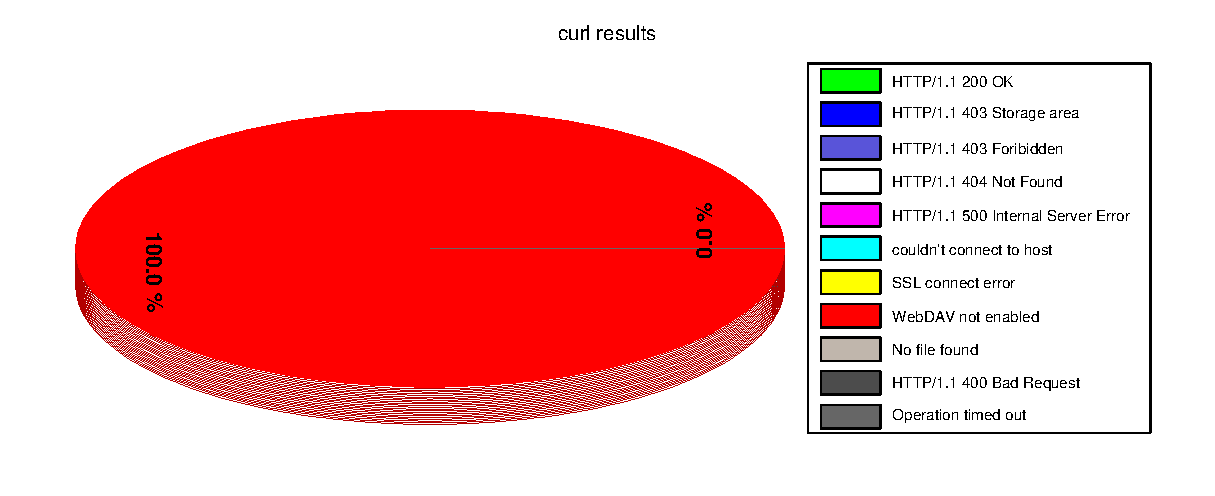
\includegraphics[width=\textwidth]{curlPiecanvas.eps}
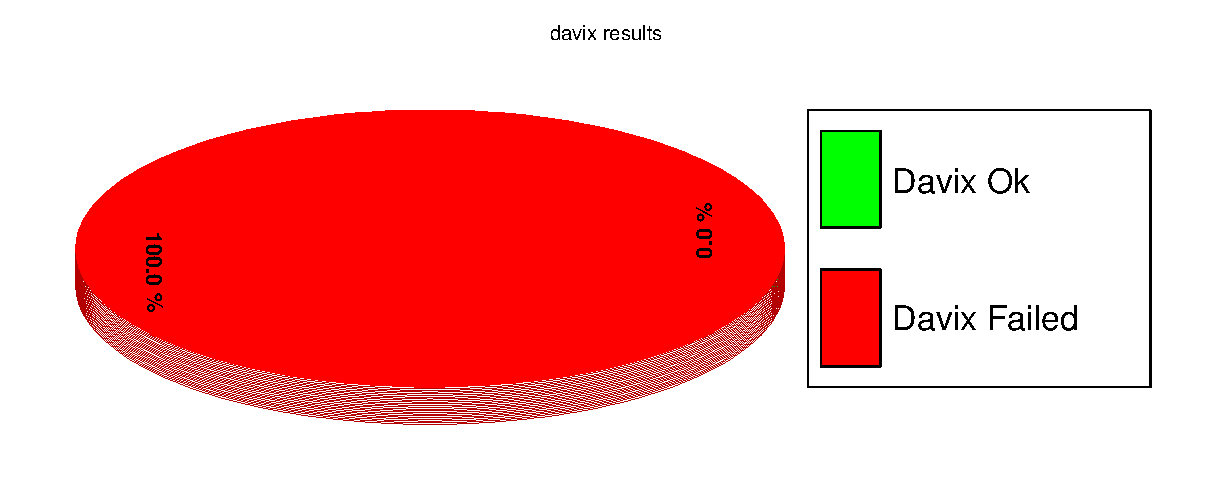
\includegraphics[width=\textwidth]{davixPiecanvas.eps}
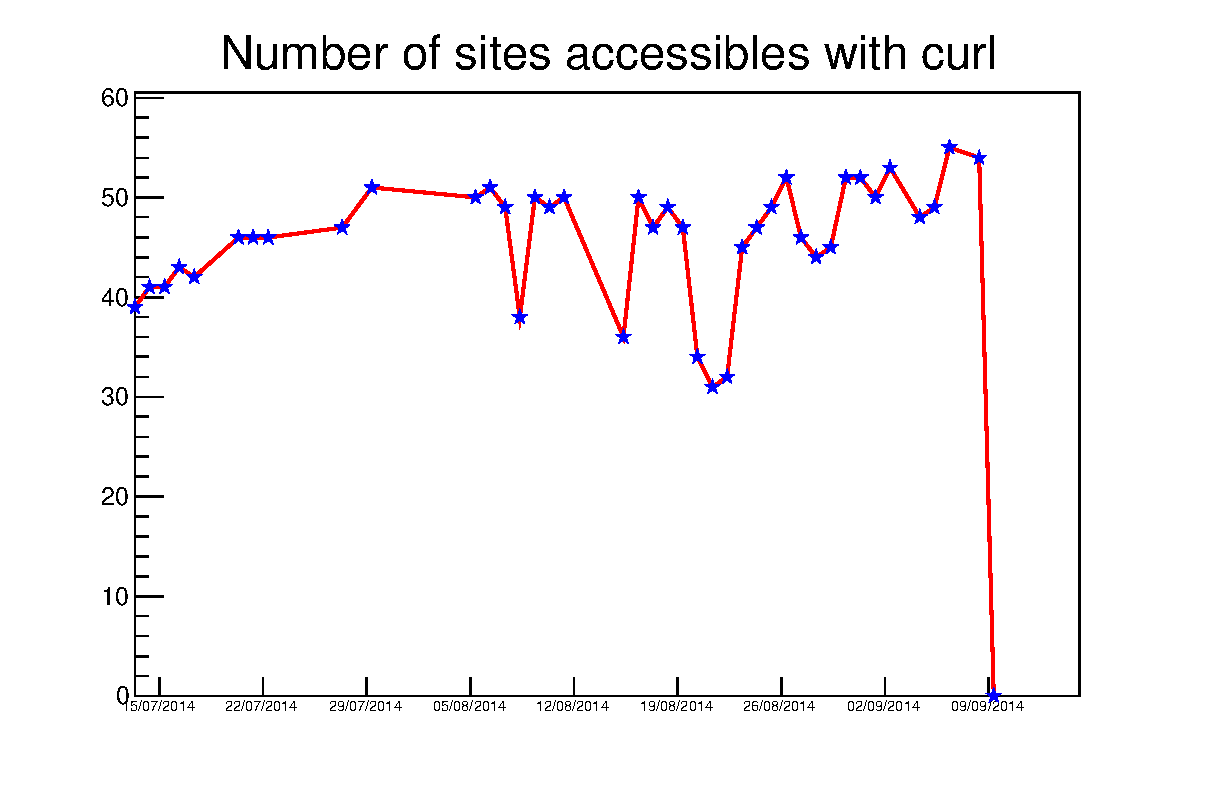
\includegraphics[width=\textwidth]{timeEvolutioncanvas.eps}


\subsection{CA}

\rule{\textwidth}{1pt}\\

\textcolor{red}{\normalsize{AUSTRALIA-ATLAS\_DATADISK}}\\

Storage: DPM, version: 1.8.8-1\\

File tested:\\
\footnotesize{https://rucio-lb-prod.cern.ch/redirect/mc12\_8TeV/NTUP\_COMMON.01344165.\_000057.root.1}\\

date: 10/09/14 at 11:19:44\\

curl output:  \textcolor{red}{New curl error that has to be identified}\\

davix result:  \textcolor{red}{Davix not tested}\\

\rule{\textwidth}{1pt}\\

\textcolor{red}{\normalsize{CA-MCGILL-CLUMEQ-T2\_DATADISK}}\\

Storage: StoRM, version: <FE:1.8.5><BE:1.11.4>\\

File tested:\\
\footnotesize{https://rucio-lb-prod.cern.ch/redirect/mc12\_8TeV/NTUP\_COMMON.01344384.\_000135.root.1}\\

date: 10/09/14 at 11:19:44\\

curl output:  \textcolor{red}{New curl error that has to be identified}\\

davix result:  \textcolor{red}{Davix not tested}\\

\rule{\textwidth}{1pt}\\

\textcolor{red}{\normalsize{CA-SCINET-T2\_DATADISK}}\\

Storage: dCache, version: 2.6.31\\

File tested:\\
\footnotesize{https://rucio-lb-prod.cern.ch/redirect/mc12\_8TeV/NTUP\_COMMON.01355386.\_000006.root.1}\\

date: 10/09/14 at 11:19:44\\

curl output:  \textcolor{red}{New curl error that has to be identified}\\

davix result:  \textcolor{red}{Davix not tested}\\

\rule{\textwidth}{1pt}\\

\textcolor{red}{\normalsize{TRIUMF-LCG2\_DATADISK}}\\

Storage: dCache, version: 2.6.30\\

File tested:\\
\footnotesize{https://rucio-lb-prod.cern.ch/redirect/mc12\_8TeV/NTUP\_COMMON.01317490.\_000001.root.1}\\

date: 10/09/14 at 11:19:44\\

curl output:  \textcolor{red}{New curl error that has to be identified}\\

davix result:  \textcolor{red}{Davix not tested}\\

\rule{\textwidth}{1pt}\\

\textcolor{red}{\normalsize{CA-VICTORIA-WESTGRID-T2\_DATADISK}}\\

Storage: dCache, version: 2.6.31\\

File tested:\\
\footnotesize{https://rucio-lb-prod.cern.ch/redirect/mc12\_8TeV/NTUP\_COMMON.01344434.\_000193.root.1}\\

date: 10/09/14 at 11:19:44\\

curl output:  \textcolor{red}{New curl error that has to be identified}\\

davix result:  \textcolor{red}{Davix not tested}\\

\rule{\textwidth}{1pt}\\

\textcolor{red}{\normalsize{SFU-LCG2\_DATADISK}}\\

Storage: dCache, version: 2.6.31\\

File tested:\\
\footnotesize{https://rucio-lb-prod.cern.ch/redirect/mc12\_8TeV/NTUP\_COMMON.01445382.\_002332.root.1}\\

date: 10/09/14 at 11:19:44\\

curl output:  \textcolor{red}{New curl error that has to be identified}\\

davix result:  \textcolor{red}{Davix not tested}\\

\subsection{DE}

\rule{\textwidth}{1pt}\\

\textcolor{red}{\normalsize{CSCS-LCG2\_DATADISK}}\\

Storage: dCache, version: 2.6.27\\

File tested:\\
\footnotesize{https://rucio-lb-prod.cern.ch/redirect/mc12\_8TeV/NTUP\_COMMON.01314827.\_000003.root.1}\\

date: 10/09/14 at 11:19:44\\

curl output:  \textcolor{red}{New curl error that has to be identified}\\

davix result:  \textcolor{red}{Davix not tested}\\

\rule{\textwidth}{1pt}\\

\textcolor{red}{\normalsize{CYFRONET-LCG2\_DATADISK}}\\

Storage: DPM, version: 1.8.8-1\\

File tested:\\
\footnotesize{https://rucio-lb-prod.cern.ch/redirect/mc12\_8TeV/NTUP\_COMMON.01378892.\_000066.root.1}\\

date: 10/09/14 at 11:19:45\\

curl output:  \textcolor{red}{New curl error that has to be identified}\\

davix result:  \textcolor{red}{Davix not tested}\\

\rule{\textwidth}{1pt}\\

\textcolor{red}{\normalsize{DESY-HH\_DATADISK}}\\

Storage: dCache, version: 2.8.3\\

File tested:\\
\footnotesize{https://rucio-lb-prod.cern.ch/redirect/mc12\_8TeV/NTUP\_COMMON.01383958.\_000068.root.1}\\

date: 10/09/14 at 11:19:45\\

curl output:  \textcolor{red}{New curl error that has to be identified}\\

davix result:  \textcolor{red}{Davix not tested}\\

\rule{\textwidth}{1pt}\\

\textcolor{red}{\normalsize{DESY-ZN\_DATADISK}}\\

Storage: dCache, version: 2.6.20\\

File tested:\\
\footnotesize{https://rucio-lb-prod.cern.ch/redirect/mc12\_8TeV/NTUP\_COMMON.01272994.\_000002.root.1}\\

date: 10/09/14 at 11:19:45\\

curl output:  \textcolor{red}{New curl error that has to be identified}\\

davix result:  \textcolor{red}{Davix not tested}\\

\rule{\textwidth}{1pt}\\

\textcolor{red}{\normalsize{FMPHI-UNIBA\_DATADISK}}\\

Storage: DPM, version: 1.8.8-1\\

File tested:\\
\footnotesize{https://rucio-lb-prod.cern.ch/redirect/mc12\_8TeV/NTUP\_COMMON.01344459.\_000006.root.1}\\

date: 10/09/14 at 11:19:45\\

curl output:  \textcolor{red}{New curl error that has to be identified}\\

davix result:  \textcolor{red}{Davix not tested}\\

\rule{\textwidth}{1pt}\\

\textcolor{red}{\normalsize{FZK-LCG2\_DATADISK}}\\

Storage: dCache, version: 2.6.28\\

File tested:\\
\footnotesize{https://rucio-lb-prod.cern.ch/redirect/mc12\_8TeV/NTUP\_COMMON.01368449.\_000034.root.1}\\

date: 10/09/14 at 11:19:45\\

curl output:  \textcolor{red}{New curl error that has to be identified}\\

davix result:  \textcolor{red}{Davix not tested}\\

\rule{\textwidth}{1pt}\\

\textcolor{red}{\normalsize{FZU-IPV6\_DATADISK}}\\

Storage: DPM, version: 1.8.7-3\\

File tested:\\
\footnotesize{https://rucio-lb-prod.cern.ch/redirect/mc12\_8TeV/NTUP\_COMMON.01368449.\_000034.root.1}\\

date: 10/09/14 at 11:19:45\\

curl output:  \textcolor{red}{WebDAV not enabled}\\

davix result:  \textcolor{red}{Davix not tested}\\

\rule{\textwidth}{1pt}\\

\textcolor{red}{\normalsize{GOEGRID\_DATADISK}}\\

Storage: dCache, version: 2.2.20\\

File tested:\\
\footnotesize{https://rucio-lb-prod.cern.ch/redirect/mc12\_8TeV/NTUP\_COMMON.01388892.\_000001.root.1}\\

date: 10/09/14 at 11:19:46\\

curl output:  \textcolor{red}{New curl error that has to be identified}\\

davix result:  \textcolor{red}{Davix not tested}\\

\rule{\textwidth}{1pt}\\

\textcolor{red}{\normalsize{HEPHY-UIBK\_DATADISK}}\\

Storage: DPM, version: 1.8.8-1\\

File tested:\\
\footnotesize{https://rucio-lb-prod.cern.ch/redirect/mc12\_8TeV/NTUP\_COMMON.01388892.\_000001.root.1}\\

date: 10/09/14 at 11:19:46\\

curl output:  \textcolor{red}{WebDAV not enabled}\\

davix result:  \textcolor{red}{Davix not tested}\\

\rule{\textwidth}{1pt}\\

\textcolor{red}{\normalsize{IEPSAS-KOSICE\_DATADISK}}\\

Storage: dCache, version: 2.6.30\\

File tested:\\
\footnotesize{https://rucio-lb-prod.cern.ch/redirect/mc12\_8TeV/NTUP\_COMMON.01353409.\_000001.root.1}\\

date: 10/09/14 at 11:19:46\\

curl output:  \textcolor{red}{New curl error that has to be identified}\\

davix result:  \textcolor{red}{Davix not tested}\\

\rule{\textwidth}{1pt}\\

\textcolor{red}{\normalsize{LRZ-LMU\_DATADISK}}\\

Storage: dCache, version: 2.6.31\\

File tested:\\
\footnotesize{https://rucio-lb-prod.cern.ch/redirect/mc12\_8TeV/NTUP\_COMMON.01311661.\_000239.root.1}\\

date: 10/09/14 at 11:19:46\\

curl output:  \textcolor{red}{New curl error that has to be identified}\\

davix result:  \textcolor{red}{Davix not tested}\\

\rule{\textwidth}{1pt}\\

\textcolor{red}{\normalsize{MPPMU\_DATADISK}}\\

Storage: dCache, version: 2.6.23\\

File tested:\\
\footnotesize{https://rucio-lb-prod.cern.ch/redirect/mc12\_8TeV/NTUP\_COMMON.01318243.\_000001.root.2}\\

date: 10/09/14 at 11:19:46\\

curl output:  \textcolor{red}{New curl error that has to be identified}\\

davix result:  \textcolor{red}{Davix not tested}\\

\rule{\textwidth}{1pt}\\

\textcolor{red}{\normalsize{PRAGUELCG2\_DATADISK}}\\

Storage: DPM, version: 1.8.7-3\\

File tested:\\
\footnotesize{https://rucio-lb-prod.cern.ch/redirect/mc12\_8TeV/NTUP\_COMMON.01318103.\_000002.root.1}\\

date: 10/09/14 at 11:19:46\\

curl output:  \textcolor{red}{New curl error that has to be identified}\\

davix result:  \textcolor{red}{Davix not tested}\\

\rule{\textwidth}{1pt}\\

\textcolor{red}{\normalsize{PSNC\_DATADISK}}\\

Storage: DPM, version: 1.8.8-1\\

File tested:\\
\footnotesize{https://rucio-lb-prod.cern.ch/redirect/mc12\_8TeV/NTUP\_COMMON.01312218.\_000002.root.2}\\

date: 10/09/14 at 11:19:47\\

curl output:  \textcolor{red}{New curl error that has to be identified}\\

davix result:  \textcolor{red}{Davix not tested}\\

\rule{\textwidth}{1pt}\\

\textcolor{red}{\normalsize{TUDRESDEN-ZIH\_DATADISK}}\\

Storage: dCache, version: 2.6.29\\

File tested:\\
\footnotesize{https://rucio-lb-prod.cern.ch/redirect/mc12\_8TeV/NTUP\_COMMON.01325732.\_000004.root.1}\\

date: 10/09/14 at 11:19:47\\

curl output:  \textcolor{red}{New curl error that has to be identified}\\

davix result:  \textcolor{red}{Davix not tested}\\

\rule{\textwidth}{1pt}\\

\textcolor{red}{\normalsize{UNI-FREIBURG\_DATADISK}}\\

Storage: dCache, version: 2.2.19\\

File tested:\\
\footnotesize{https://rucio-lb-prod.cern.ch/redirect/mc12\_8TeV/NTUP\_COMMON.01344660.\_000020.root.1}\\

date: 10/09/14 at 11:19:47\\

curl output:  \textcolor{red}{New curl error that has to be identified}\\

davix result:  \textcolor{red}{Davix not tested}\\

\rule{\textwidth}{1pt}\\

\textcolor{red}{\normalsize{UNI-SIEGEN-HEP\_DATADISK}}\\

Storage: DPM, version: 1.8.8-1\\

File tested:\\
\footnotesize{https://rucio-lb-prod.cern.ch/redirect/mc12\_8TeV/NTUP\_COMMON.01344660.\_000020.root.1}\\

date: 10/09/14 at 11:19:47\\

curl output:  \textcolor{red}{WebDAV not enabled}\\

davix result:  \textcolor{red}{Davix not tested}\\

\rule{\textwidth}{1pt}\\

\textcolor{red}{\normalsize{WUPPERTALPROD\_DATADISK}}\\

Storage: dCache, version: 2.6.30\\

File tested:\\
\footnotesize{https://rucio-lb-prod.cern.ch/redirect/mc12\_8TeV/NTUP\_COMMON.01344419.\_009610.root.1}\\

date: 10/09/14 at 11:19:47\\

curl output:  \textcolor{red}{New curl error that has to be identified}\\

davix result:  \textcolor{red}{Davix not tested}\\

\subsection{ES}

\rule{\textwidth}{1pt}\\

\textcolor{red}{\normalsize{PIC\_DATADISK}}\\

Storage: dCache, version: 2.6.29\\

File tested:\\
\footnotesize{https://rucio-lb-prod.cern.ch/redirect/mc12\_8TeV/NTUP\_COMMON.01452411.\_000012.root.3}\\

date: 10/09/14 at 11:19:47\\

curl output:  \textcolor{red}{New curl error that has to be identified}\\

davix result:  \textcolor{red}{Davix not tested}\\

\rule{\textwidth}{1pt}\\

\textcolor{red}{\normalsize{EELA-UTFSM\_DATADISK}}\\

Storage: dCache, version: 2.6.31\\

File tested:\\
\footnotesize{https://rucio-lb-prod.cern.ch/redirect/mc12\_8TeV/NTUP\_COMMON.01452394.\_000095.root.2}\\

date: 10/09/14 at 11:19:48\\

curl output:  \textcolor{red}{New curl error that has to be identified}\\

davix result:  \textcolor{red}{Davix not tested}\\

\rule{\textwidth}{1pt}\\

\textcolor{red}{\normalsize{IFAE\_DATADISK}}\\

Storage: dCache, version: 2.6.29\\

File tested:\\
\footnotesize{https://rucio-lb-prod.cern.ch/redirect/mc12\_8TeV/NTUP\_COMMON.01344293.\_000095.root.1}\\

date: 10/09/14 at 11:19:48\\

curl output:  \textcolor{red}{New curl error that has to be identified}\\

davix result:  \textcolor{red}{Davix not tested}\\

\rule{\textwidth}{1pt}\\

\textcolor{red}{\normalsize{IFIC-LCG2\_DATADISK}}\\

Storage: StoRM, version: <FE:1.8.4><BE:1.11.3>\\

File tested:\\
\footnotesize{https://rucio-lb-prod.cern.ch/redirect/mc12\_8TeV/NTUP\_COMMON.01389814.\_000013.root.1}\\

date: 10/09/14 at 11:19:48\\

curl output:  \textcolor{red}{New curl error that has to be identified}\\

davix result:  \textcolor{red}{Davix not tested}\\

\rule{\textwidth}{1pt}\\

\textcolor{red}{\normalsize{NCG-INGRID-PT\_DATADISK}}\\

Storage: StoRM, version: <FE:1.8.4><BE:1.11.3>\\

File tested:\\
\footnotesize{https://rucio-lb-prod.cern.ch/redirect/mc12\_8TeV/NTUP\_COMMON.01389814.\_000013.root.1}\\

date: 10/09/14 at 11:19:48\\

curl output:  \textcolor{red}{WebDAV not enabled}\\

davix result:  \textcolor{red}{Davix not tested}\\

\rule{\textwidth}{1pt}\\

\textcolor{red}{\normalsize{UAM-LCG2\_DATADISK}}\\

Storage: dCache, version: 2.6.31\\

File tested:\\
\footnotesize{https://rucio-lb-prod.cern.ch/redirect/mc12\_8TeV/NTUP\_COMMON.01390874.\_002183.root.1}\\

date: 10/09/14 at 11:19:48\\

curl output:  \textcolor{red}{New curl error that has to be identified}\\

davix result:  \textcolor{red}{Davix not tested}\\

\subsection{FR}

\rule{\textwidth}{1pt}\\

\textcolor{red}{\normalsize{IN2P3-CC\_DATADISK}}\\

Storage: dCache, version: 2.6.18\\

File tested:\\
\footnotesize{https://rucio-lb-prod.cern.ch/redirect/mc12\_8TeV/NTUP\_COMMON.01540501.\_006598.root.2}\\

date: 10/09/14 at 11:19:48\\

curl output:  \textcolor{red}{New curl error that has to be identified}\\

davix result:  \textcolor{red}{Davix not tested}\\

\rule{\textwidth}{1pt}\\

\textcolor{red}{\normalsize{BEIJING-LCG2\_DATADISK}}\\

Storage: DPM, version: 1.8.8-1\\

File tested:\\
\footnotesize{https://rucio-lb-prod.cern.ch/redirect/mc12\_8TeV/NTUP\_COMMON.01540501.\_006598.root.2}\\

date: 10/09/14 at 11:19:49\\

curl output:  \textcolor{red}{WebDAV not enabled}\\

davix result:  \textcolor{red}{Davix not tested}\\

\rule{\textwidth}{1pt}\\

\textcolor{red}{\normalsize{GRIF-IRFU\_DATADISK}}\\

Storage: DPM, version: 1.8.8-1\\

File tested:\\
\footnotesize{https://rucio-lb-prod.cern.ch/redirect/mc12\_8TeV/NTUP\_COMMON.01368425.\_000035.root.1}\\

date: 10/09/14 at 11:19:49\\

curl output:  \textcolor{red}{New curl error that has to be identified}\\

davix result:  \textcolor{red}{Davix not tested}\\

\rule{\textwidth}{1pt}\\

\textcolor{red}{\normalsize{GRIF-LAL\_DATADISK}}\\

Storage: DPM, version: 1.8.8-1\\

File tested:\\
\footnotesize{https://rucio-lb-prod.cern.ch/redirect/mc12\_8TeV/NTUP\_COMMON.01483261.\_000002.root.1}\\

date: 10/09/14 at 11:19:49\\

curl output:  \textcolor{red}{New curl error that has to be identified}\\

davix result:  \textcolor{red}{Davix not tested}\\

\rule{\textwidth}{1pt}\\

\textcolor{red}{\normalsize{GRIF-LPNHE\_DATADISK}}\\

Storage: DPM, version: 1.8.8-1\\

File tested:\\
\footnotesize{https://rucio-lb-prod.cern.ch/redirect/mc12\_8TeV/NTUP\_COMMON.01317911.\_000002.root.1}\\

date: 10/09/14 at 11:19:49\\

curl output:  \textcolor{red}{New curl error that has to be identified}\\

davix result:  \textcolor{red}{Davix not tested}\\

\rule{\textwidth}{1pt}\\

\textcolor{red}{\normalsize{IN2P3-CPPM\_DATADISK}}\\

Storage: DPM, version: 1.8.8-1\\

File tested:\\
\footnotesize{https://rucio-lb-prod.cern.ch/redirect/mc12\_8TeV/NTUP\_COMMON.01468113.\_000472.root.1}\\

date: 10/09/14 at 11:19:49\\

curl output:  \textcolor{red}{New curl error that has to be identified}\\

davix result:  \textcolor{red}{Davix not tested}\\

\rule{\textwidth}{1pt}\\

\textcolor{red}{\normalsize{IN2P3-LAPP\_DATADISK}}\\

Storage: DPM, version: 1.8.7-3\\

File tested:\\
\footnotesize{https://rucio-lb-prod.cern.ch/redirect/mc12\_8TeV/NTUP\_COMMON.01311510.\_000073.root.1}\\

date: 10/09/14 at 11:19:50\\

curl output:  \textcolor{red}{New curl error that has to be identified}\\

davix result:  \textcolor{red}{Davix not tested}\\

\rule{\textwidth}{1pt}\\

\textcolor{red}{\normalsize{IN2P3-LPC\_DATADISK}}\\

Storage: DPM, version: 1.8.8-1\\

File tested:\\
\footnotesize{https://rucio-lb-prod.cern.ch/redirect/mc12\_8TeV/NTUP\_COMMON.01313919.\_000174.root.1}\\

date: 10/09/14 at 11:19:50\\

curl output:  \textcolor{red}{New curl error that has to be identified}\\

davix result:  \textcolor{red}{Davix not tested}\\

\rule{\textwidth}{1pt}\\

\textcolor{red}{\normalsize{IN2P3-LPSC\_DATADISK}}\\

Storage: DPM, version: 1.8.7-3\\

File tested:\\
\footnotesize{https://rucio-lb-prod.cern.ch/redirect/mc12\_8TeV/NTUP\_COMMON.01398667.\_000006.root.1}\\

date: 10/09/14 at 11:19:50\\

curl output:  \textcolor{red}{New curl error that has to be identified}\\

davix result:  \textcolor{red}{Davix not tested}\\

\rule{\textwidth}{1pt}\\

\textcolor{red}{\normalsize{RO-02-NIPNE\_DATADISK}}\\

Storage: DPM, version: 1.8.8-1\\

File tested:\\
\footnotesize{https://rucio-lb-prod.cern.ch/redirect/mc12\_8TeV/NTUP\_COMMON.01452394.\_000008.root.1}\\

date: 10/09/14 at 11:19:50\\

curl output:  \textcolor{red}{New curl error that has to be identified}\\

davix result:  \textcolor{red}{Davix not tested}\\

\rule{\textwidth}{1pt}\\

\textcolor{red}{\normalsize{RO-14-ITIM\_DATADISK}}\\

Storage: DPM, version: 1.8.8-1\\

File tested:\\
\footnotesize{https://rucio-lb-prod.cern.ch/redirect/mc12\_8TeV/NTUP\_COMMON.01452394.\_000008.root.1}\\

date: 10/09/14 at 11:19:50\\

curl output:  \textcolor{red}{WebDAV not enabled}\\

davix result:  \textcolor{red}{Davix not tested}\\

\rule{\textwidth}{1pt}\\

\textcolor{red}{\normalsize{RO-07-NIPNE\_DATADISK}}\\

Storage: DPM, version: 1.8.8-1\\

File tested:\\
\footnotesize{https://rucio-lb-prod.cern.ch/redirect/mc12\_8TeV/NTUP\_COMMON.01315414.\_002498.root.2}\\

date: 10/09/14 at 11:19:50\\

curl output:  \textcolor{red}{New curl error that has to be identified}\\

davix result:  \textcolor{red}{Davix not tested}\\

\rule{\textwidth}{1pt}\\

\textcolor{red}{\normalsize{RO-16-UAIC\_DATADISK}}\\

Storage: DPM, version: 1.8.8-1\\

File tested:\\
\footnotesize{https://rucio-lb-prod.cern.ch/redirect/mc12\_8TeV/NTUP\_COMMON.01452394.\_000028.root.1}\\

date: 10/09/14 at 11:19:51\\

curl output:  \textcolor{red}{New curl error that has to be identified}\\

davix result:  \textcolor{red}{Davix not tested}\\

\rule{\textwidth}{1pt}\\

\textcolor{red}{\normalsize{TOKYO-LCG2\_DATADISK}}\\

Storage: DPM, version: 1.8.7-3\\

File tested:\\
\footnotesize{https://rucio-lb-prod.cern.ch/redirect/mc12\_8TeV/NTUP\_COMMON.01481216.\_009815.root.1}\\

date: 10/09/14 at 11:19:51\\

curl output:  \textcolor{red}{New curl error that has to be identified}\\

davix result:  \textcolor{red}{Davix not tested}\\

\subsection{IT}

\rule{\textwidth}{1pt}\\

\textcolor{red}{\normalsize{INFN-ROMA1\_DATADISK}}\\

Storage: DPM, version: 1.8.8-1\\

File tested:\\
\footnotesize{https://rucio-lb-prod.cern.ch/redirect/mc12\_8TeV/NTUP\_COMMON.01272994.\_000001.root.1}\\

date: 10/09/14 at 11:19:51\\

curl output:  \textcolor{red}{New curl error that has to be identified}\\

davix result:  \textcolor{red}{Davix not tested}\\

\rule{\textwidth}{1pt}\\

\textcolor{red}{\normalsize{INFN-NAPOLI-ATLAS\_DATADISK}}\\

Storage: DPM, version: 1.8.8-1\\

File tested:\\
\footnotesize{https://rucio-lb-prod.cern.ch/redirect/mc12\_8TeV/NTUP\_COMMON.01315325.\_000009.root.1}\\

date: 10/09/14 at 11:19:51\\

curl output:  \textcolor{red}{New curl error that has to be identified}\\

davix result:  \textcolor{red}{Davix not tested}\\

\rule{\textwidth}{1pt}\\

\textcolor{red}{\normalsize{INFN-FRASCATI\_DATADISK}}\\

Storage: DPM, version: 1.8.8-1\\

File tested:\\
\footnotesize{https://rucio-lb-prod.cern.ch/redirect/mc12\_8TeV/NTUP\_COMMON.01452646.\_000667.root.1}\\

date: 10/09/14 at 11:19:52\\

curl output:  \textcolor{red}{New curl error that has to be identified}\\

davix result:  \textcolor{red}{Davix not tested}\\

\rule{\textwidth}{1pt}\\

\textcolor{red}{\normalsize{INFN-MILANO-ATLASC\_DATADISK}}\\

Storage: StoRM, version: <FE:1.8.5><BE:1.11.3>\\

File tested:\\
\footnotesize{https://rucio-lb-prod.cern.ch/redirect/mc12\_8TeV/NTUP\_COMMON.01343871.\_000017.root.1}\\

date: 10/09/14 at 11:19:52\\

curl output:  \textcolor{red}{New curl error that has to be identified}\\

davix result:  \textcolor{red}{Davix not tested}\\

\subsection{ND}

\rule{\textwidth}{1pt}\\

\textcolor{red}{\normalsize{NDGF-T1\_DATADISK}}\\

Storage: dCache, version: 2.10.3\\

File tested:\\
\footnotesize{https://rucio-lb-prod.cern.ch/redirect/mc12\_8TeV/NTUP\_COMMON.01281679.\_000011.root.1}\\

date: 10/09/14 at 11:19:52\\

curl output:  \textcolor{red}{New curl error that has to be identified}\\

davix result:  \textcolor{red}{Davix not tested}\\

\rule{\textwidth}{1pt}\\

\textcolor{red}{\normalsize{SE-SNIC-T2\_DATADISK}}\\

Storage: dCache, version: 2.7.16\\

File tested:\\
\footnotesize{https://rucio-lb-prod.cern.ch/redirect/mc12\_8TeV/NTUP\_COMMON.01452394.\_000171.root.1}\\

date: 10/09/14 at 11:19:52\\

curl output:  \textcolor{red}{New curl error that has to be identified}\\

davix result:  \textcolor{red}{Davix not tested}\\

\rule{\textwidth}{1pt}\\

\textcolor{red}{\normalsize{UNIBE-LHEP\_DATADISK}}\\

Storage: DPM, version: 1.8.8-1\\

File tested:\\
\footnotesize{https://rucio-lb-prod.cern.ch/redirect/mc12\_8TeV/NTUP\_COMMON.01452394.\_000037.root.1}\\

date: 10/09/14 at 11:19:52\\

curl output:  \textcolor{red}{New curl error that has to be identified}\\

davix result:  \textcolor{red}{Davix not tested}\\

\rule{\textwidth}{1pt}\\

\textcolor{red}{\normalsize{CERN-PROD\_DATADISK}}\\

Storage: unknown, version: unknown\\

File tested:\\
\footnotesize{https://rucio-lb-prod.cern.ch/redirect/mc12\_8TeV/NTUP\_COMMON.01349021.\_000006.root.1}\\

date: 10/09/14 at 11:19:52\\

curl output:  \textcolor{red}{New curl error that has to be identified}\\

davix result:  \textcolor{red}{Davix not tested}\\

\subsection{NL}

\rule{\textwidth}{1pt}\\

\textcolor{red}{\normalsize{IL-TAU-HEP\_DATADISK}}\\

Storage: StoRM, version: <FE:1.8.3-1><BE:1.11.2>\\

File tested:\\
\footnotesize{https://rucio-lb-prod.cern.ch/redirect/mc12\_8TeV/NTUP\_COMMON.01349021.\_000006.root.1}\\

date: 10/09/14 at 11:19:53\\

curl output:  \textcolor{red}{WebDAV not enabled}\\

davix result:  \textcolor{red}{Davix not tested}\\

\rule{\textwidth}{1pt}\\

\textcolor{red}{\normalsize{ITEP\_DATADISK}}\\

Storage: dCache, version: 2.6.17\\

File tested:\\
\footnotesize{https://rucio-lb-prod.cern.ch/redirect/mc12\_8TeV/NTUP\_COMMON.01349021.\_000006.root.1}\\

date: 10/09/14 at 11:19:53\\

curl output:  \textcolor{red}{WebDAV not enabled}\\

davix result:  \textcolor{red}{Davix not tested}\\

\rule{\textwidth}{1pt}\\

\textcolor{red}{\normalsize{JINR-LCG2\_DATADISK}}\\

Storage: dCache, version: 2.6.31\\

File tested:\\
\footnotesize{https://rucio-lb-prod.cern.ch/redirect/mc12\_8TeV/NTUP\_COMMON.01452394.\_000008.root.1}\\

date: 10/09/14 at 11:19:53\\

curl output:  \textcolor{red}{New curl error that has to be identified}\\

davix result:  \textcolor{red}{Davix not tested}\\

\rule{\textwidth}{1pt}\\

\textcolor{red}{\normalsize{NIKHEF-ELPROD\_DATADISK}}\\

Storage: DPM, version: 1.8.8-1\\

File tested:\\
\footnotesize{https://rucio-lb-prod.cern.ch/redirect/mc12\_8TeV/NTUP\_COMMON.01325732.\_000001.root.1}\\

date: 10/09/14 at 11:19:53\\

curl output:  \textcolor{red}{New curl error that has to be identified}\\

davix result:  \textcolor{red}{Davix not tested}\\

\rule{\textwidth}{1pt}\\

\textcolor{red}{\normalsize{RRC-KI\_DATADISK}}\\

Storage: DPM, version: 1.8.8-1\\

File tested:\\
\footnotesize{https://rucio-lb-prod.cern.ch/redirect/mc12\_8TeV/NTUP\_COMMON.01325732.\_000001.root.1}\\

date: 10/09/14 at 11:19:53\\

curl output:  \textcolor{red}{WebDAV not enabled}\\

davix result:  \textcolor{red}{Davix not tested}\\

\rule{\textwidth}{1pt}\\

\textcolor{red}{\normalsize{RU-MOSCOW-FIAN-LCG2\_DATADISK}}\\

Storage: DPM, version: 1.8.7-3\\

File tested:\\
\footnotesize{https://rucio-lb-prod.cern.ch/redirect/mc12\_8TeV/NTUP\_COMMON.01325732.\_000001.root.1}\\

date: 10/09/14 at 11:19:53\\

curl output:  \textcolor{red}{WebDAV not enabled}\\

davix result:  \textcolor{red}{Davix not tested}\\

\rule{\textwidth}{1pt}\\

\textcolor{red}{\normalsize{RU-PNPI\_DATADISK}}\\

Storage: DPM, version: 1.8.8-1\\

File tested:\\
\footnotesize{https://rucio-lb-prod.cern.ch/redirect/mc12\_8TeV/NTUP\_COMMON.01325732.\_000001.root.1}\\

date: 10/09/14 at 11:19:53\\

curl output:  \textcolor{red}{WebDAV not enabled}\\

davix result:  \textcolor{red}{Davix not tested}\\

\rule{\textwidth}{1pt}\\

\textcolor{red}{\normalsize{RU-PROTVINO-IHEP\_DATADISK}}\\

Storage: dCache, version: 2.6.17\\

File tested:\\
\footnotesize{https://rucio-lb-prod.cern.ch/redirect/mc12\_8TeV/NTUP\_COMMON.01445365.\_000389.root.1}\\

date: 10/09/14 at 11:19:53\\

curl output:  \textcolor{red}{New curl error that has to be identified}\\

davix result:  \textcolor{red}{Davix not tested}\\

\rule{\textwidth}{1pt}\\

\textcolor{red}{\normalsize{SARA-MATRIX\_DATADISK}}\\

Storage: dCache, version: 2.6.32\\

File tested:\\
\footnotesize{https://rucio-lb-prod.cern.ch/redirect/mc12\_8TeV/NTUP\_COMMON.01344441.\_000096.root.1}\\

date: 10/09/14 at 11:19:54\\

curl output:  \textcolor{red}{New curl error that has to be identified}\\

davix result:  \textcolor{red}{Davix not tested}\\

\rule{\textwidth}{1pt}\\

\textcolor{red}{\normalsize{TECHNION-HEP\_DATADISK}}\\

Storage: StoRM, version: <FE:1.8.5><BE:1.11.4>\\

File tested:\\
\footnotesize{https://rucio-lb-prod.cern.ch/redirect/mc12\_8TeV/NTUP\_COMMON.01344441.\_000096.root.1}\\

date: 10/09/14 at 11:19:54\\

curl output:  \textcolor{red}{WebDAV not enabled}\\

davix result:  \textcolor{red}{Davix not tested}\\

\rule{\textwidth}{1pt}\\

\textcolor{red}{\normalsize{TR-10-ULAKBIM\_DATADISK}}\\

Storage: DPM, version: 1.8.7-3\\

File tested:\\
\footnotesize{https://rucio-lb-prod.cern.ch/redirect/mc12\_8TeV/NTUP\_COMMON.01452394.\_000183.root.2}\\

date: 10/09/14 at 11:19:54\\

curl output:  \textcolor{red}{New curl error that has to be identified}\\

davix result:  \textcolor{red}{Davix not tested}\\

\rule{\textwidth}{1pt}\\

\textcolor{red}{\normalsize{WEIZMANN-LCG2\_DATADISK}}\\

Storage: StoRM, version: <FE:1.8.5><BE:1.11.4>\\

File tested:\\
\footnotesize{https://rucio-lb-prod.cern.ch/redirect/mc12\_8TeV/NTUP\_COMMON.01452394.\_000183.root.2}\\

date: 10/09/14 at 11:19:54\\

curl output:  \textcolor{red}{WebDAV not enabled}\\

davix result:  \textcolor{red}{Davix not tested}\\

\subsection{UK}

\rule{\textwidth}{1pt}\\

\textcolor{red}{\normalsize{RAL-LCG2\_DATADISK}}\\

Storage: CASTOR, version: 2.1.14-13\\

File tested:\\
\footnotesize{https://rucio-lb-prod.cern.ch/redirect/mc12\_8TeV/NTUP\_COMMON.01452394.\_000183.root.2}\\

date: 10/09/14 at 11:19:54\\

curl output:  \textcolor{red}{WebDAV not enabled}\\

davix result:  \textcolor{red}{Davix not tested}\\

\rule{\textwidth}{1pt}\\

\textcolor{red}{\normalsize{UKI-LT2-BRUNEL\_DATADISK}}\\

Storage: DPM, version: 1.8.8-1\\

File tested:\\
\footnotesize{https://rucio-lb-prod.cern.ch/redirect/mc12\_8TeV/NTUP\_COMMON.01452394.\_000152.root.1}\\

date: 10/09/14 at 11:19:55\\

curl output:  \textcolor{red}{New curl error that has to be identified}\\

davix result:  \textcolor{red}{Davix not tested}\\

\rule{\textwidth}{1pt}\\

\textcolor{red}{\normalsize{UKI-LT2-IC-HEP\_DATADISK}}\\

Storage: dCache, version: 2.6.20\\

File tested:\\
\footnotesize{https://rucio-lb-prod.cern.ch/redirect/mc12\_8TeV/NTUP\_COMMON.01452394.\_000148.root.1}\\

date: 10/09/14 at 11:19:55\\

curl output:  \textcolor{red}{New curl error that has to be identified}\\

davix result:  \textcolor{red}{Davix not tested}\\

\rule{\textwidth}{1pt}\\

\textcolor{red}{\normalsize{UKI-LT2-QMUL\_DATADISK}}\\

Storage: StoRM, version: <FE:1.8.5><BE:1.11.4>\\

File tested:\\
\footnotesize{https://rucio-lb-prod.cern.ch/redirect/mc12\_8TeV/NTUP\_COMMON.01483457.\_000002.root.1}\\

date: 10/09/14 at 11:19:55\\

curl output:  \textcolor{red}{New curl error that has to be identified}\\

davix result:  \textcolor{red}{Davix not tested}\\

\rule{\textwidth}{1pt}\\

\textcolor{red}{\normalsize{UKI-LT2-RHUL\_DATADISK}}\\

Storage: DPM, version: 1.8.8-1\\

File tested:\\
\footnotesize{https://rucio-lb-prod.cern.ch/redirect/mc12\_8TeV/NTUP\_COMMON.01313961.\_000081.root.1}\\

date: 10/09/14 at 11:19:55\\

curl output:  \textcolor{red}{New curl error that has to be identified}\\

davix result:  \textcolor{red}{Davix not tested}\\

\rule{\textwidth}{1pt}\\

\textcolor{red}{\normalsize{UKI-LT2-UCL-HEP\_DATADISK}}\\

Storage: DPM, version: 1.8.8-1\\

File tested:\\
\footnotesize{https://rucio-lb-prod.cern.ch/redirect/mc12\_8TeV/NTUP\_COMMON.01315387.\_000074.root.1}\\

date: 10/09/14 at 11:19:55\\

curl output:  \textcolor{red}{New curl error that has to be identified}\\

davix result:  \textcolor{red}{Davix not tested}\\

\rule{\textwidth}{1pt}\\

\textcolor{red}{\normalsize{UKI-NORTHGRID-LANCS-HEP\_DATADISK}}\\

Storage: DPM, version: 1.8.8-1\\

File tested:\\
\footnotesize{https://rucio-lb-prod.cern.ch/redirect/mc12\_8TeV/NTUP\_HSG2.01447850.\_000004.root.1}\\

date: 10/09/14 at 11:19:56\\

curl output:  \textcolor{red}{New curl error that has to be identified}\\

davix result:  \textcolor{red}{Davix not tested}\\

\rule{\textwidth}{1pt}\\

\textcolor{red}{\normalsize{UKI-NORTHGRID-LIV-HEP\_DATADISK}}\\

Storage: DPM, version: 1.8.8-1\\

File tested:\\
\footnotesize{https://rucio-lb-prod.cern.ch/redirect/mc12\_8TeV/NTUP\_COMMON.01388867.\_000002.root.1}\\

date: 10/09/14 at 11:19:56\\

curl output:  \textcolor{red}{New curl error that has to be identified}\\

davix result:  \textcolor{red}{Davix not tested}\\

\rule{\textwidth}{1pt}\\

\textcolor{red}{\normalsize{UKI-NORTHGRID-MAN-HEP\_DATADISK}}\\

Storage: DPM, version: 1.8.7-3\\

File tested:\\
\footnotesize{https://rucio-lb-prod.cern.ch/redirect/mc12\_8TeV/NTUP\_COMMON.01426577.\_001524.root.1}\\

date: 10/09/14 at 11:19:56\\

curl output:  \textcolor{red}{New curl error that has to be identified}\\

davix result:  \textcolor{red}{Davix not tested}\\

\rule{\textwidth}{1pt}\\

\textcolor{red}{\normalsize{UKI-NORTHGRID-SHEF-HEP\_DATADISK}}\\

Storage: DPM, version: 1.8.7-3\\

File tested:\\
\footnotesize{https://rucio-lb-prod.cern.ch/redirect/mc12\_8TeV/NTUP\_COMMON.01483261.\_000371.root.1}\\

date: 10/09/14 at 11:19:56\\

curl output:  \textcolor{red}{New curl error that has to be identified}\\

davix result:  \textcolor{red}{Davix not tested}\\

\rule{\textwidth}{1pt}\\

\textcolor{red}{\normalsize{UKI-SCOTGRID-DURHAM\_DATADISK}}\\

Storage: DPM, version: 1.8.8-1\\

File tested:\\
\footnotesize{https://rucio-lb-prod.cern.ch/redirect/mc12\_8TeV/NTUP\_COMMON.01483261.\_000371.root.1}\\

date: 10/09/14 at 11:19:56\\

curl output:  \textcolor{red}{WebDAV not enabled}\\

davix result:  \textcolor{red}{Davix not tested}\\

\rule{\textwidth}{1pt}\\

\textcolor{red}{\normalsize{UKI-SCOTGRID-ECDF\_DATADISK}}\\

Storage: DPM, version: 1.8.8-1\\

File tested:\\
\footnotesize{https://rucio-lb-prod.cern.ch/redirect/mc12\_8TeV/NTUP\_COMMON.01311762.\_000071.root.2}\\

date: 10/09/14 at 11:19:57\\

curl output:  \textcolor{red}{New curl error that has to be identified}\\

davix result:  \textcolor{red}{Davix not tested}\\

\rule{\textwidth}{1pt}\\

\textcolor{red}{\normalsize{UKI-SCOTGRID-GLASGOW\_DATADISK}}\\

Storage: DPM, version: 1.8.8-1\\

File tested:\\
\footnotesize{https://rucio-lb-prod.cern.ch/redirect/mc12\_8TeV/NTUP\_COMMON.01313980.\_000021.root.1}\\

date: 10/09/14 at 11:19:57\\

curl output:  \textcolor{red}{New curl error that has to be identified}\\

davix result:  \textcolor{red}{Davix not tested}\\

\rule{\textwidth}{1pt}\\

\textcolor{red}{\normalsize{UKI-SOUTHGRID-BHAM-HEP\_DATADISK}}\\

Storage: DPM, version: 1.8.8-1\\

File tested:\\
\footnotesize{https://rucio-lb-prod.cern.ch/redirect/mc12\_8TeV/NTUP\_COMMON.01311711.\_000008.root.1}\\

date: 10/09/14 at 11:19:57\\

curl output:  \textcolor{red}{New curl error that has to be identified}\\

davix result:  \textcolor{red}{Davix not tested}\\

\rule{\textwidth}{1pt}\\

\textcolor{red}{\normalsize{UKI-SOUTHGRID-CAM-HEP\_DATADISK}}\\

Storage: DPM, version: 1.8.8-1\\

File tested:\\
\footnotesize{https://rucio-lb-prod.cern.ch/redirect/mc12\_8TeV/NTUP\_COMMON.01344032.\_000118.root.1}\\

date: 10/09/14 at 11:19:57\\

curl output:  \textcolor{red}{New curl error that has to be identified}\\

davix result:  \textcolor{red}{Davix not tested}\\

\rule{\textwidth}{1pt}\\

\textcolor{red}{\normalsize{UKI-SOUTHGRID-OX-HEP\_DATADISK}}\\

Storage: DPM, version: 1.8.8-1\\

File tested:\\
\footnotesize{https://rucio-lb-prod.cern.ch/redirect/mc12\_8TeV/NTUP\_COMMON.01360831.\_000001.root.1}\\

date: 10/09/14 at 11:19:57\\

curl output:  \textcolor{red}{New curl error that has to be identified}\\

davix result:  \textcolor{red}{Davix not tested}\\

\rule{\textwidth}{1pt}\\

\textcolor{red}{\normalsize{UKI-SOUTHGRID-RALPP\_DATADISK}}\\

Storage: dCache, version: 2.6.23\\

File tested:\\
\footnotesize{https://rucio-lb-prod.cern.ch/redirect/mc12\_8TeV/NTUP\_COMMON.01273005.\_000715.root.10}\\

date: 10/09/14 at 11:19:58\\

curl output:  \textcolor{red}{New curl error that has to be identified}\\

davix result:  \textcolor{red}{Davix not tested}\\

\rule{\textwidth}{1pt}\\

\textcolor{red}{\normalsize{UKI-SOUTHGRID-SUSX\_DATADISK}}\\

Storage: StoRM, version: <FE:1.8.5><BE:1.11.4>\\

File tested:\\
\footnotesize{https://rucio-lb-prod.cern.ch/redirect/mc12\_8TeV/NTUP\_COMMON.01273005.\_000715.root.10}\\

date: 10/09/14 at 11:19:58\\

curl output:  \textcolor{red}{WebDAV not enabled}\\

davix result:  \textcolor{red}{Davix not tested}\\

\subsection{US}

\rule{\textwidth}{1pt}\\

\textcolor{red}{\normalsize{AGLT2\_DATADISK}}\\

Storage: dCache, version: 2.6.31\\

File tested:\\
\footnotesize{https://rucio-lb-prod.cern.ch/redirect/mc12\_8TeV/NTUP\_COMMON.01398752.\_000072.root.1}\\

date: 10/09/14 at 11:19:58\\

curl output:  \textcolor{red}{New curl error that has to be identified}\\

davix result:  \textcolor{red}{Davix not tested}\\

\rule{\textwidth}{1pt}\\

\textcolor{red}{\normalsize{ANLASC\_DATADISK}}\\

Storage: unknown, version: unknown\\

File tested:\\
\footnotesize{https://rucio-lb-prod.cern.ch/redirect/mc12\_8TeV/NTUP\_COMMON.01398752.\_000072.root.1}\\

date: 10/09/14 at 11:19:58\\

curl output:  \textcolor{red}{WebDAV not enabled}\\

davix result:  \textcolor{red}{Davix not tested}\\

\rule{\textwidth}{1pt}\\

\textcolor{red}{\normalsize{BNL-OSG2\_DATADISK}}\\

Storage: dCache, version: 2.6.18\\

File tested:\\
\footnotesize{https://rucio-lb-prod.cern.ch/redirect/mc12\_8TeV/NTUP\_COMMON.01540573.\_000572.root.1}\\

date: 10/09/14 at 11:19:58\\

curl output:  \textcolor{red}{New curl error that has to be identified}\\

davix result:  \textcolor{red}{Davix not tested}\\

\rule{\textwidth}{1pt}\\

\textcolor{red}{\normalsize{LUCILLE\_DATADISK}}\\

Storage: unknown, version: unknown\\

File tested:\\
\footnotesize{https://rucio-lb-prod.cern.ch/redirect/mc12\_8TeV/NTUP\_COMMON.01540573.\_000572.root.1}\\

date: 10/09/14 at 11:19:59\\

curl output:  \textcolor{red}{WebDAV not enabled}\\

davix result:  \textcolor{red}{Davix not tested}\\

\rule{\textwidth}{1pt}\\

\textcolor{red}{\normalsize{MWT2\_DATADISK}}\\

Storage: dCache, version: 2.6.30\\

File tested:\\
\footnotesize{https://rucio-lb-prod.cern.ch/redirect/mc12\_8TeV/NTUP\_COMMON.01344361.\_005613.root.1}\\

date: 10/09/14 at 11:19:59\\

curl output:  \textcolor{red}{New curl error that has to be identified}\\

davix result:  \textcolor{red}{Davix not tested}\\

\rule{\textwidth}{1pt}\\

\textcolor{red}{\normalsize{NET2\_DATADISK}}\\

Storage: unknown, version: unknown\\

File tested:\\
\footnotesize{https://rucio-lb-prod.cern.ch/redirect/mc12\_8TeV/NTUP\_COMMON.01344361.\_005613.root.1}\\

date: 10/09/14 at 11:19:59\\

curl output:  \textcolor{red}{WebDAV not enabled}\\

davix result:  \textcolor{red}{Davix not tested}\\

\rule{\textwidth}{1pt}\\

\textcolor{red}{\normalsize{OUHEP\_OSG\_DATADISK}}\\

Storage: unknown, version: unknown\\

File tested:\\
\footnotesize{https://rucio-lb-prod.cern.ch/redirect/mc12\_8TeV/NTUP\_COMMON.01344361.\_005613.root.1}\\

date: 10/09/14 at 11:19:59\\

curl output:  \textcolor{red}{WebDAV not enabled}\\

davix result:  \textcolor{red}{Davix not tested}\\

\rule{\textwidth}{1pt}\\

\textcolor{red}{\normalsize{OU\_OCHEP\_SWT2\_DATADISK}}\\

Storage: unknown, version: unknown\\

File tested:\\
\footnotesize{https://rucio-lb-prod.cern.ch/redirect/mc12\_8TeV/NTUP\_COMMON.01344361.\_005613.root.1}\\

date: 10/09/14 at 11:19:59\\

curl output:  \textcolor{red}{WebDAV not enabled}\\

davix result:  \textcolor{red}{Davix not tested}\\

\rule{\textwidth}{1pt}\\

\textcolor{red}{\normalsize{SLACXRD\_DATADISK}}\\

Storage: unknown, version: unknown\\

File tested:\\
\footnotesize{https://rucio-lb-prod.cern.ch/redirect/mc12\_8TeV/NTUP\_COMMON.01344361.\_005613.root.1}\\

date: 10/09/14 at 11:19:59\\

curl output:  \textcolor{red}{WebDAV not enabled}\\

davix result:  \textcolor{red}{Davix not tested}\\

\rule{\textwidth}{1pt}\\

\textcolor{red}{\normalsize{SWT2\_CPB\_DATADISK}}\\

Storage: unknown, version: unknown\\

File tested:\\
\footnotesize{https://rucio-lb-prod.cern.ch/redirect/mc12\_8TeV/NTUP\_COMMON.01344361.\_005613.root.1}\\

date: 10/09/14 at 11:19:59\\

curl output:  \textcolor{red}{WebDAV not enabled}\\

davix result:  \textcolor{red}{Davix not tested}\\

\rule{\textwidth}{1pt}\\

\textcolor{red}{\normalsize{UTA\_SWT2\_DATADISK}}\\

Storage: unknown, version: unknown\\

File tested:\\
\footnotesize{https://rucio-lb-prod.cern.ch/redirect/mc12\_8TeV/NTUP\_COMMON.01344361.\_005613.root.1}\\

date: 10/09/14 at 11:19:59\\

curl output:  \textcolor{red}{WebDAV not enabled}\\

davix result:  \textcolor{red}{Davix not tested}\\

\rule{\textwidth}{1pt}\\

\textcolor{red}{\normalsize{TAIWAN-LCG2\_DATADISK}}\\

Storage: DPM, version: 1.8.8-1\\

File tested:\\
\footnotesize{https://rucio-lb-prod.cern.ch/redirect/mc12\_8TeV/NTUP\_COMMON.01318884.\_000001.root.1}\\

date: 10/09/14 at 11:20:00\\

curl output:  \textcolor{red}{New curl error that has to be identified}\\

davix result:  \textcolor{red}{Davix not tested}\\


%The objective of this test is to check how many file are successfully opened and read for each SE of the grid.\\

A job is sent to each principal queues of the grid. This jobs repeats 100 times the following steps:
\begin{itemize}
	\item A list of file is generated on the same way than for the first test but this time only for sites that belongs to the cloud where is running the job.
	\item A compiled C++/root program opens the file read all events of the branches \textit{el\_n} and \textit{mu\_n} of tree \textit{physics} and measure the time to complete the reading part.
	\item Am histogram is filled with the event's rate of the recent read file
\end{itemize}

In this test we are not interested in the performances of Davix, we just want to know if it's working. The matrix presented in this part are done by cloud (the taiwanees cloud contains only one site to enable remote access it's tested with the US cloud). The X-axe corresponds to the queue where ran the job, the Y-axe corresponds to the Datadisk that contains the file we are trying to access. The number in the box corresponds the rate of file successfully read. When the box is empty is just mean that they all failed.
\vspace{1ex}

%\vspace{1ex}\\

\vspace{1ex}\\

\vspace{1ex}\\

\vspace{1ex}\\

\vspace{1ex}\\

\vspace{1ex}\\

\vspace{1ex}\\

\vspace{1ex}\\

\vspace{1ex}\\


\section{The WebDAV events rate}

The objective of this test is to check how many file are successfully opened and read for each SE of the grid.\\

A job is sent to each principal queues of the grid. This jobs repeats 100 times the following steps:
\begin{itemize}
        \item A list of file is generated on the same way than for the first test but this time only for sites that belongs to the cloud where is running the job.
        \item A compiled C++/root program opens the file read all events of the branches \textit{el\_n} and \textit{mu\_n} of tree \textit{physics} and measure the time to complete the reading part.
        \item Am histogram is filled with the event's rate of the recent read file
\end{itemize}

In this test we are not interested in the performances of Davix, we just want to know if it's working. The matrix presented in this part are done by cloud (the taiwanees cloud contains only one site to enable remote access it's tested with the US cloud). The X-axe corresponds to the queue where ran the job, the Y-axe corresponds to the Datadisk that contains the file we are trying to access. The number in the box corresponds the rate of file successfully read. When the box is empty is just mean that they all failed. 
\vspace{1ex}

\vspace{1ex}

\subsection{Cloud CA}
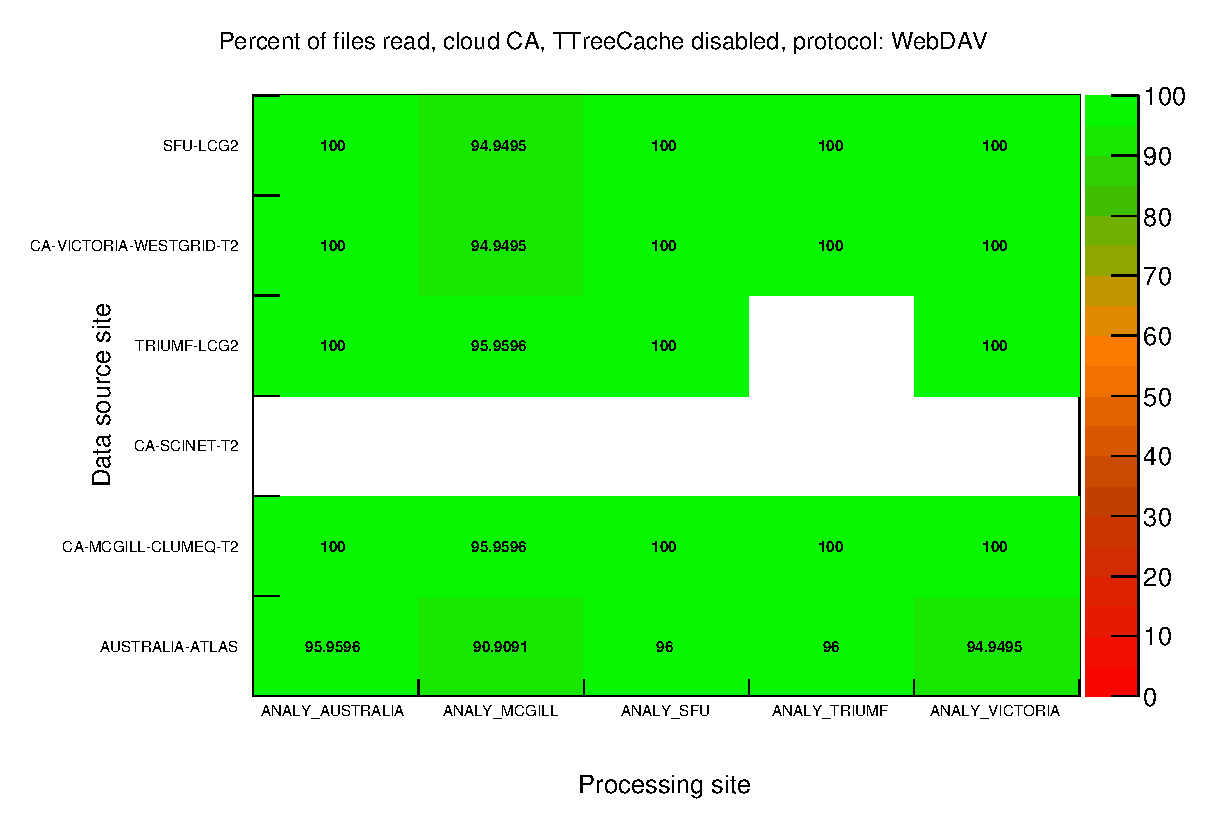
\includegraphics[width=\textwidth]{CA_PerCentFile.eps}
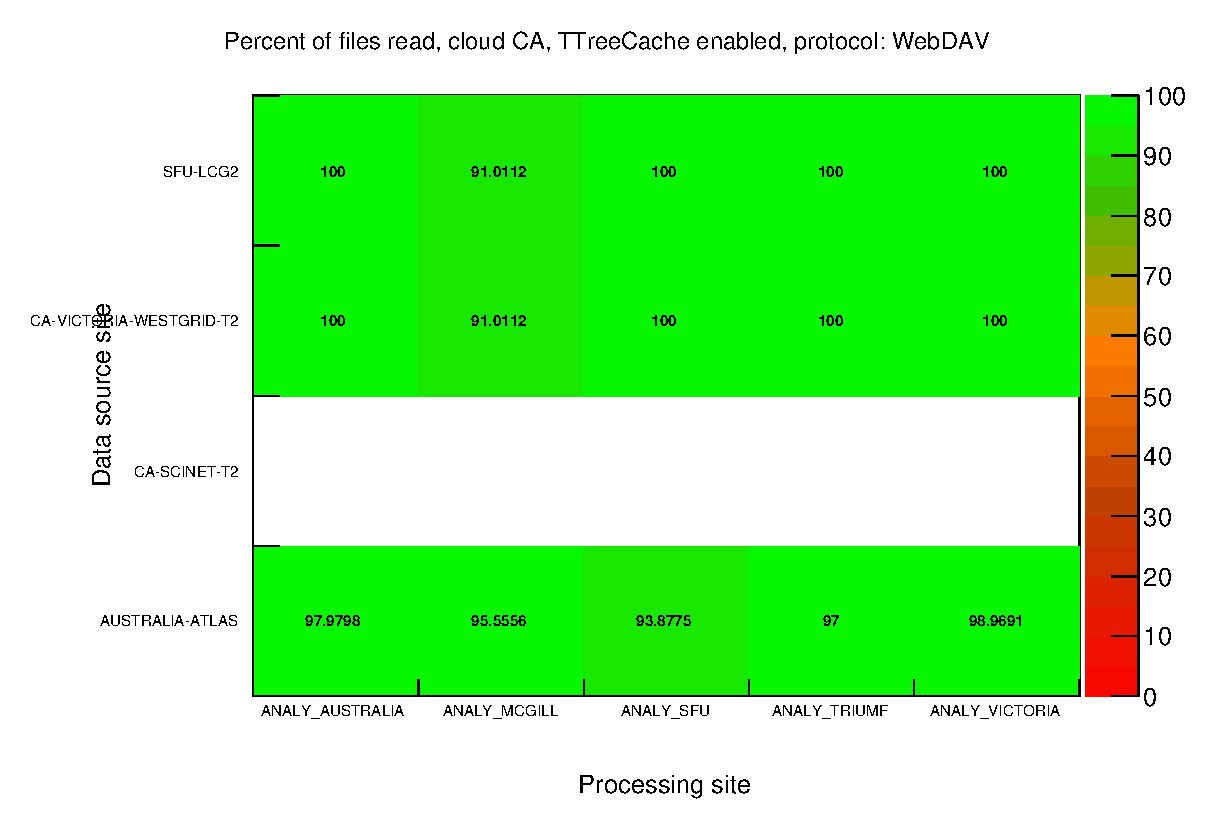
\includegraphics[width=\textwidth]{CA_tPerCentFile.eps}
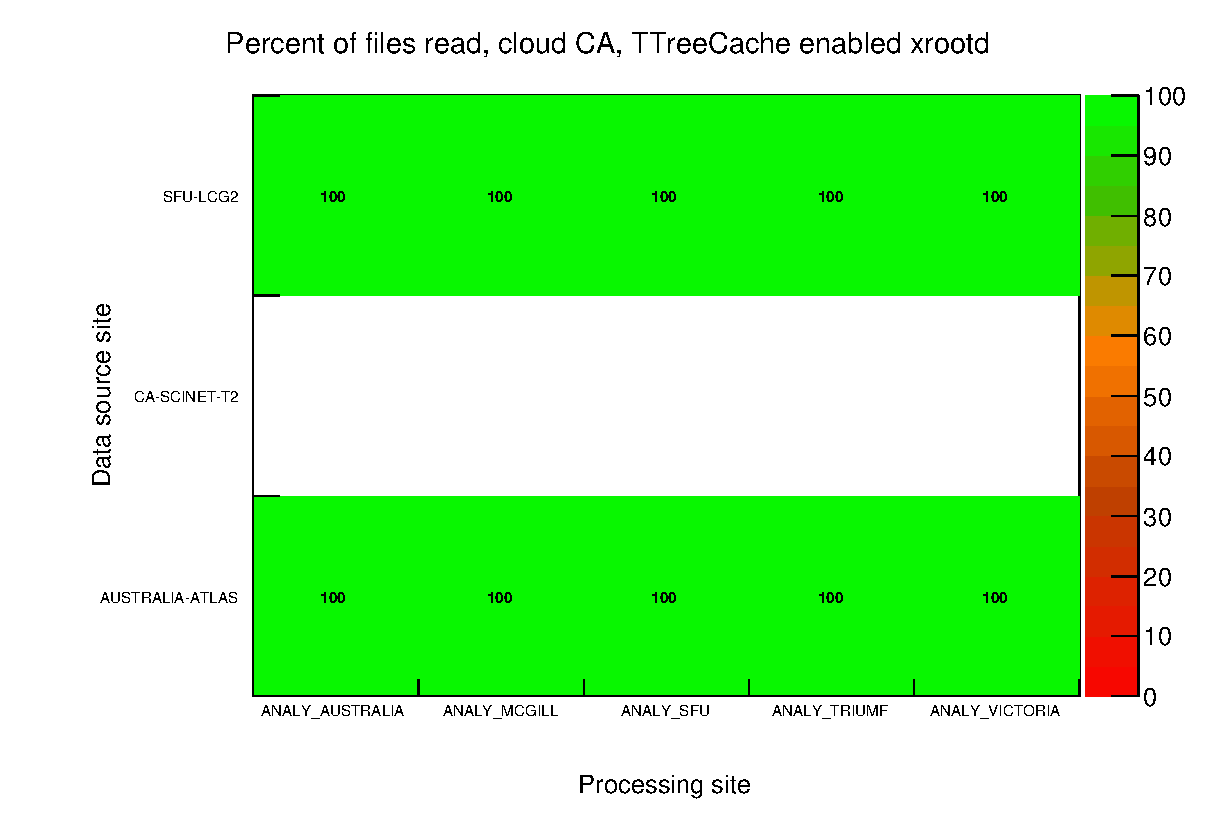
\includegraphics[width=\textwidth]{CA_xPerCentFile.eps}
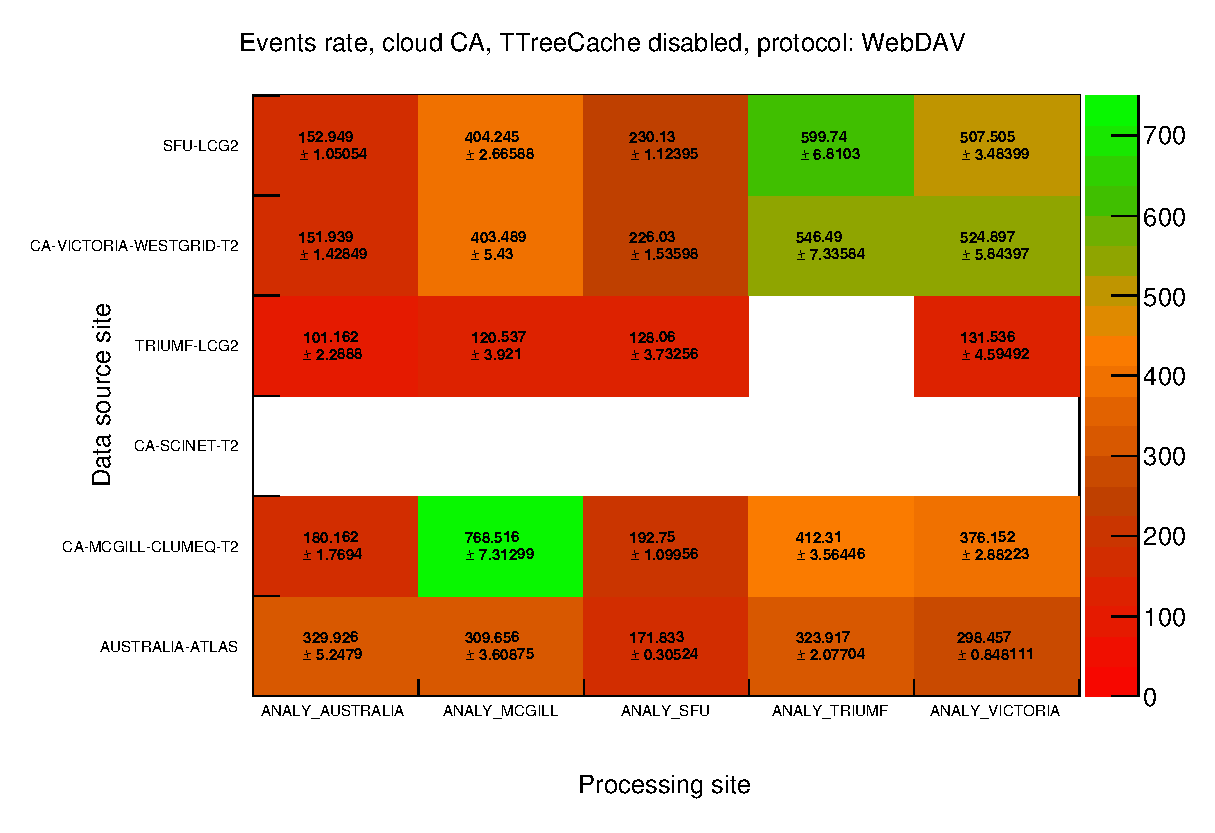
\includegraphics[width=\textwidth]{CA_EventsRate.eps}
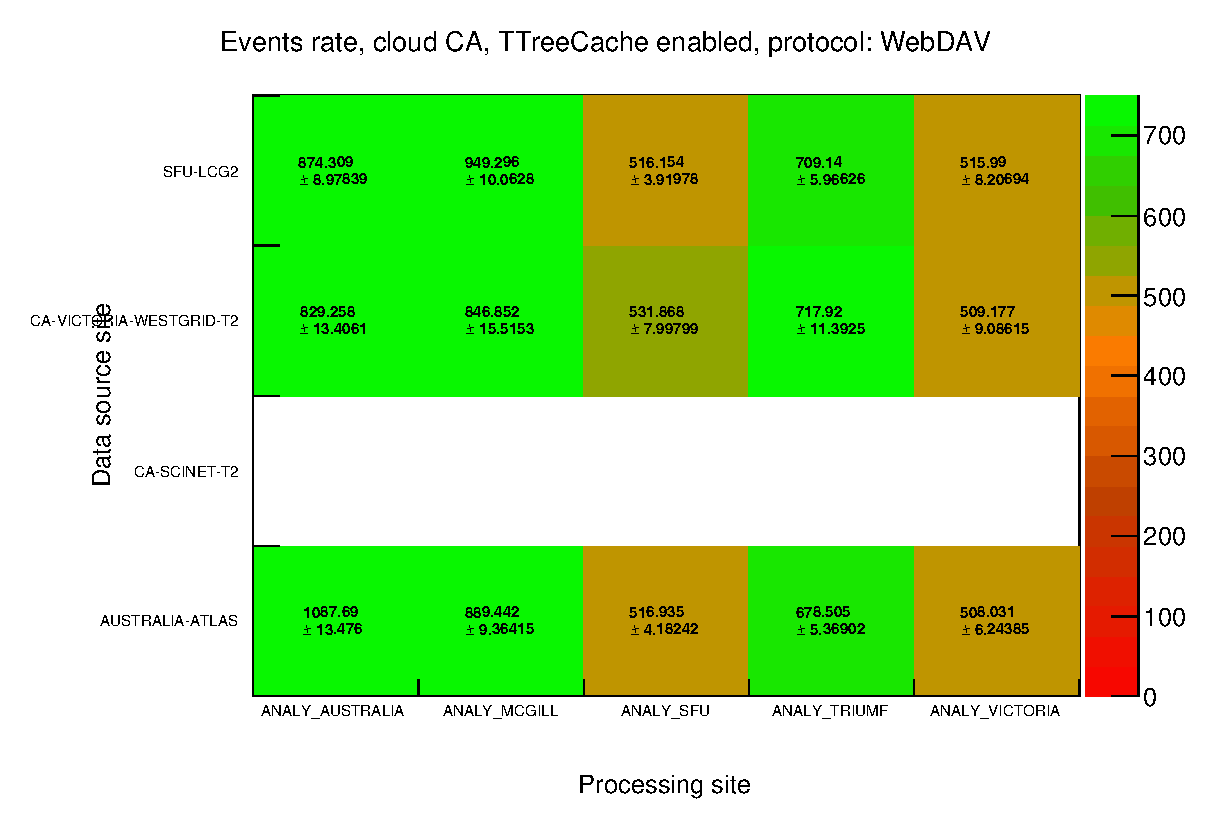
\includegraphics[width=\textwidth]{CA_tEventsRate.eps}
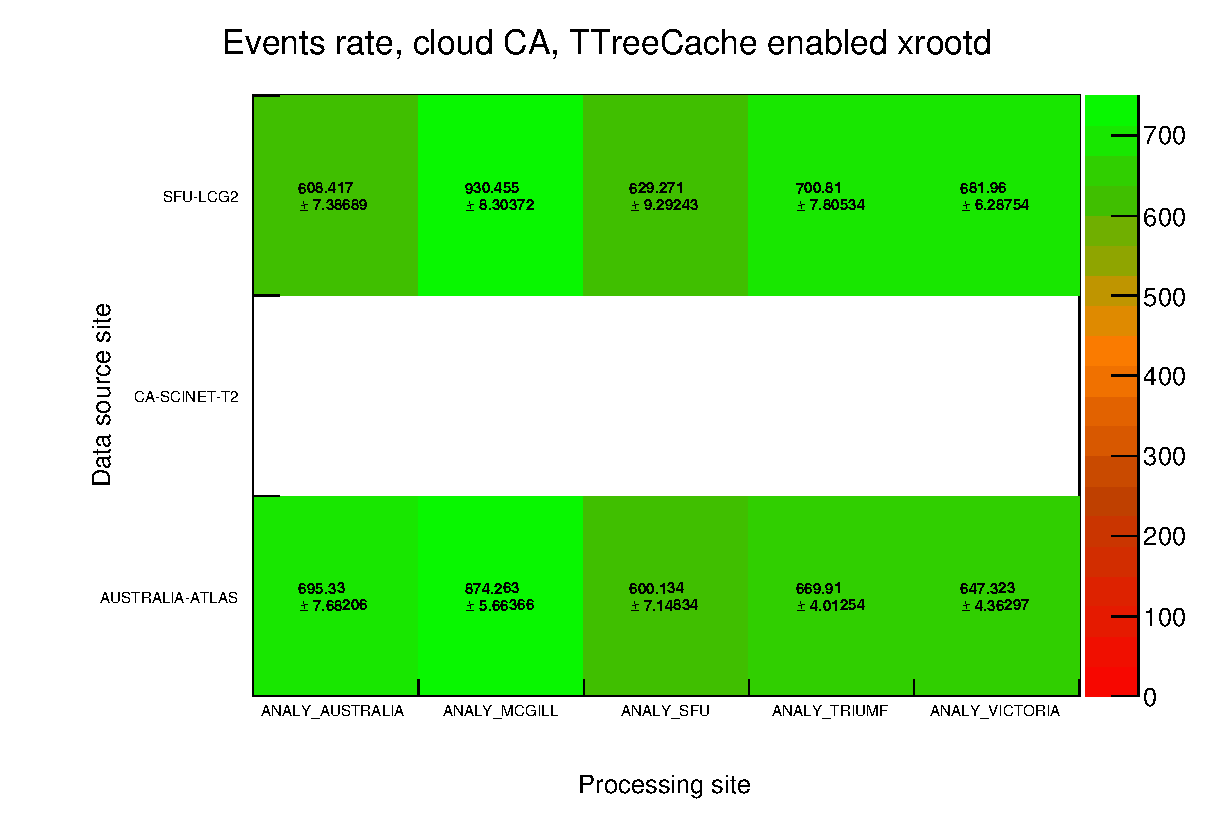
\includegraphics[width=\textwidth]{CA_xEventsRate.eps}
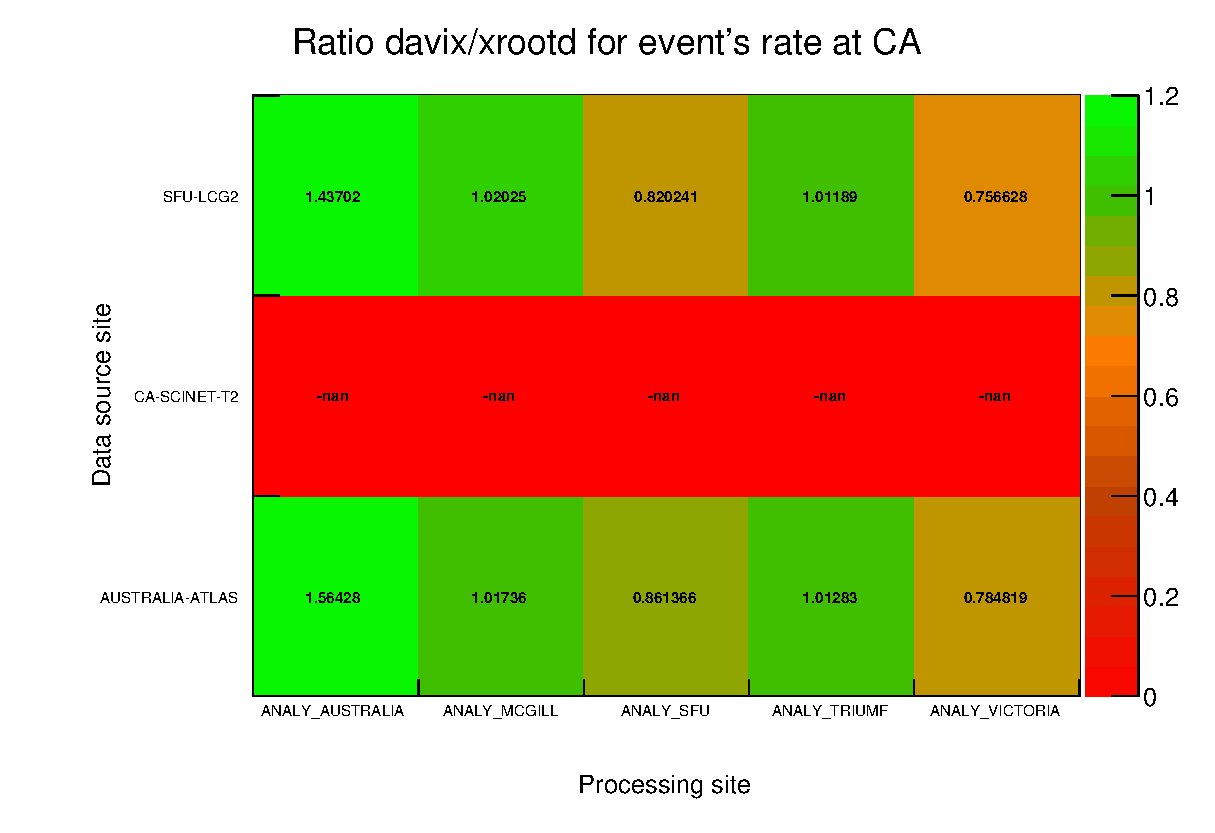
\includegraphics[width=\textwidth]{CA_xRatio.eps}
\vspace{1ex}\\

\subsection{Cloud DE}
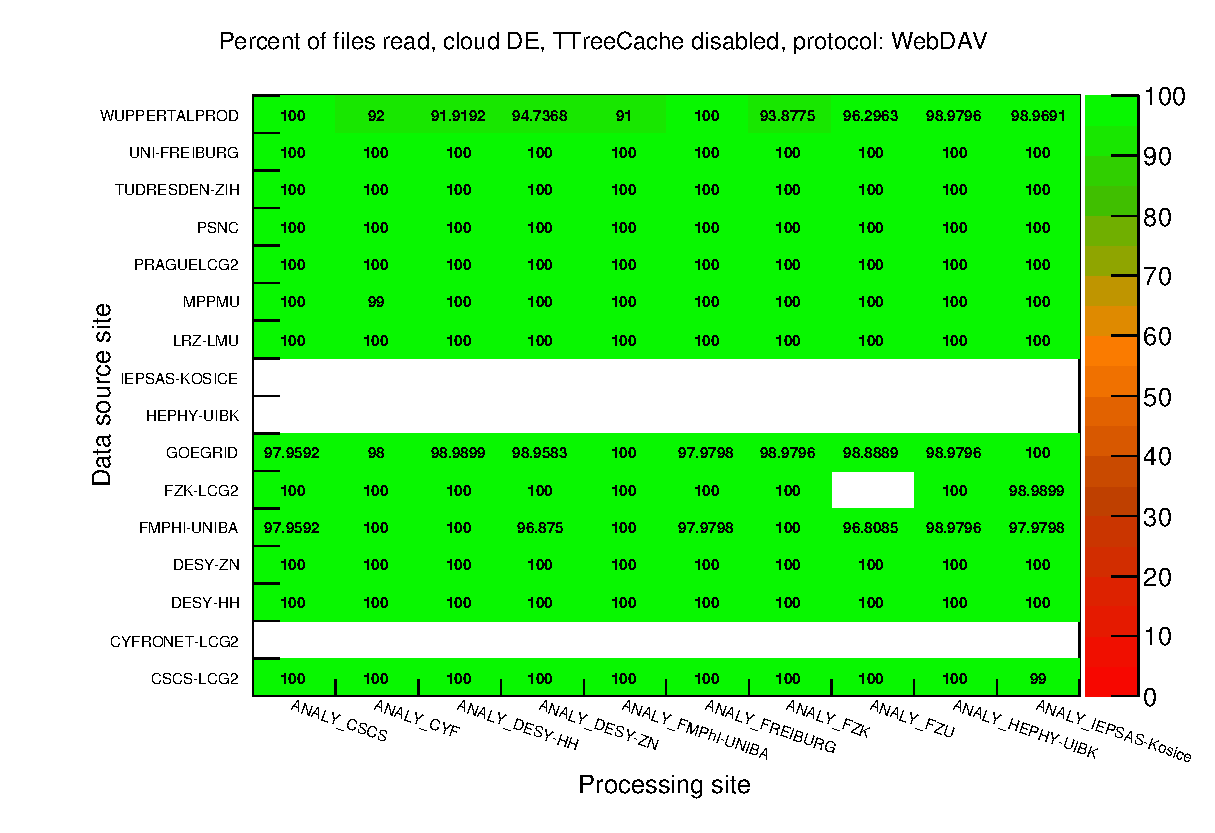
\includegraphics[width=\textwidth]{DE_PerCentFile.eps}
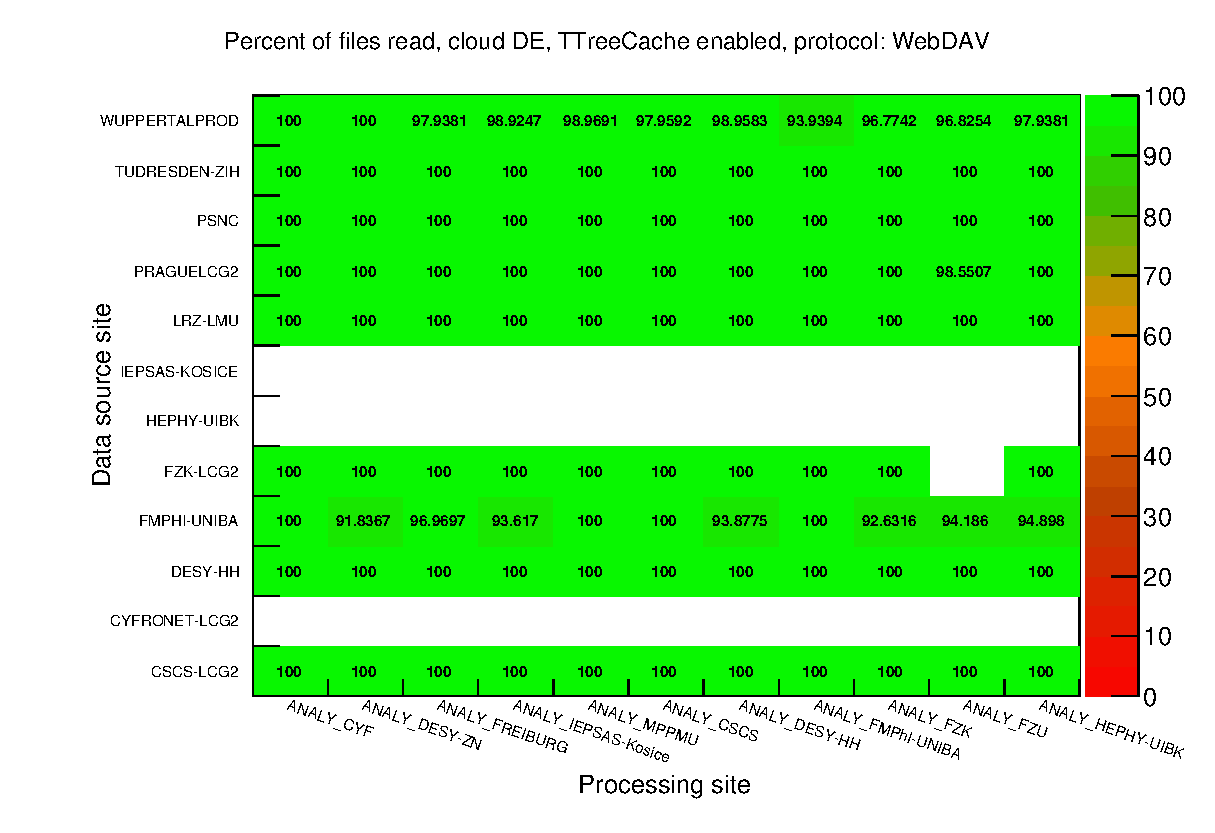
\includegraphics[width=\textwidth]{DE_tPerCentFile.eps}
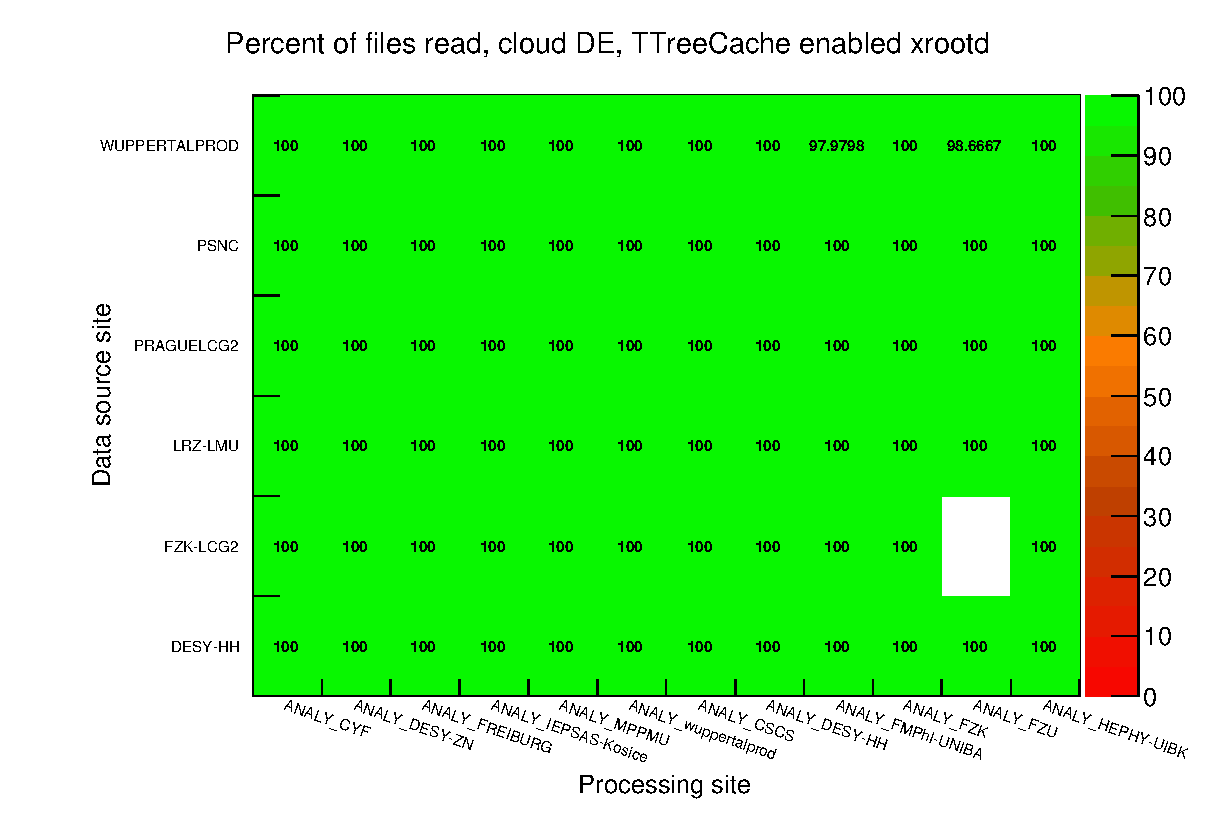
\includegraphics[width=\textwidth]{DE_xPerCentFile.eps}
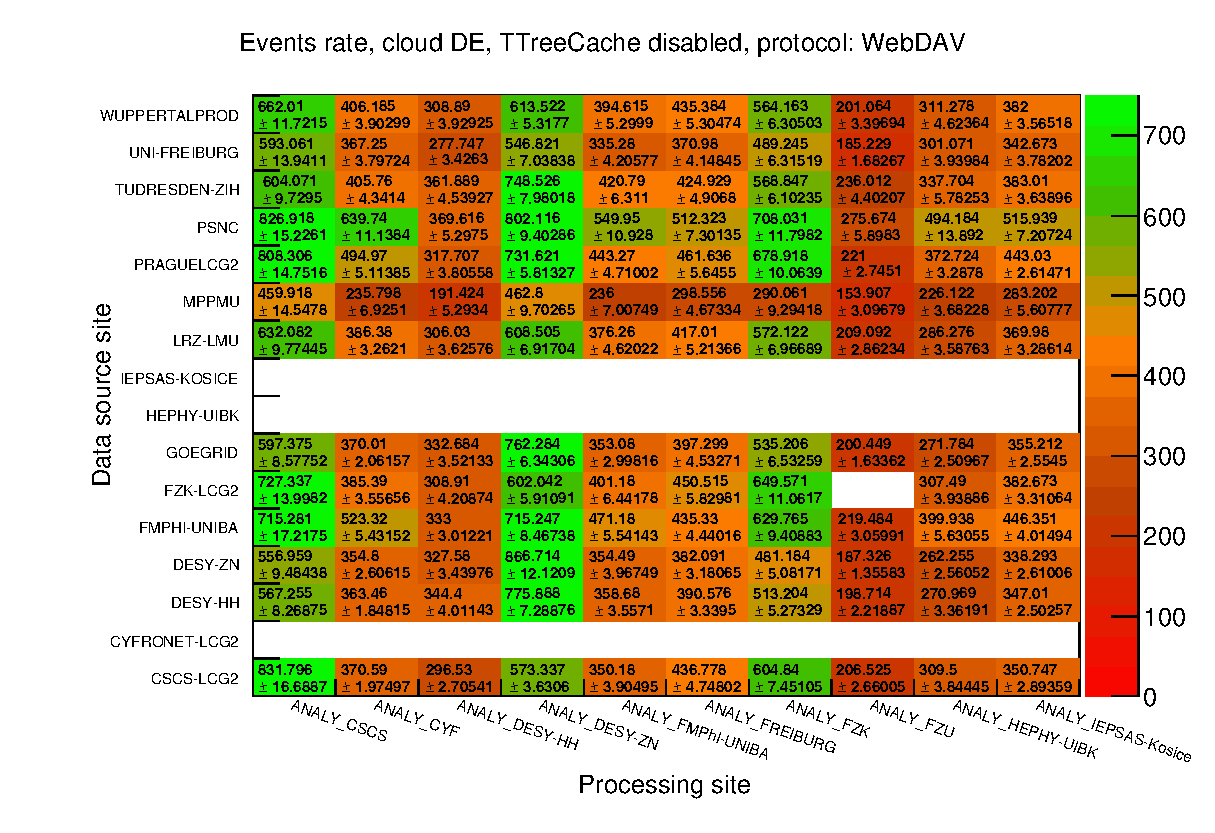
\includegraphics[width=\textwidth]{DE_EventsRate.eps}
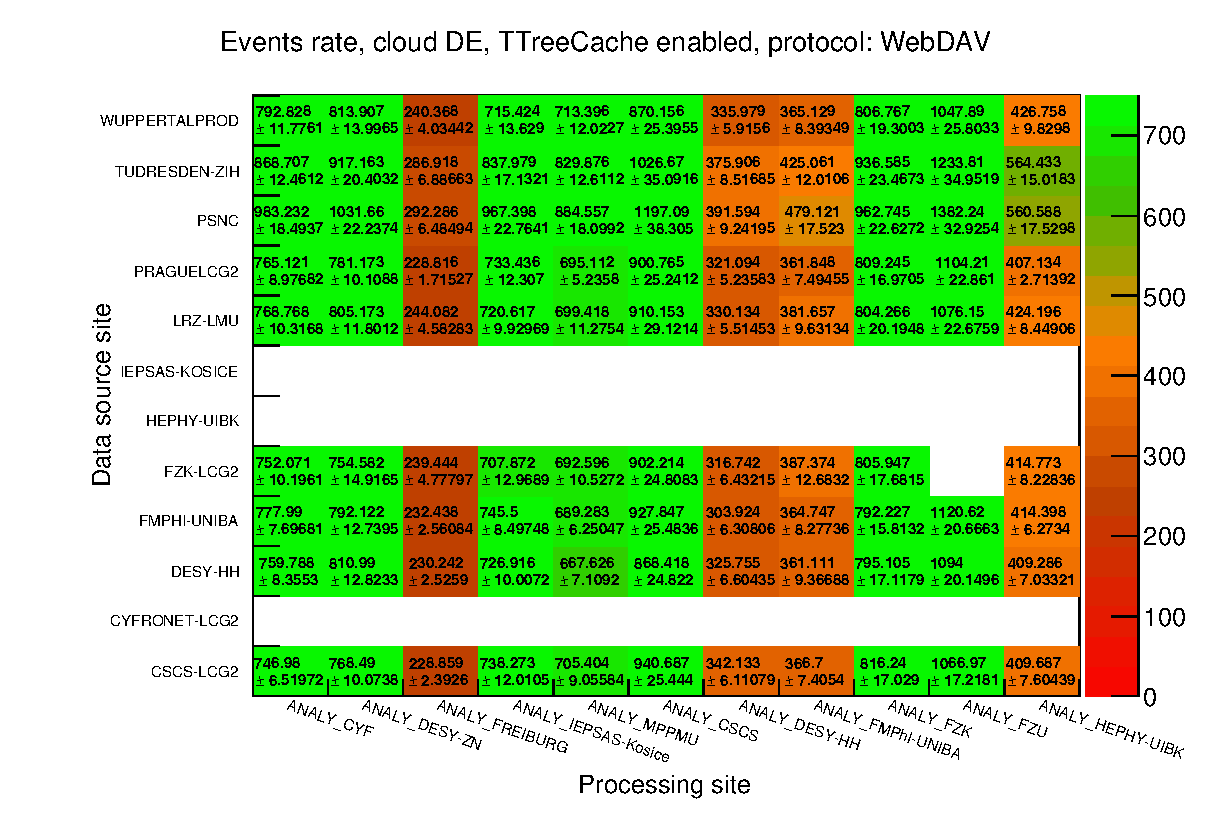
\includegraphics[width=\textwidth]{DE_tEventsRate.eps}
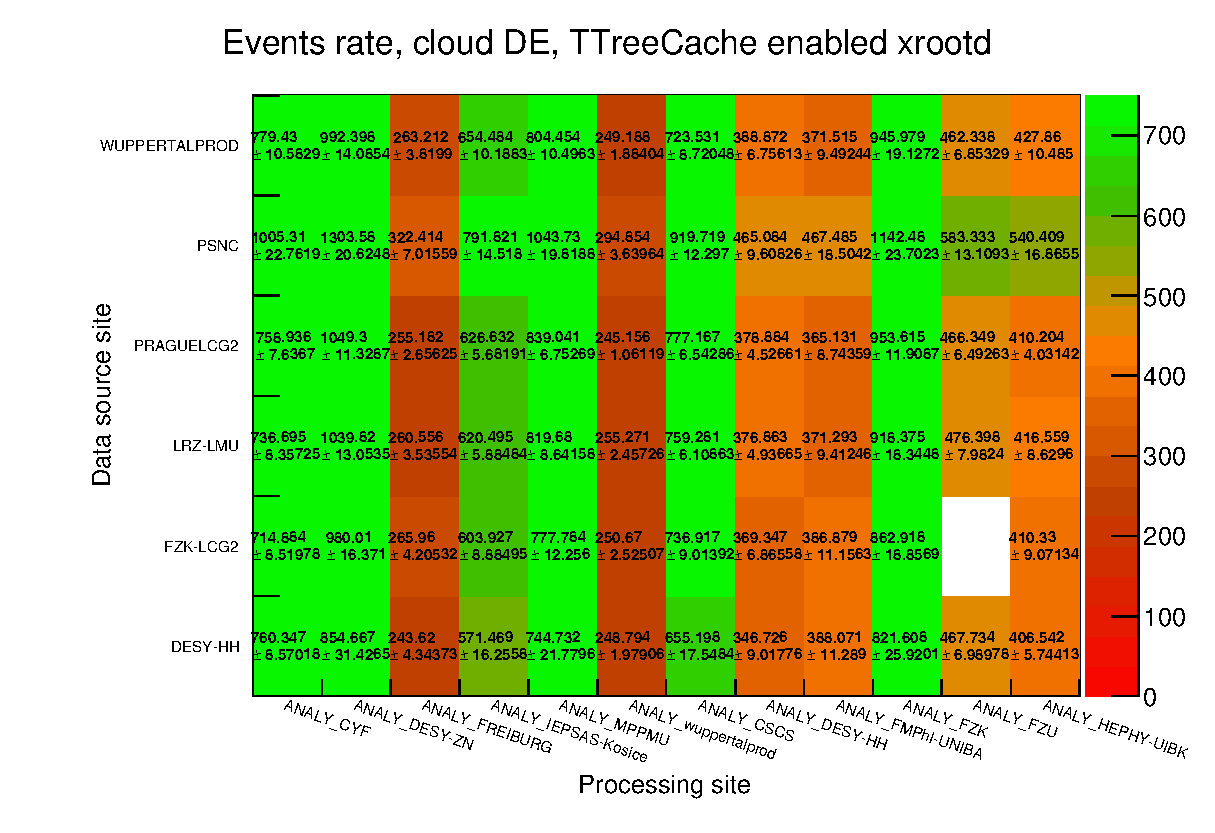
\includegraphics[width=\textwidth]{DE_xEventsRate.eps}
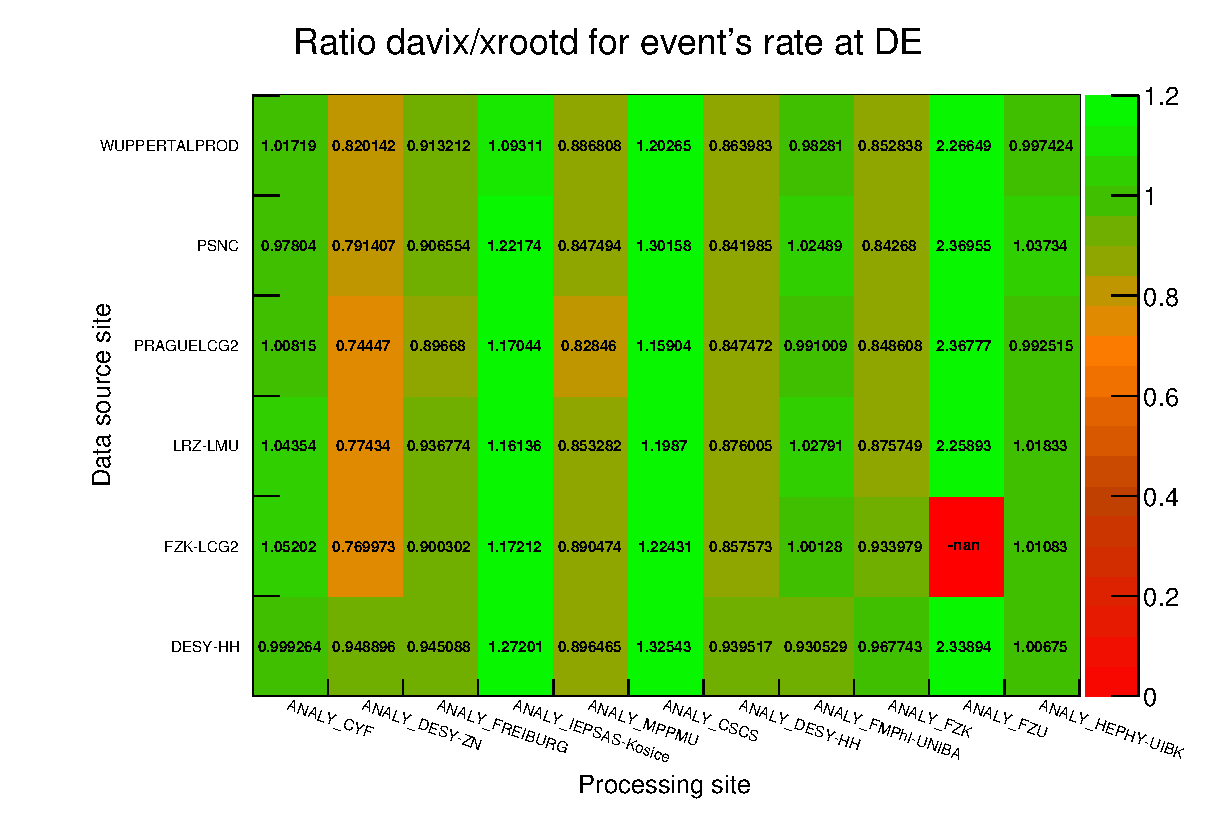
\includegraphics[width=\textwidth]{DE_xRatio.eps}
\vspace{1ex}\\

\subsection{Cloud ES}
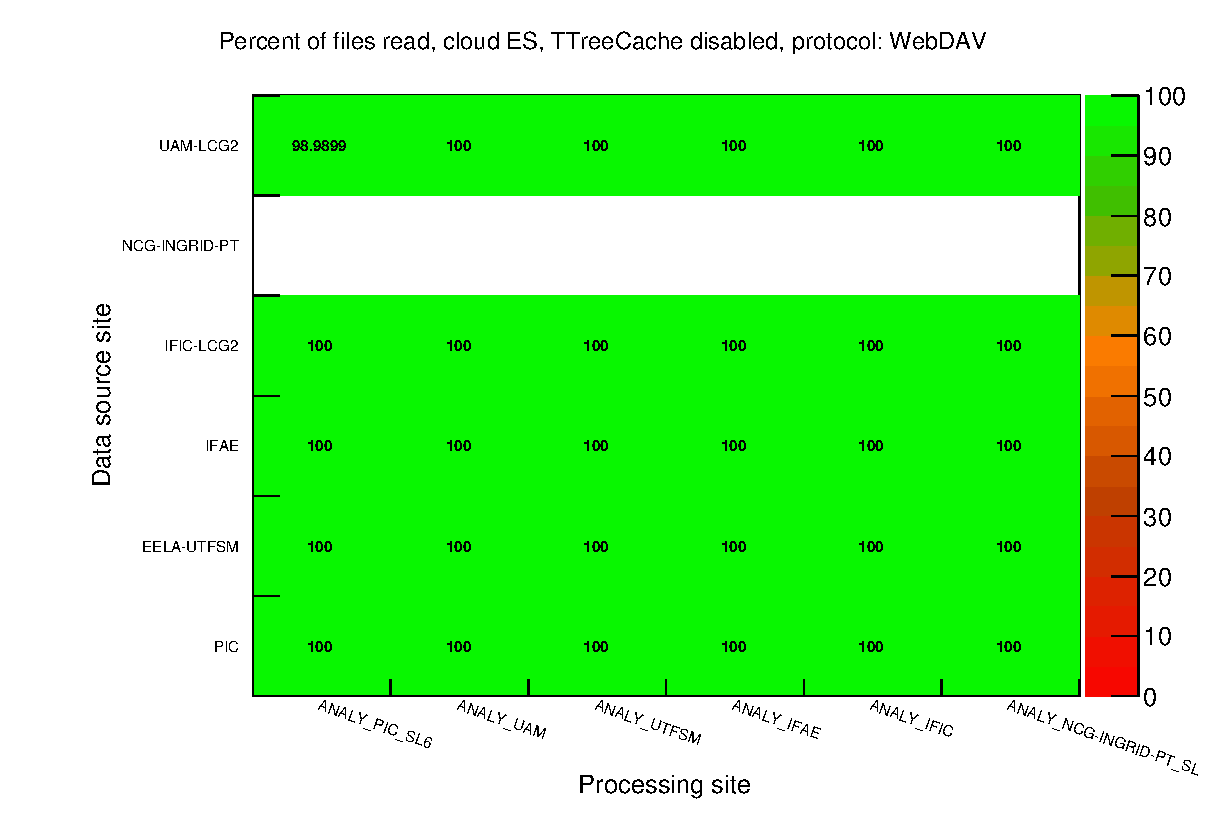
\includegraphics[width=\textwidth]{ES_PerCentFile.eps}
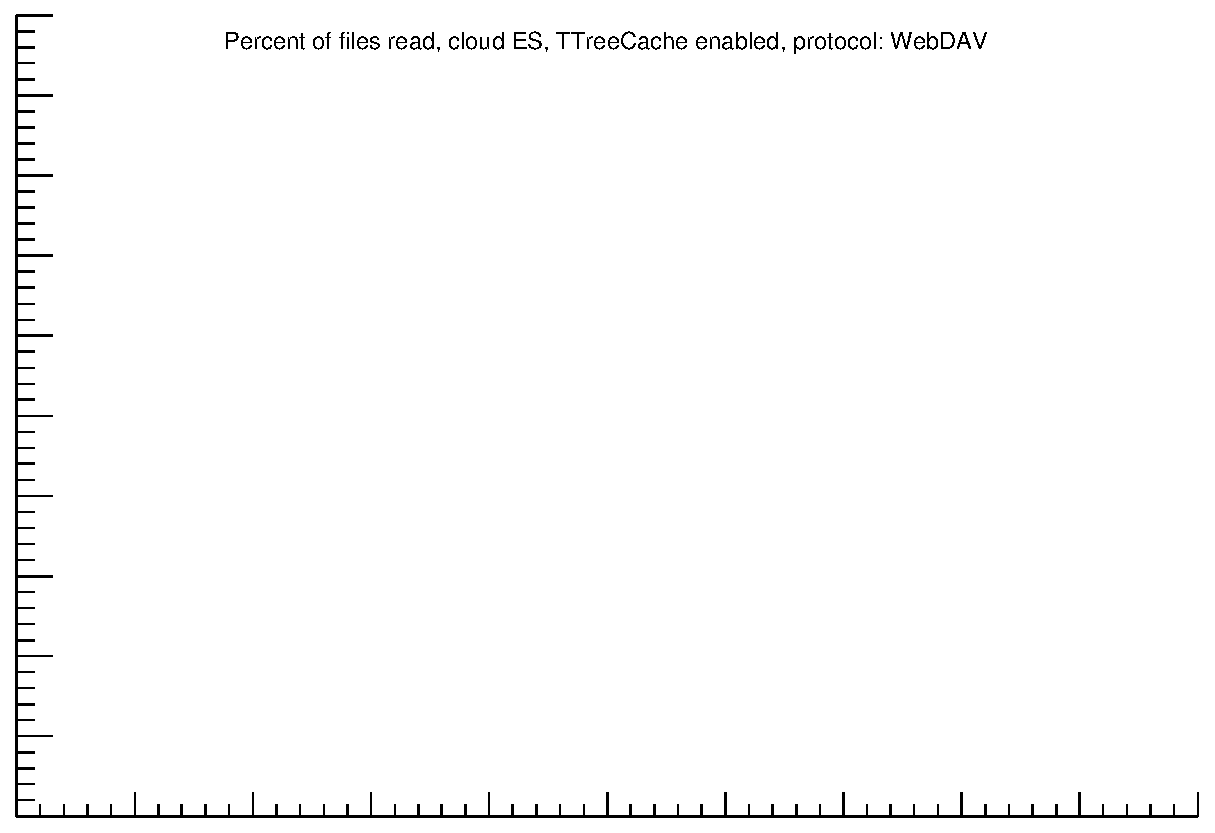
\includegraphics[width=\textwidth]{ES_tPerCentFile.eps}
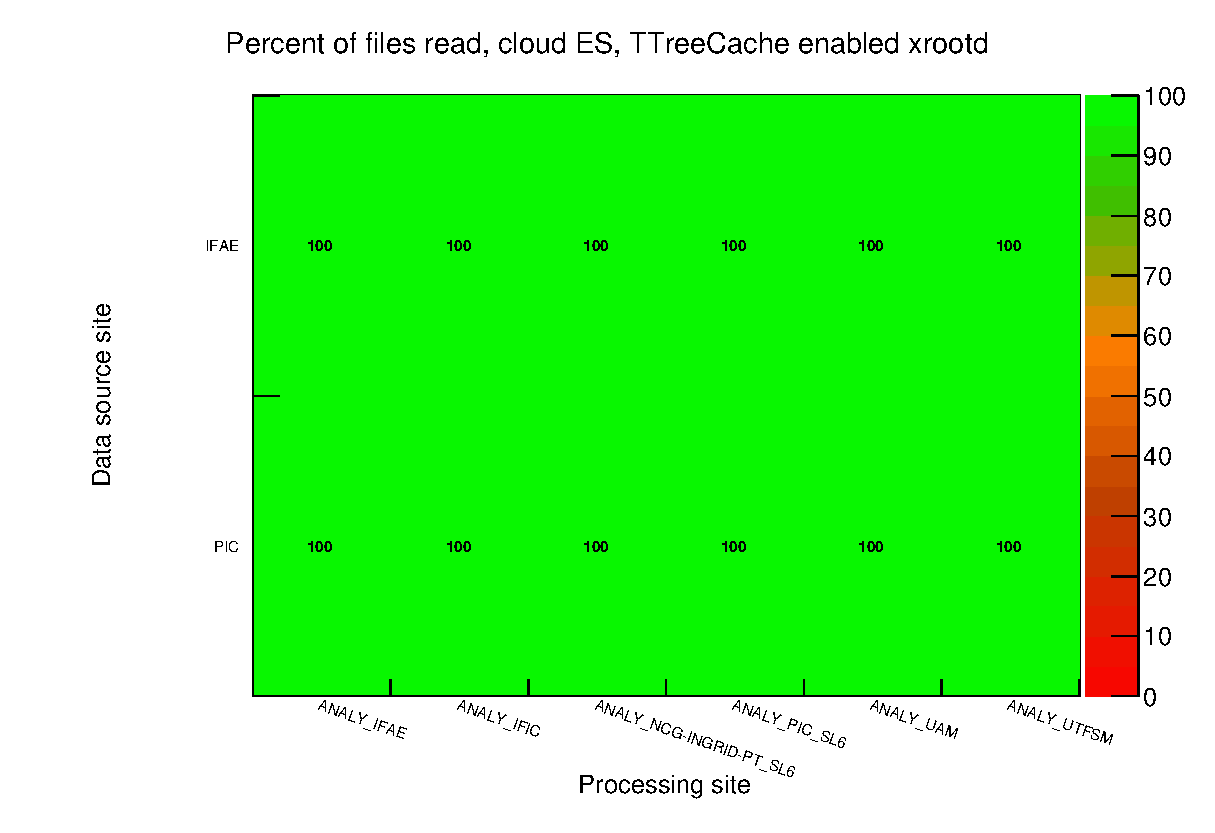
\includegraphics[width=\textwidth]{ES_xPerCentFile.eps}
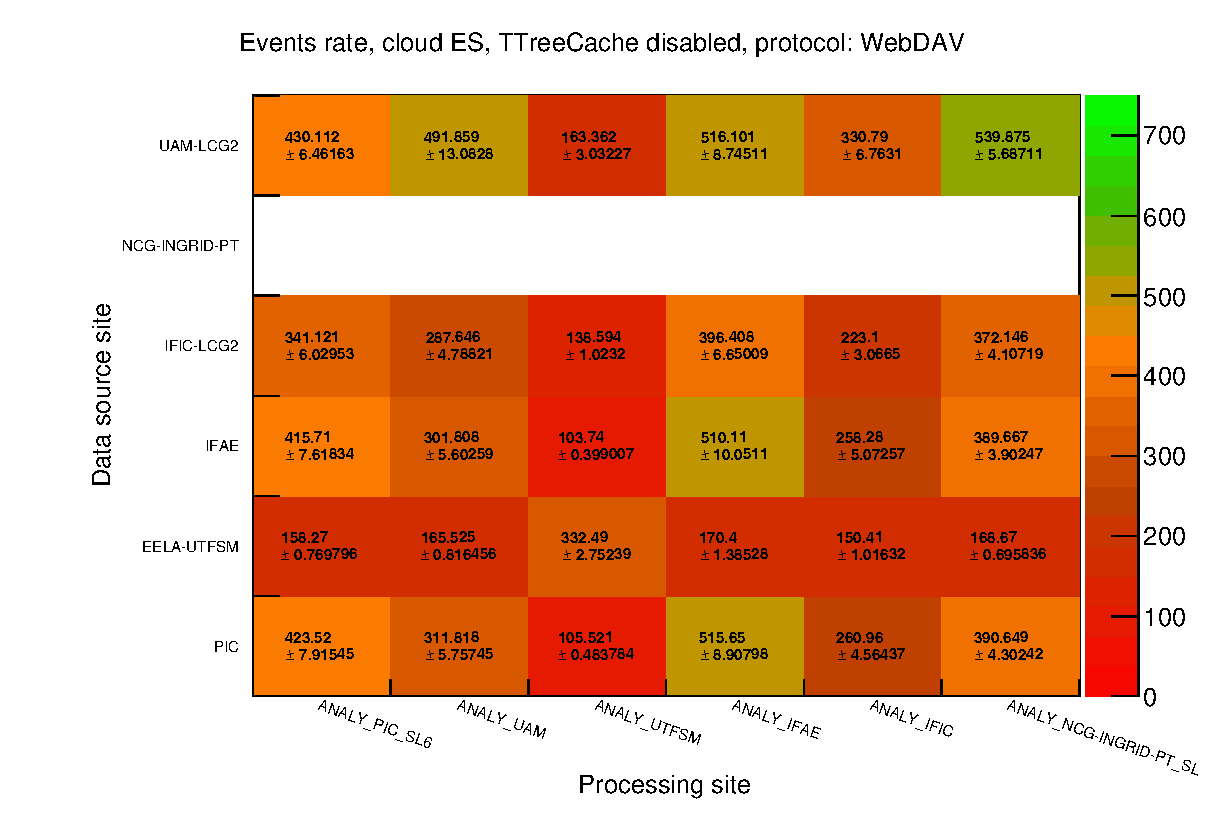
\includegraphics[width=\textwidth]{ES_EventsRate.eps}
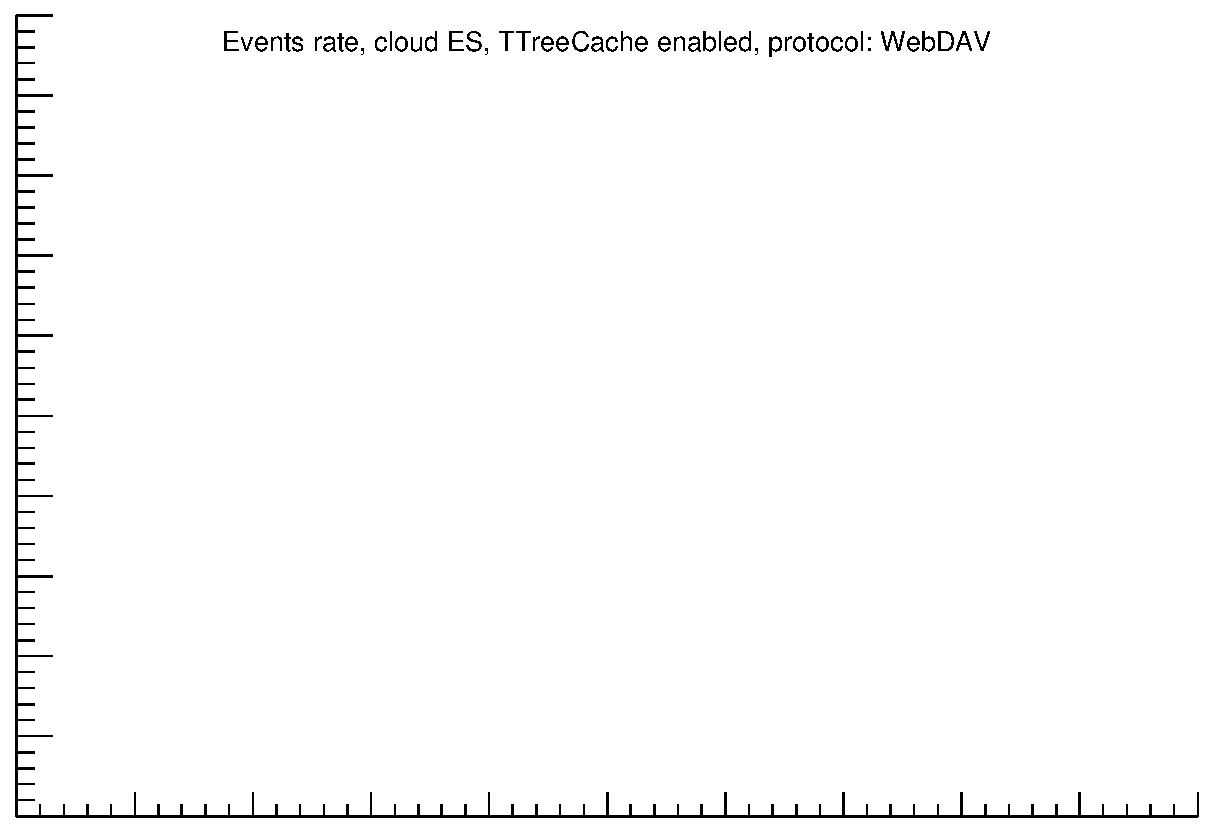
\includegraphics[width=\textwidth]{ES_tEventsRate.eps}
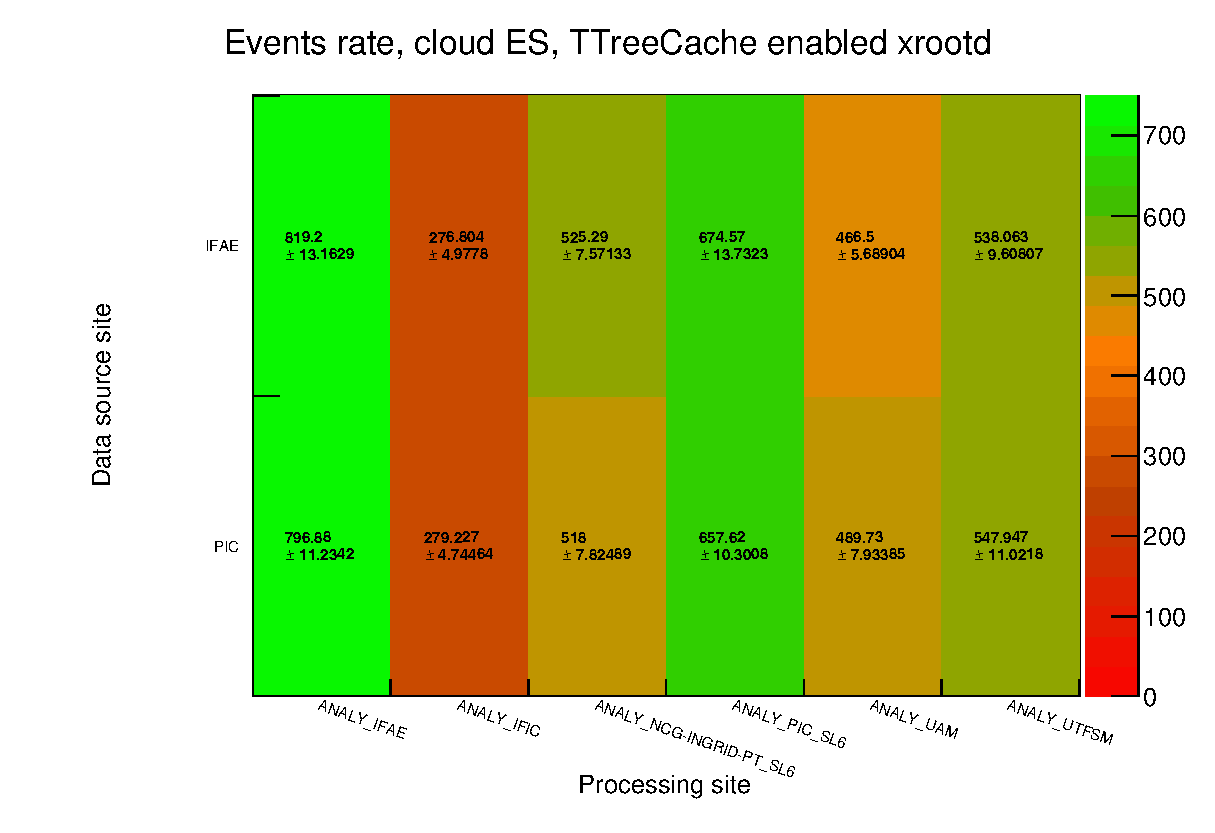
\includegraphics[width=\textwidth]{ES_xEventsRate.eps}
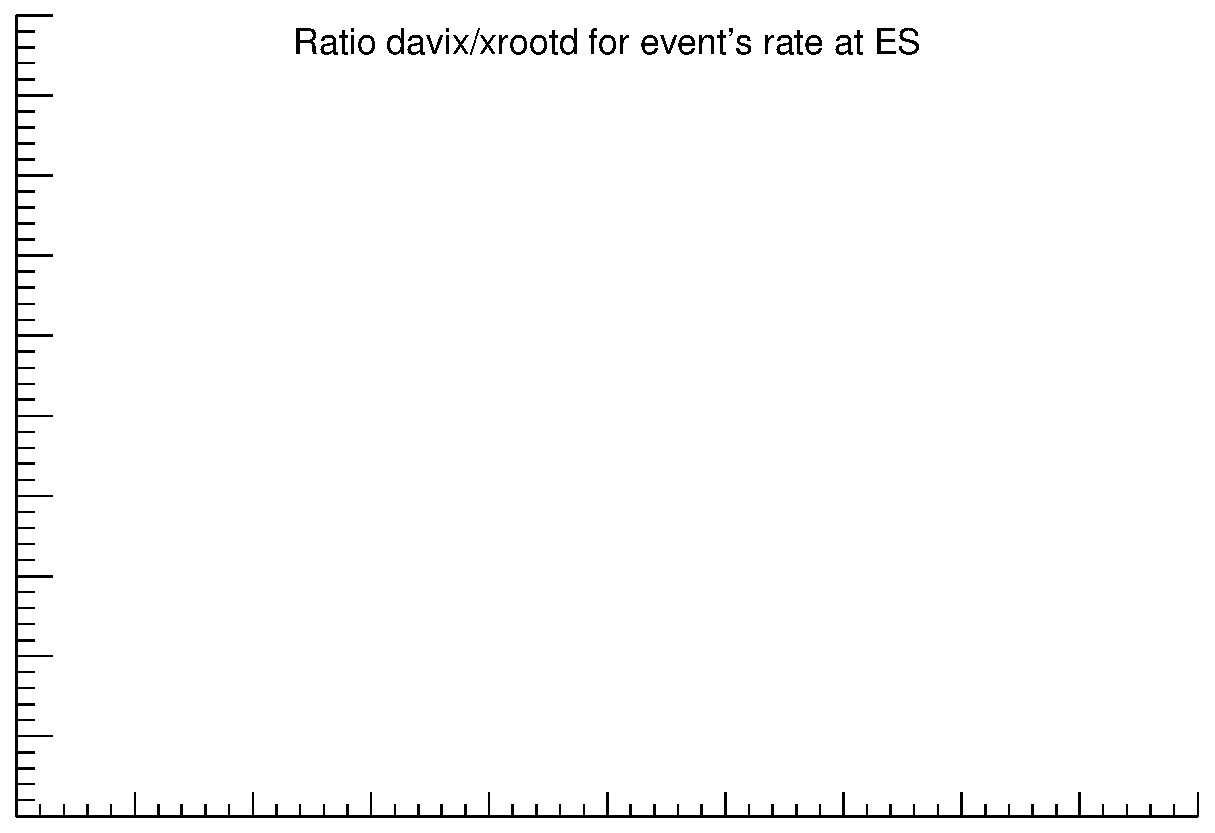
\includegraphics[width=\textwidth]{ES_xRatio.eps}
\vspace{1ex}\\

\subsection{Cloud FR}
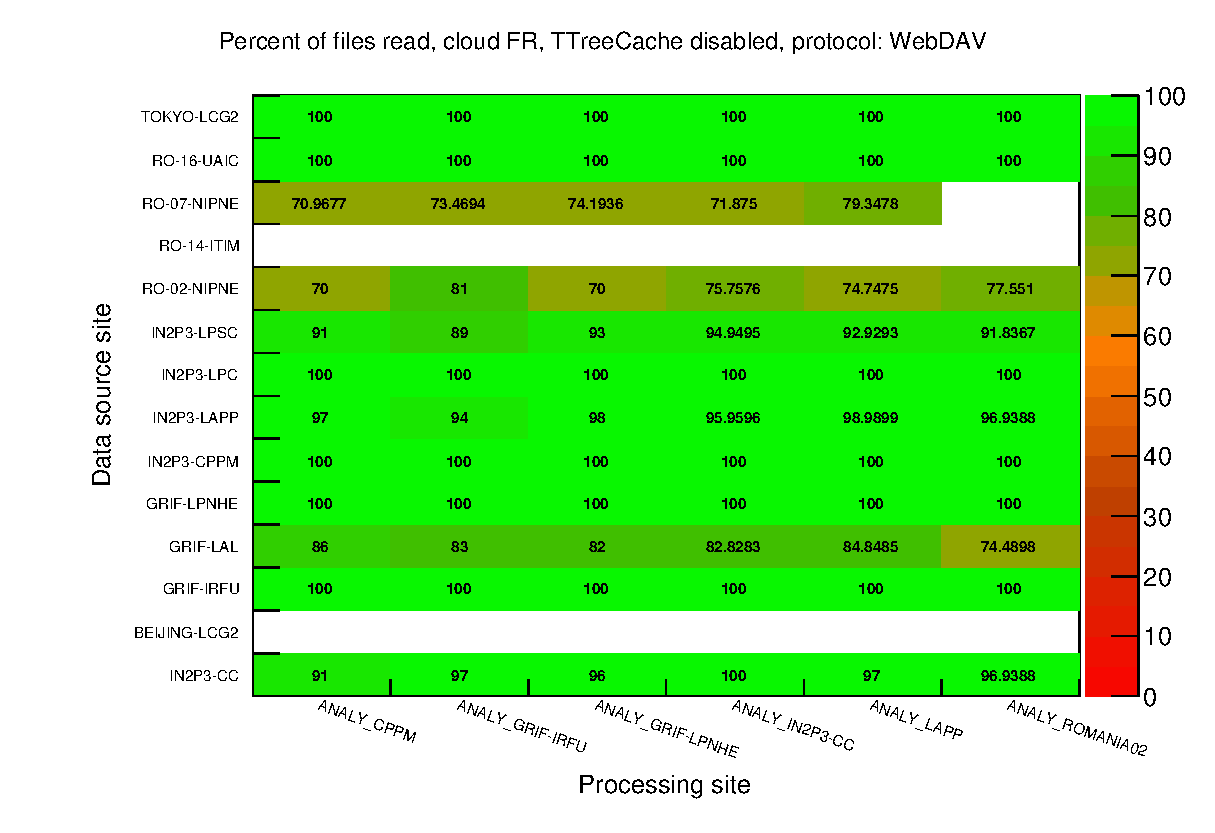
\includegraphics[width=\textwidth]{FR_PerCentFile.eps}
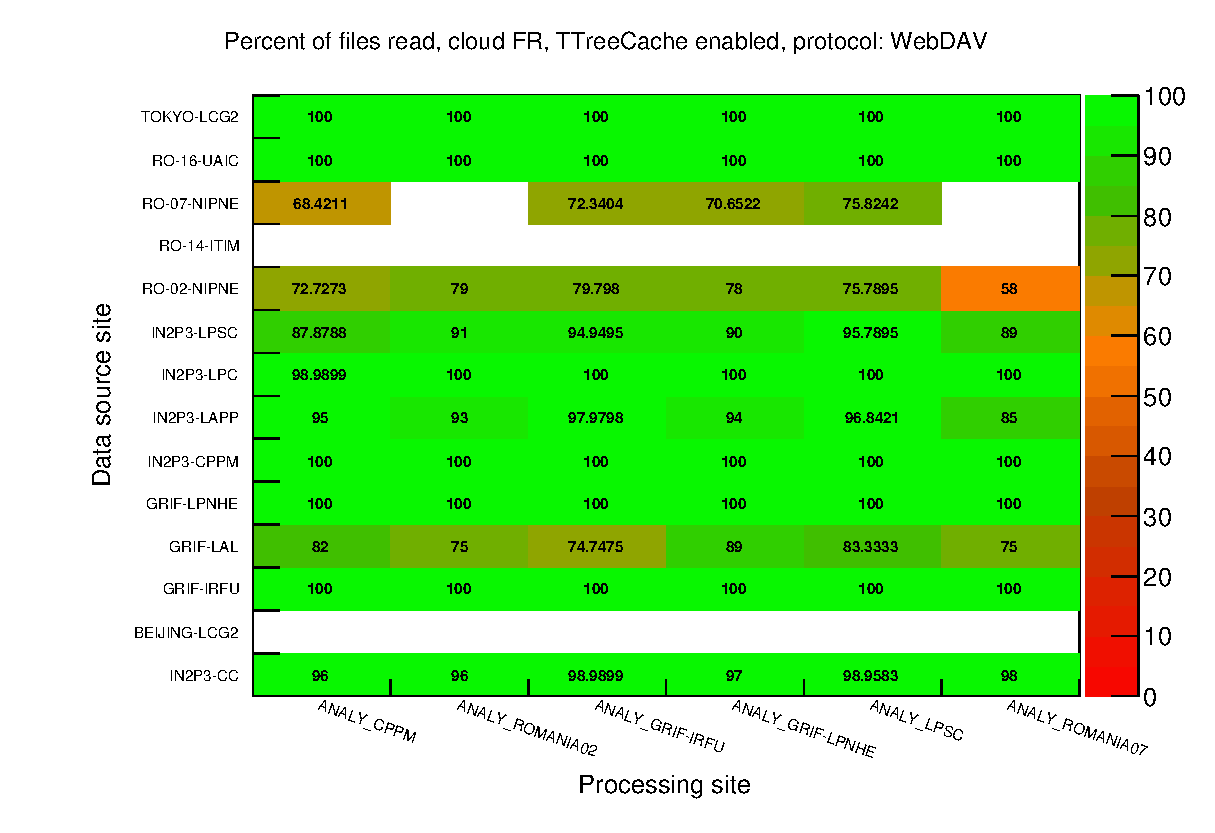
\includegraphics[width=\textwidth]{FR_tPerCentFile.eps}
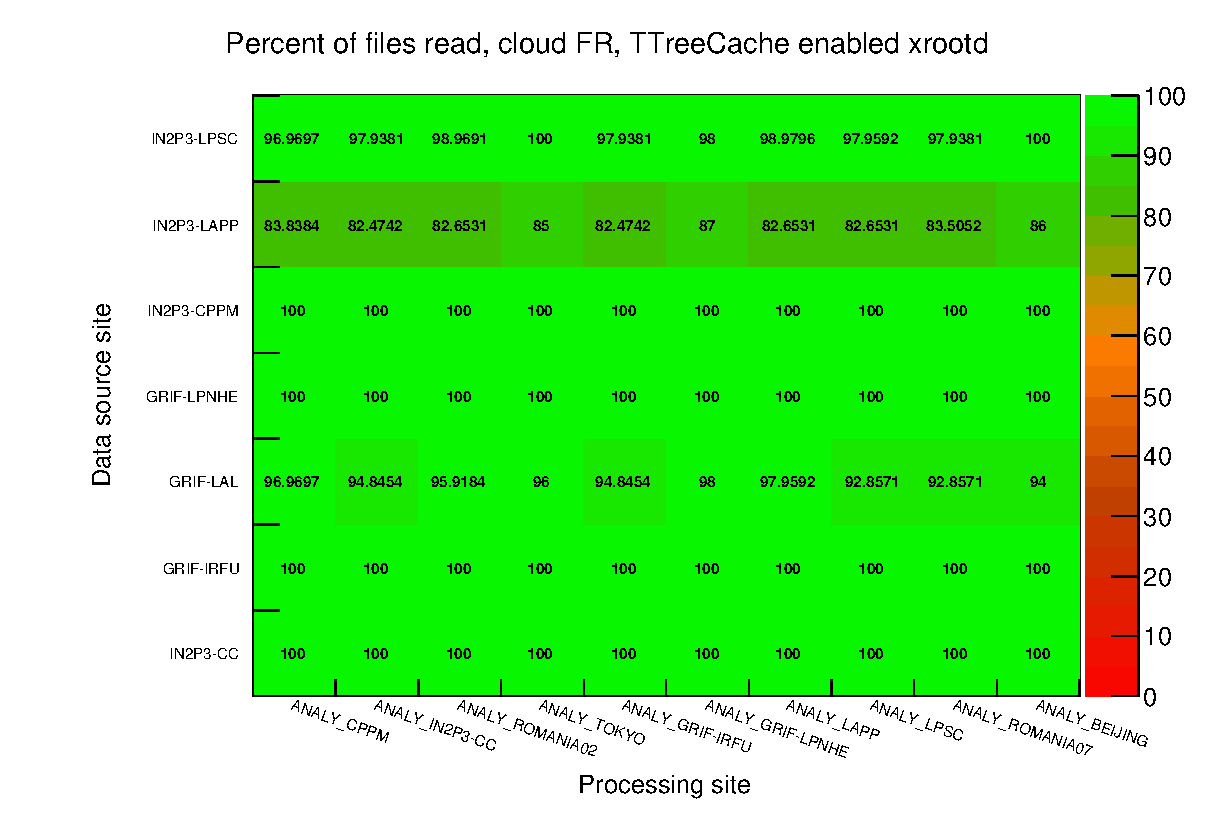
\includegraphics[width=\textwidth]{FR_xPerCentFile.eps}
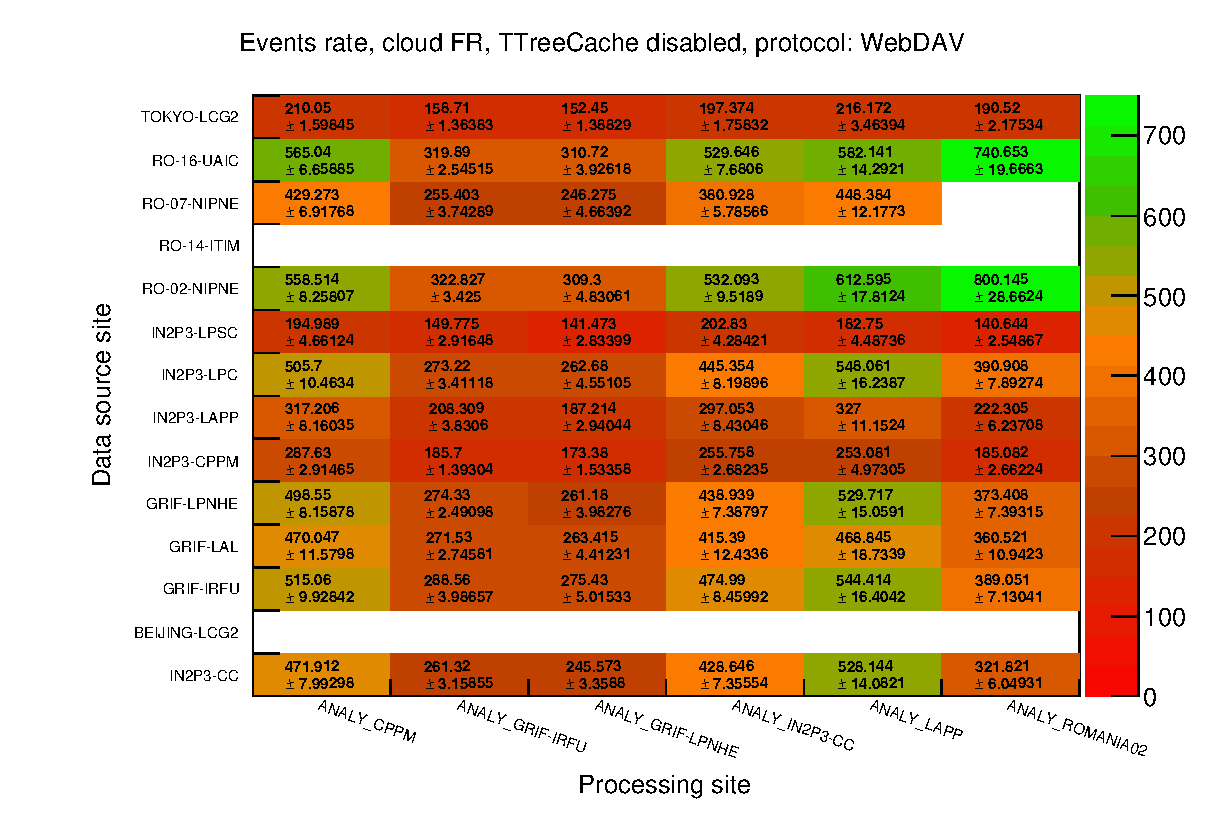
\includegraphics[width=\textwidth]{FR_EventsRate.eps}
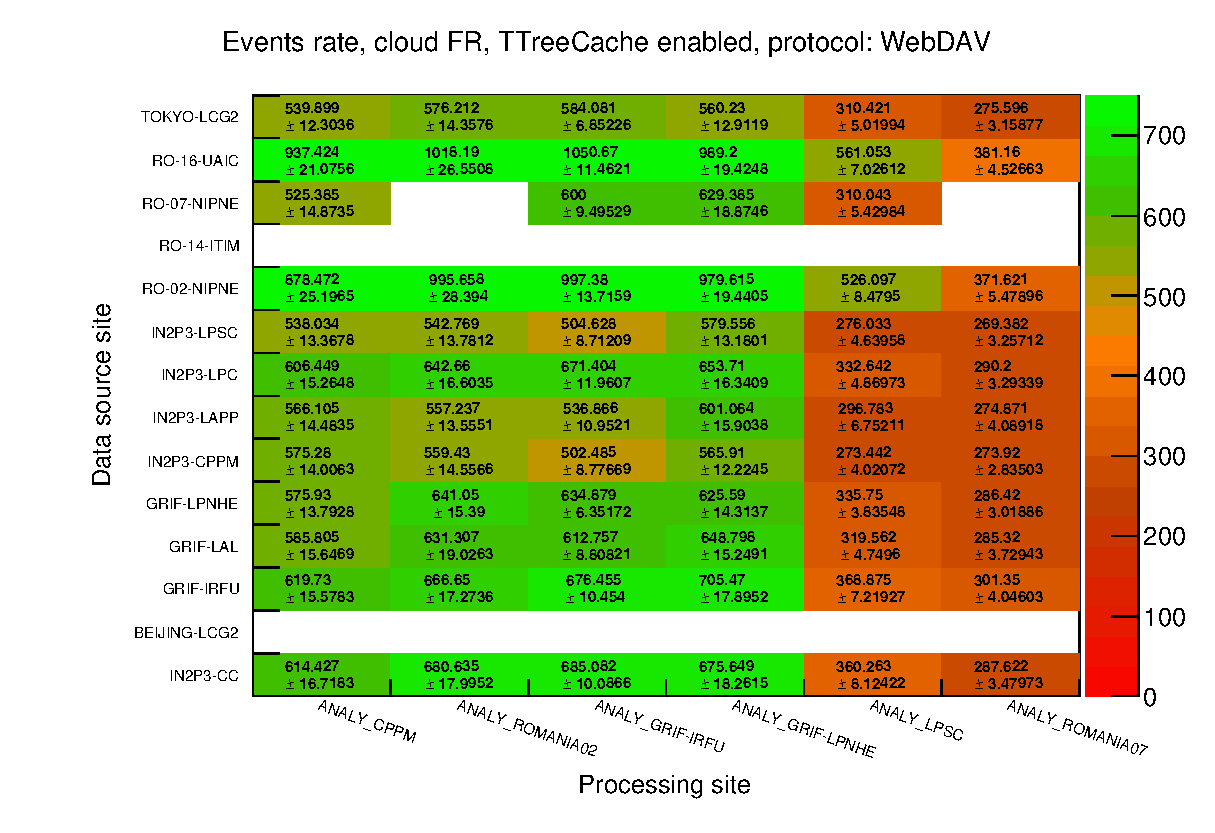
\includegraphics[width=\textwidth]{FR_tEventsRate.eps}
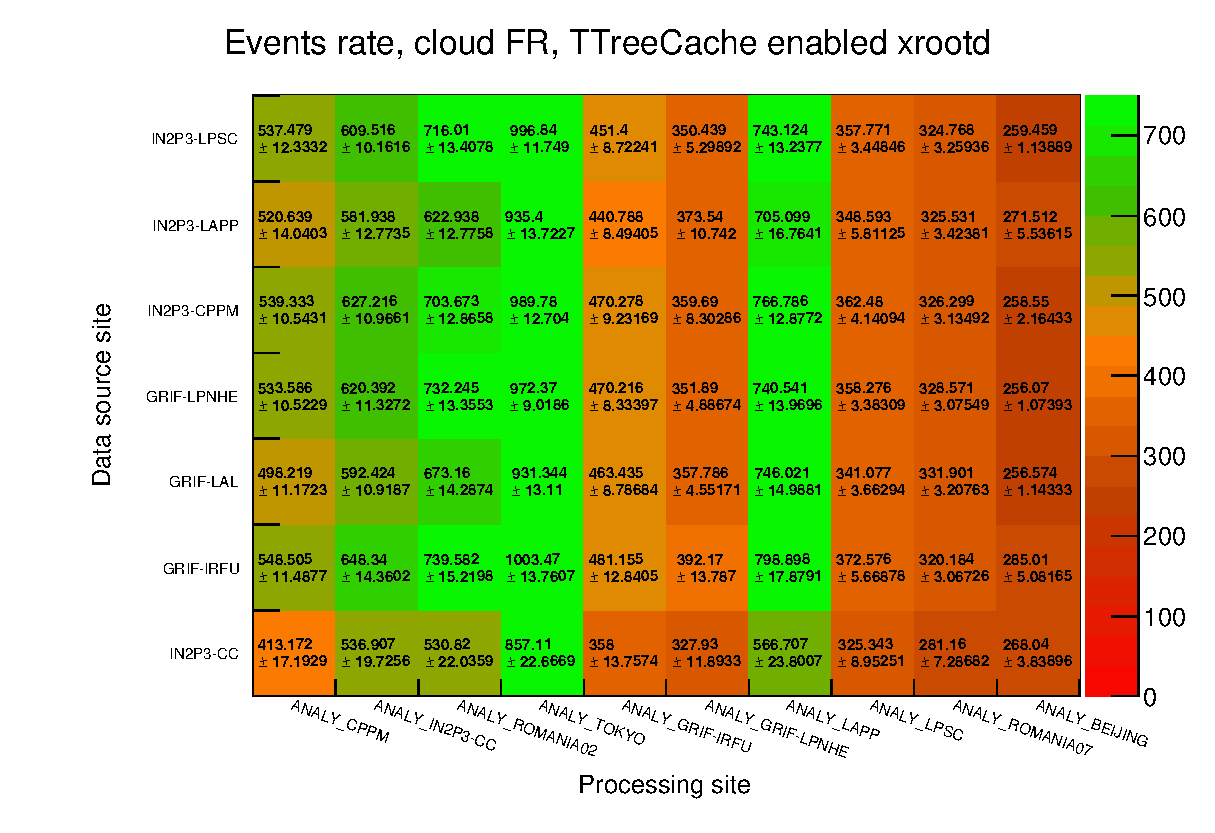
\includegraphics[width=\textwidth]{FR_xEventsRate.eps}
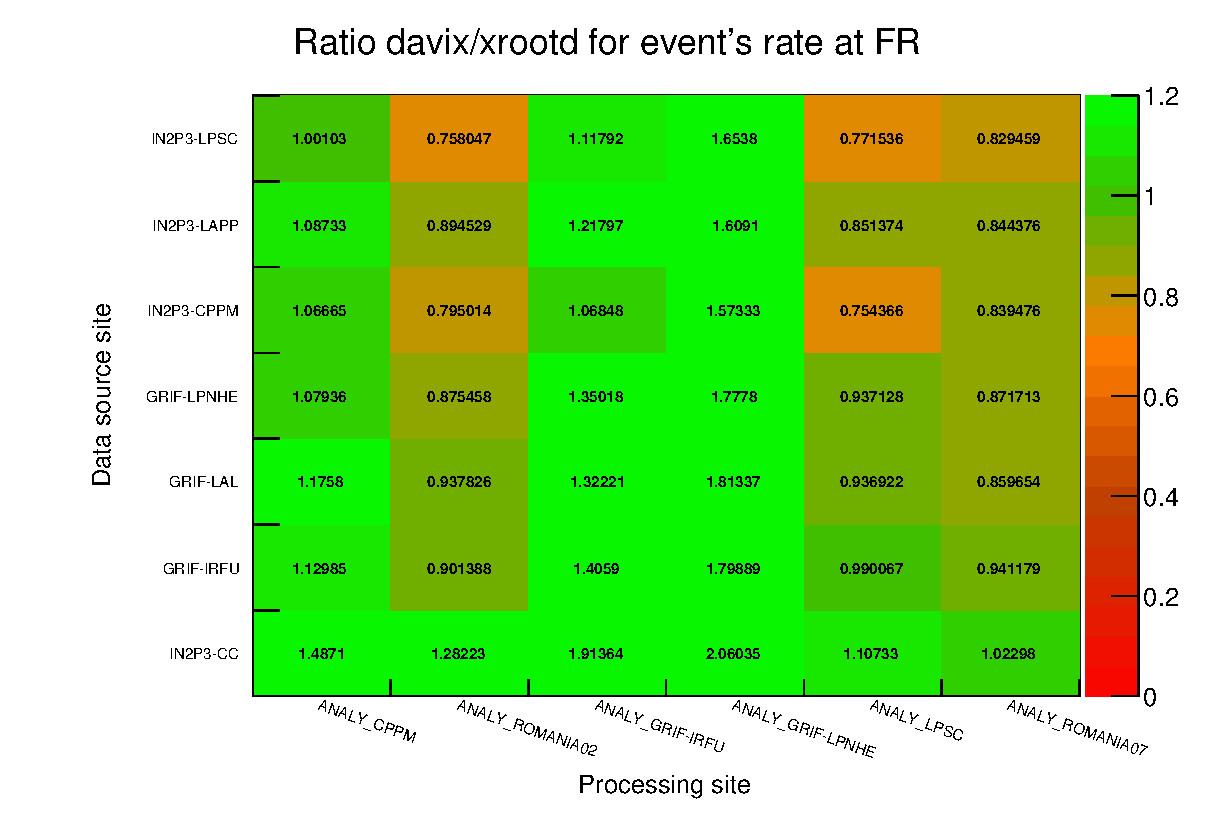
\includegraphics[width=\textwidth]{FR_xRatio.eps}
\vspace{1ex}\\

\subsection{Cloud IT}
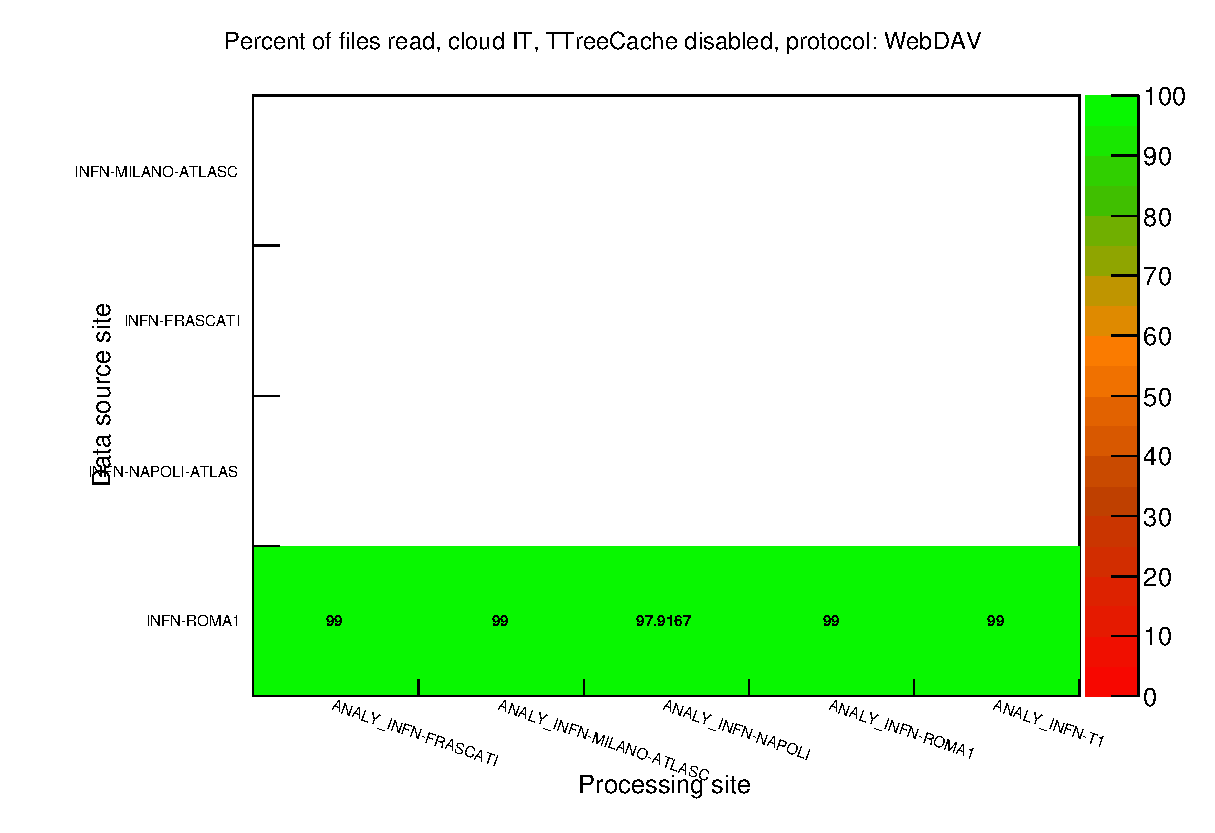
\includegraphics[width=\textwidth]{IT_PerCentFile.eps}
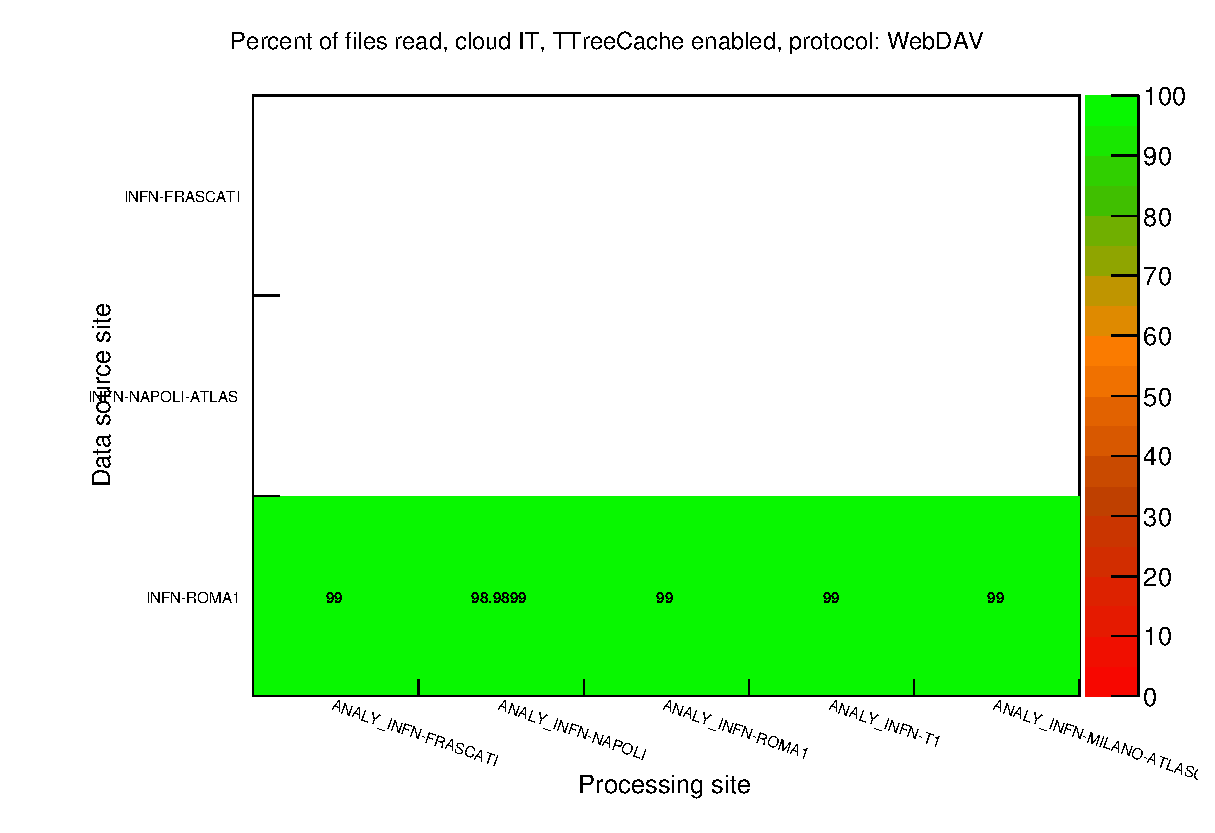
\includegraphics[width=\textwidth]{IT_tPerCentFile.eps}
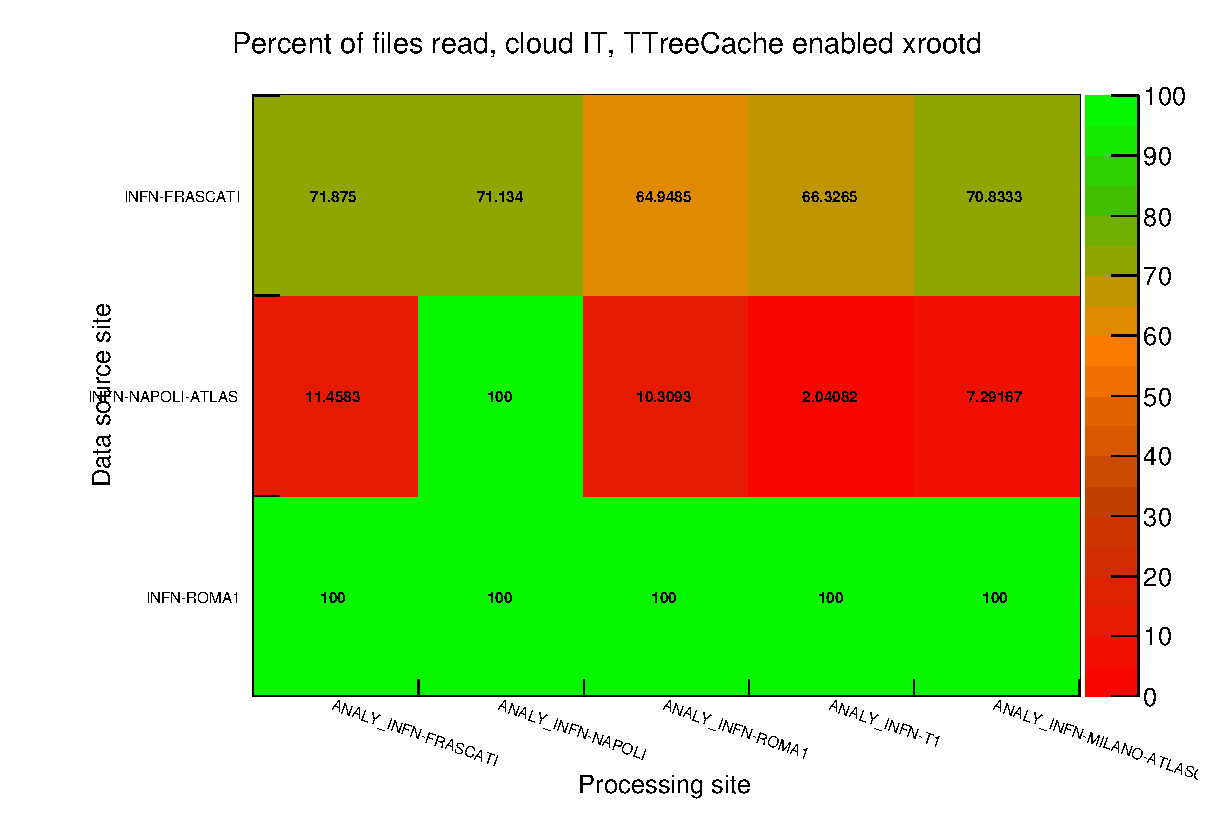
\includegraphics[width=\textwidth]{IT_xPerCentFile.eps}
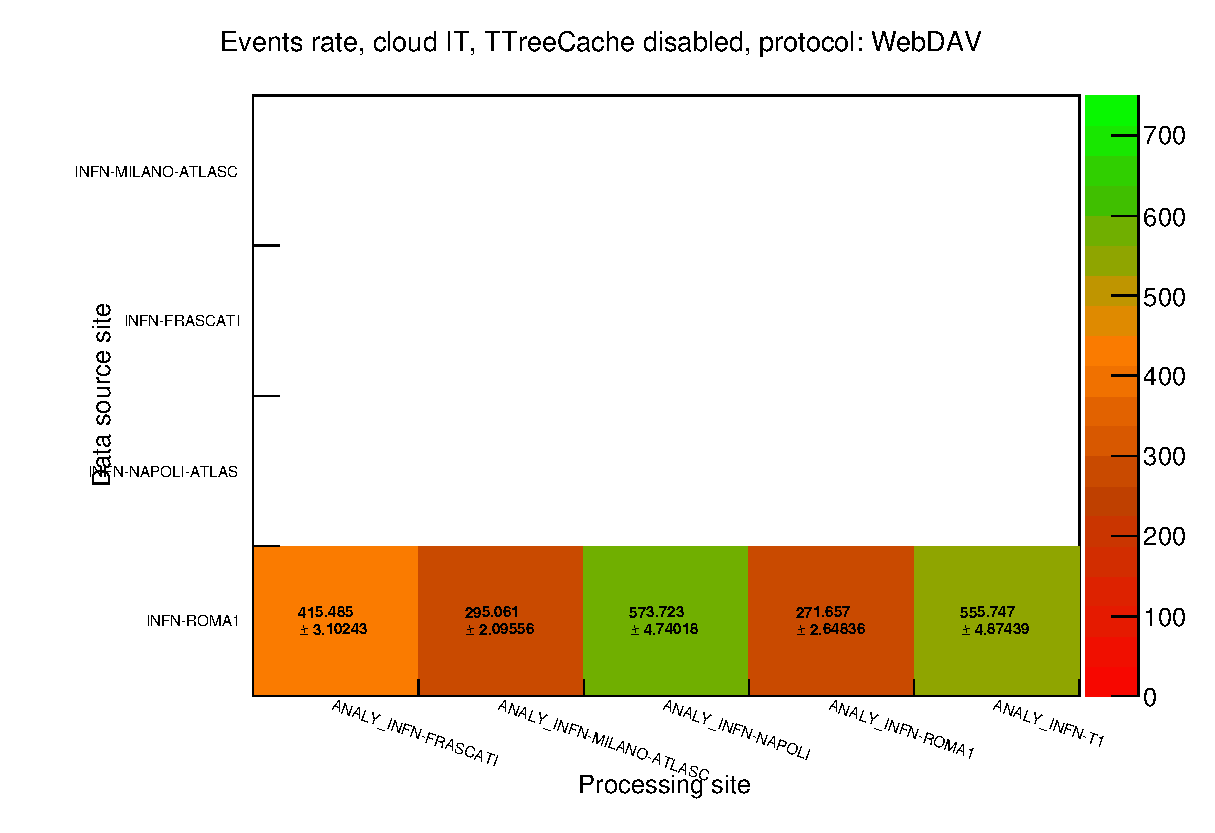
\includegraphics[width=\textwidth]{IT_EventsRate.eps}
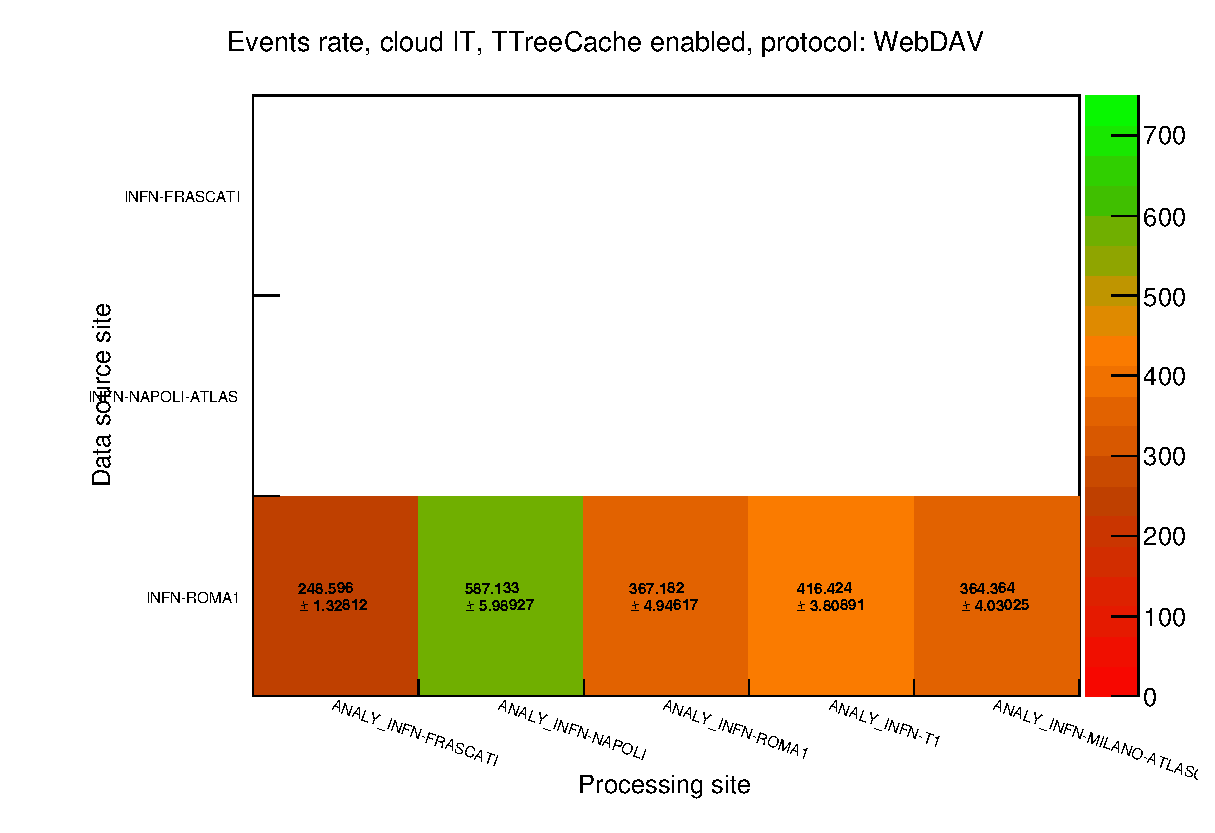
\includegraphics[width=\textwidth]{IT_tEventsRate.eps}
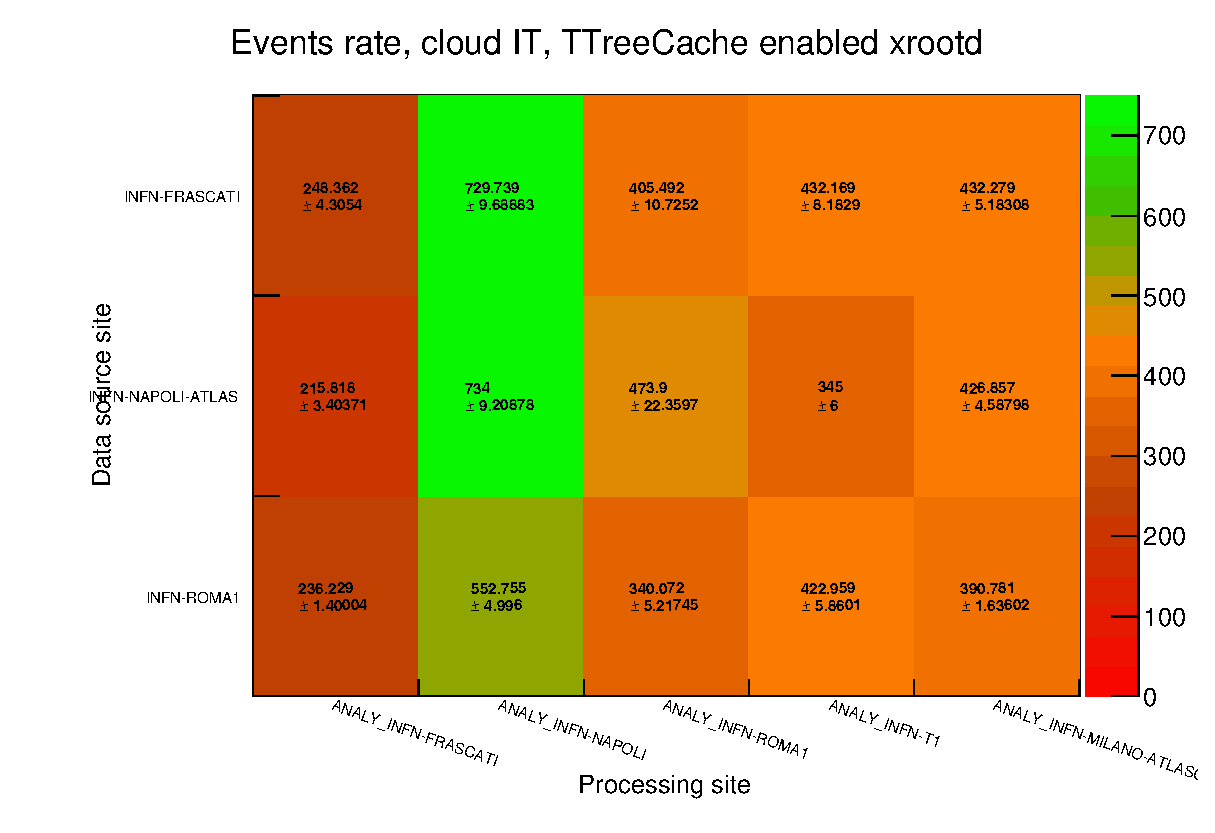
\includegraphics[width=\textwidth]{IT_xEventsRate.eps}
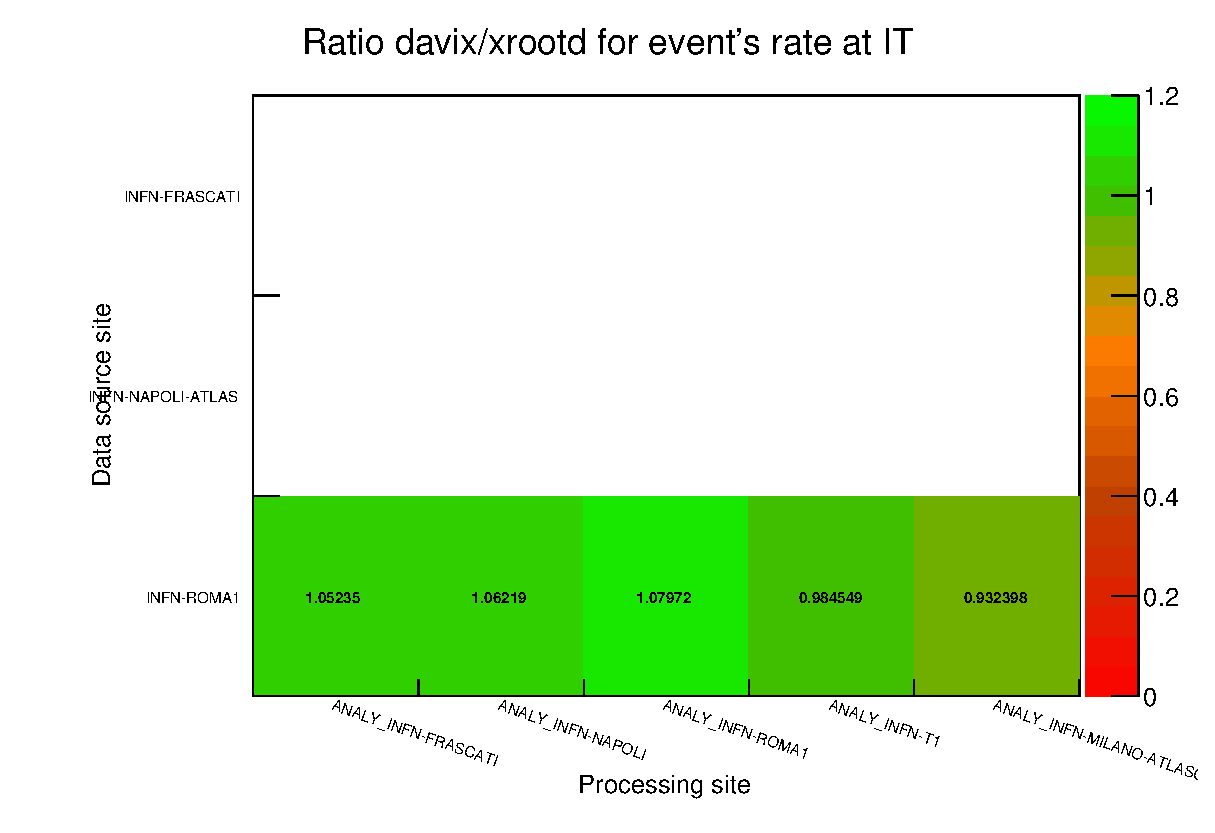
\includegraphics[width=\textwidth]{IT_xRatio.eps}
\vspace{1ex}\\

\subsection{Cloud ND}
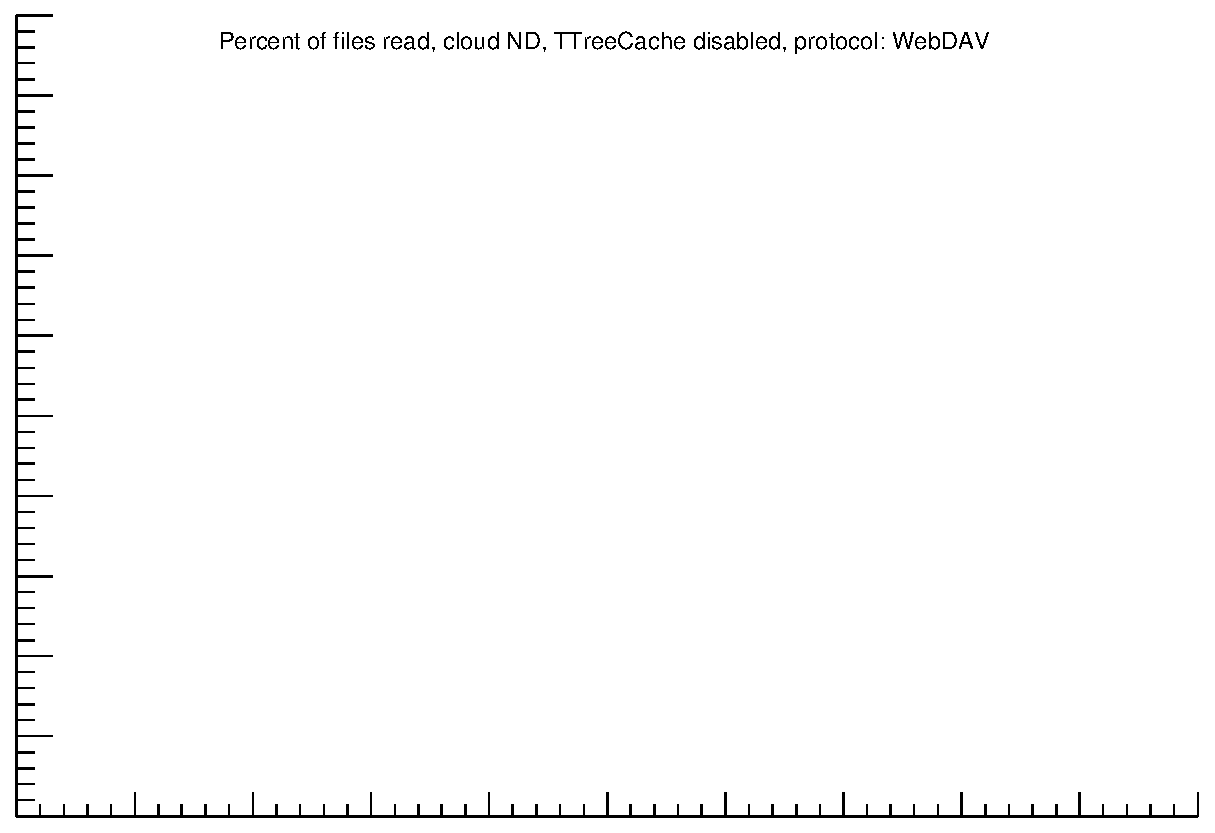
\includegraphics[width=\textwidth]{ND_PerCentFile.eps}
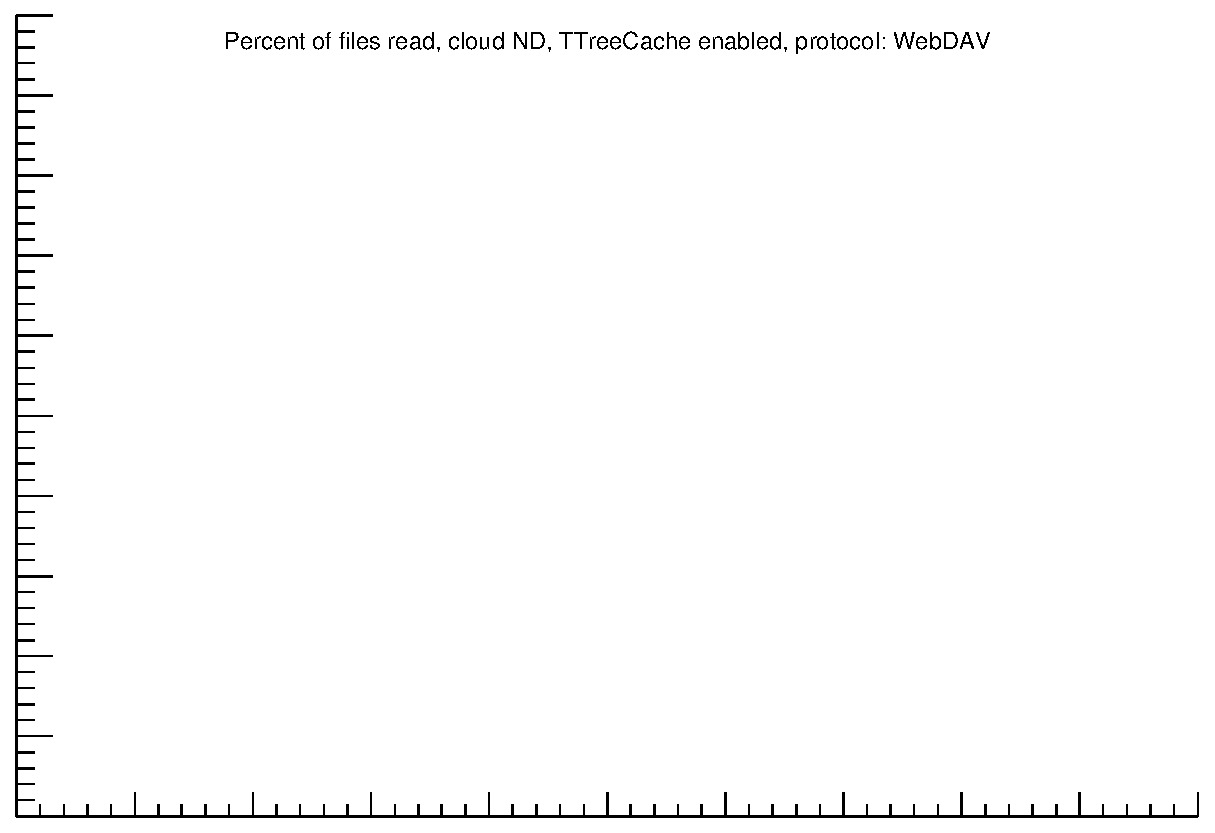
\includegraphics[width=\textwidth]{ND_tPerCentFile.eps}
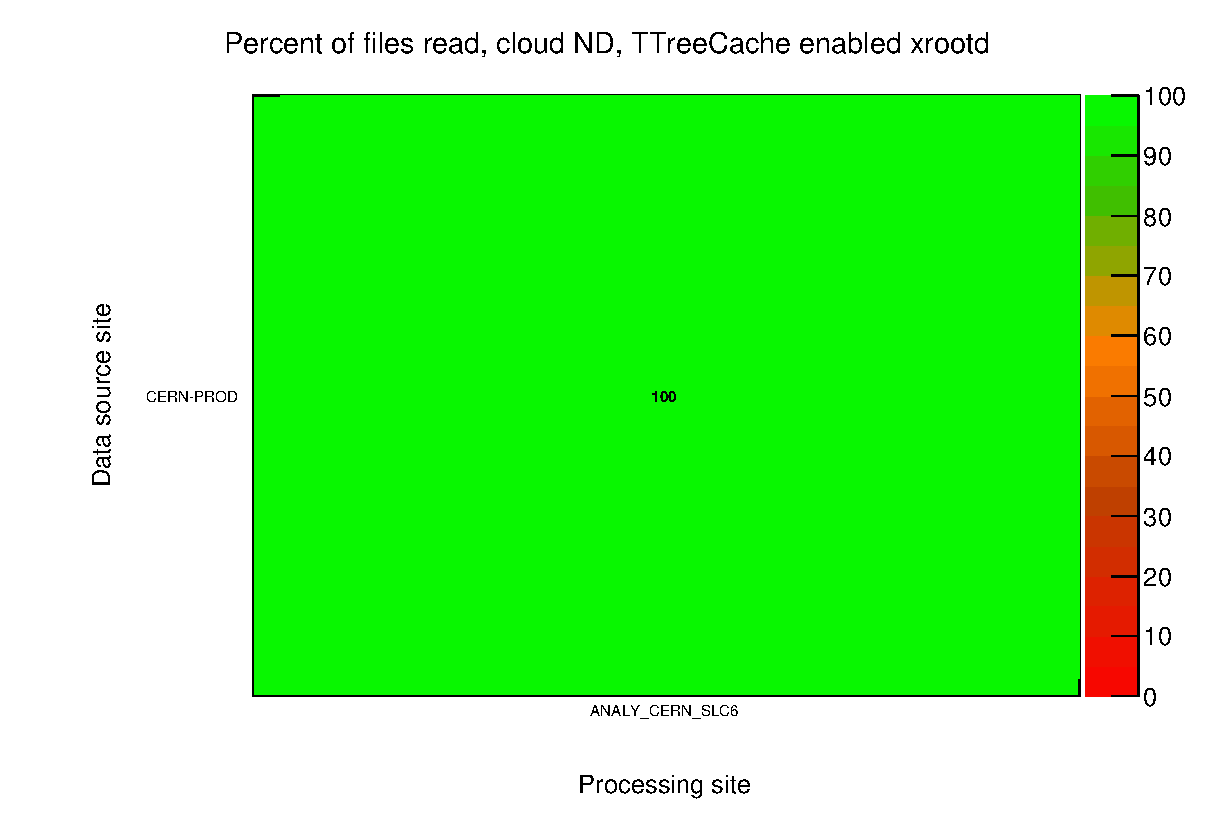
\includegraphics[width=\textwidth]{ND_xPerCentFile.eps}
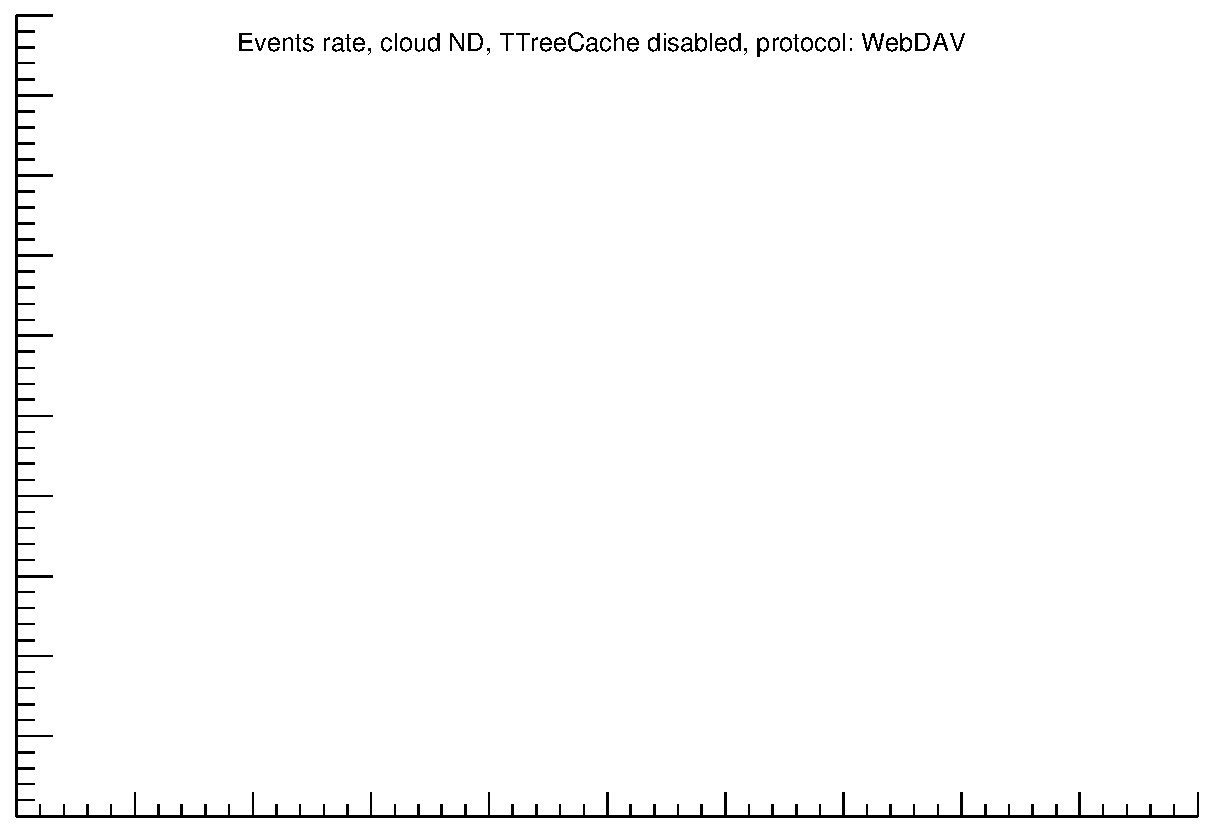
\includegraphics[width=\textwidth]{ND_EventsRate.eps}
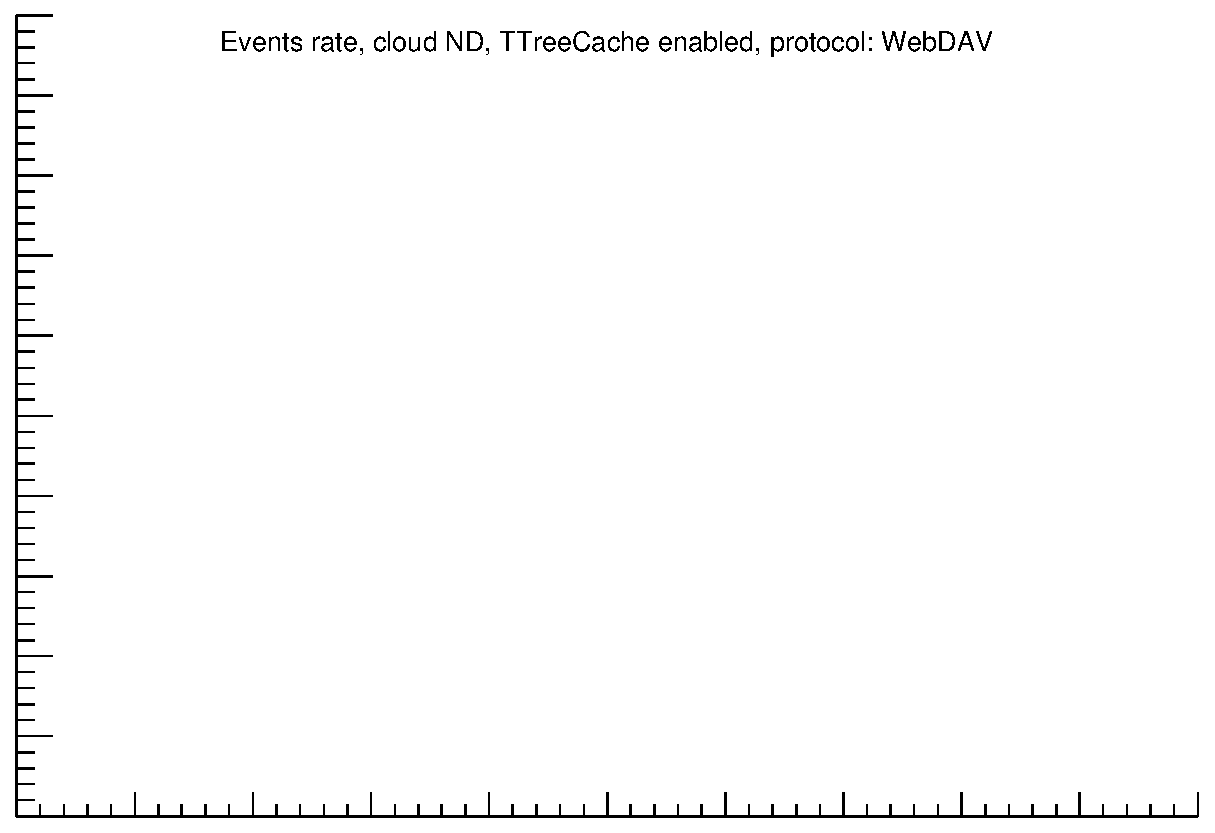
\includegraphics[width=\textwidth]{ND_tEventsRate.eps}
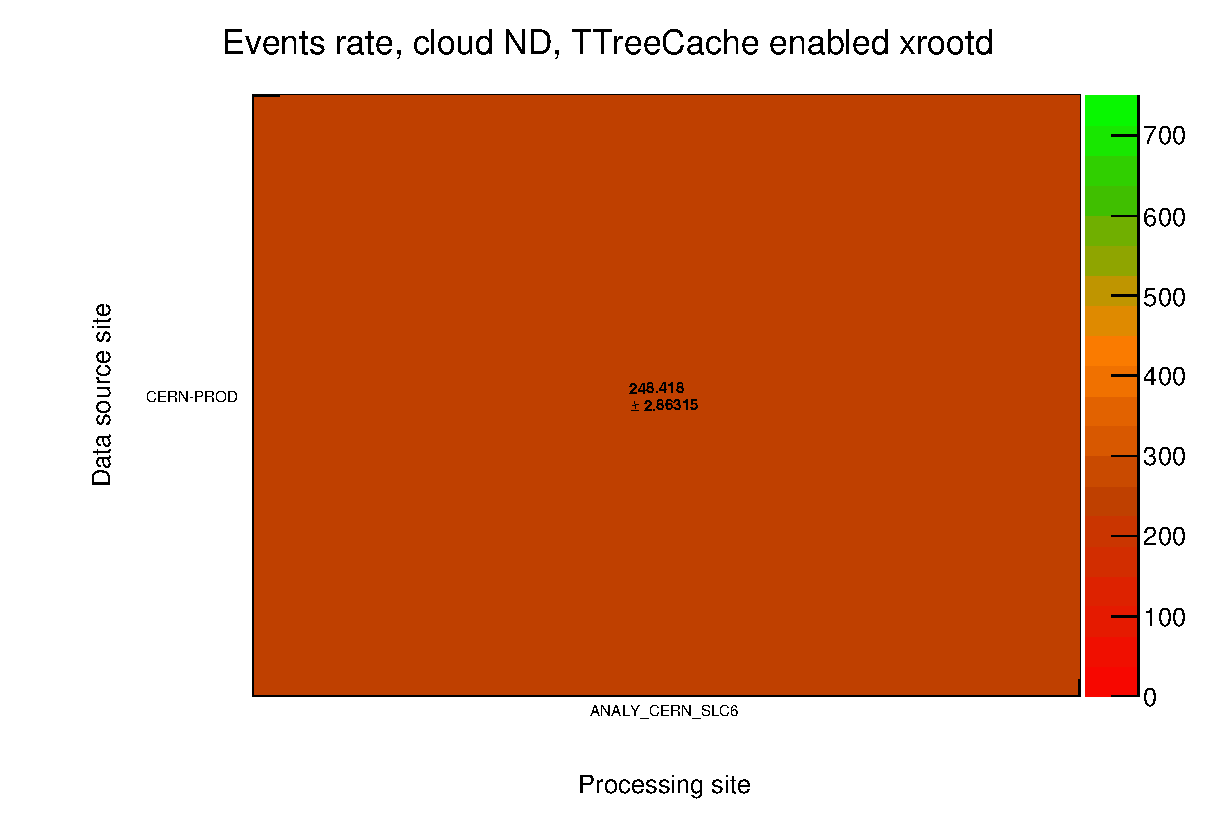
\includegraphics[width=\textwidth]{ND_xEventsRate.eps}
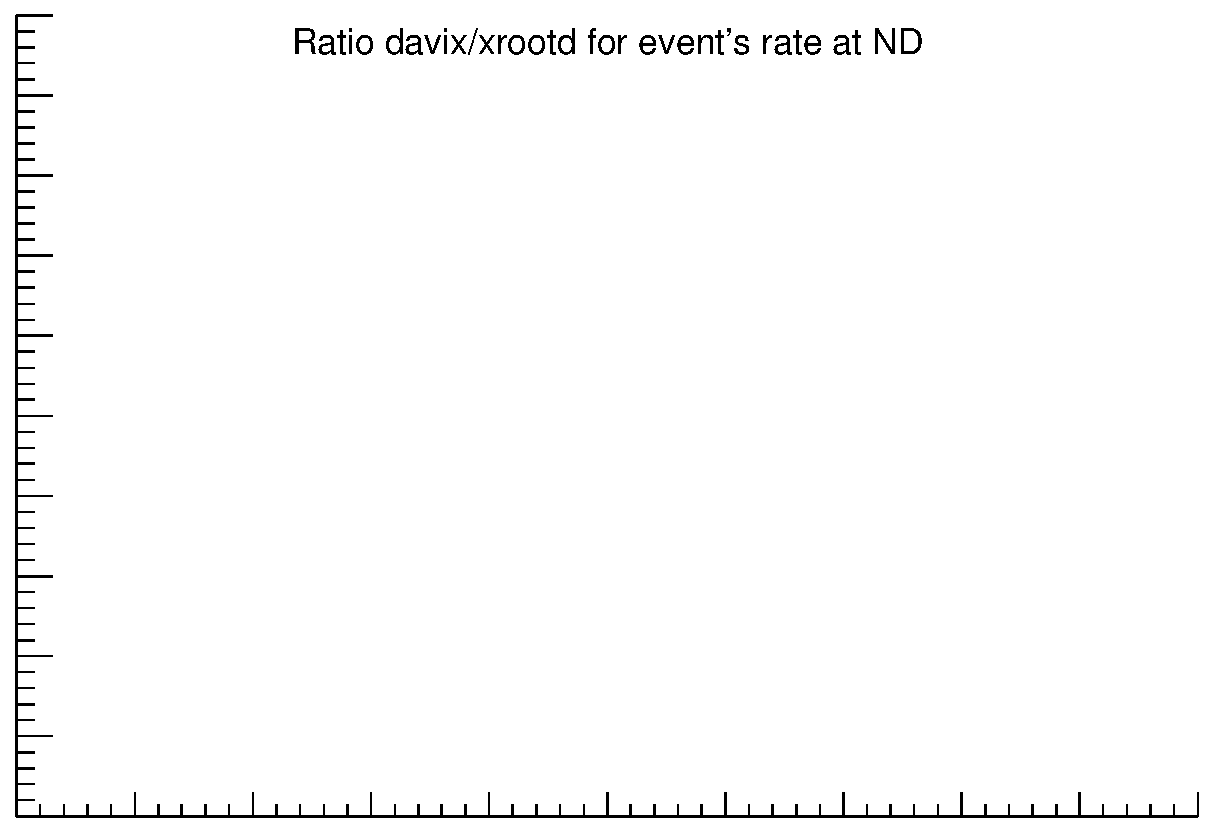
\includegraphics[width=\textwidth]{ND_xRatio.eps}
\vspace{1ex}\\

\subsection{Cloud NL}
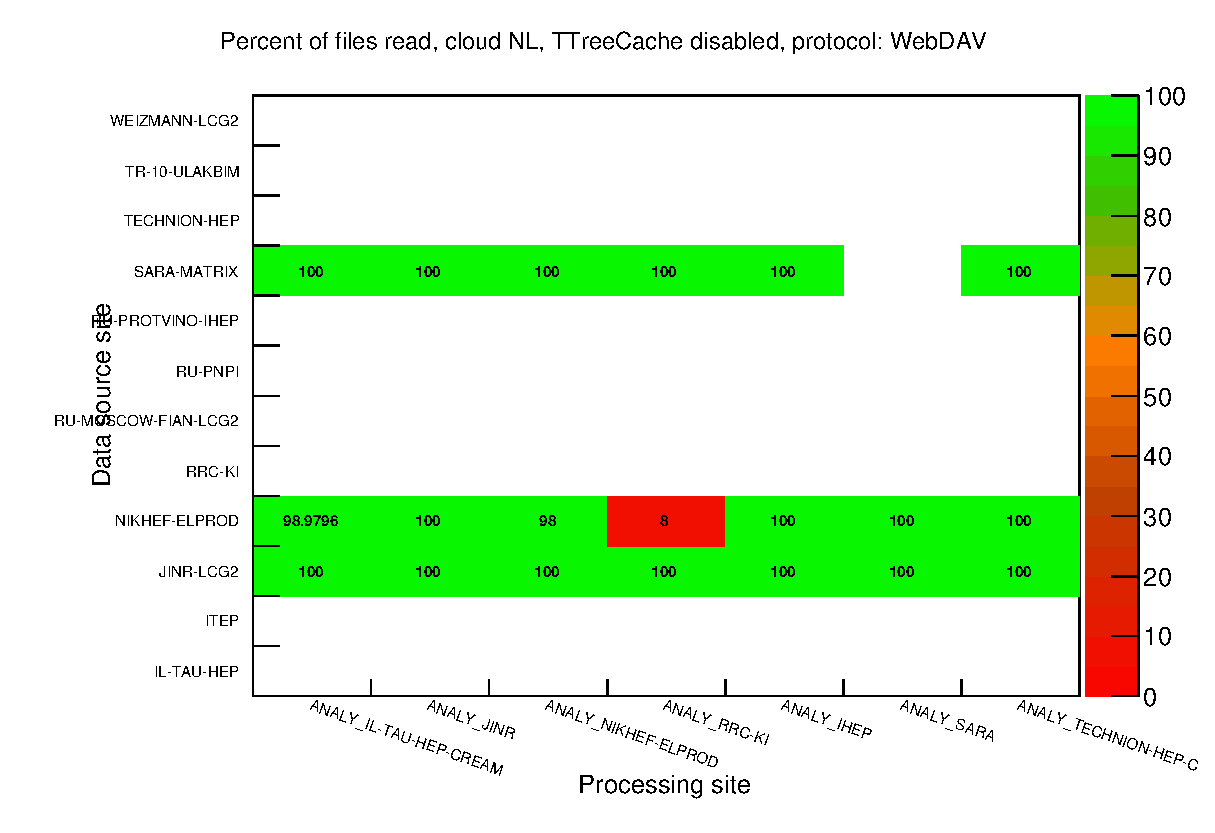
\includegraphics[width=\textwidth]{NL_PerCentFile.eps}
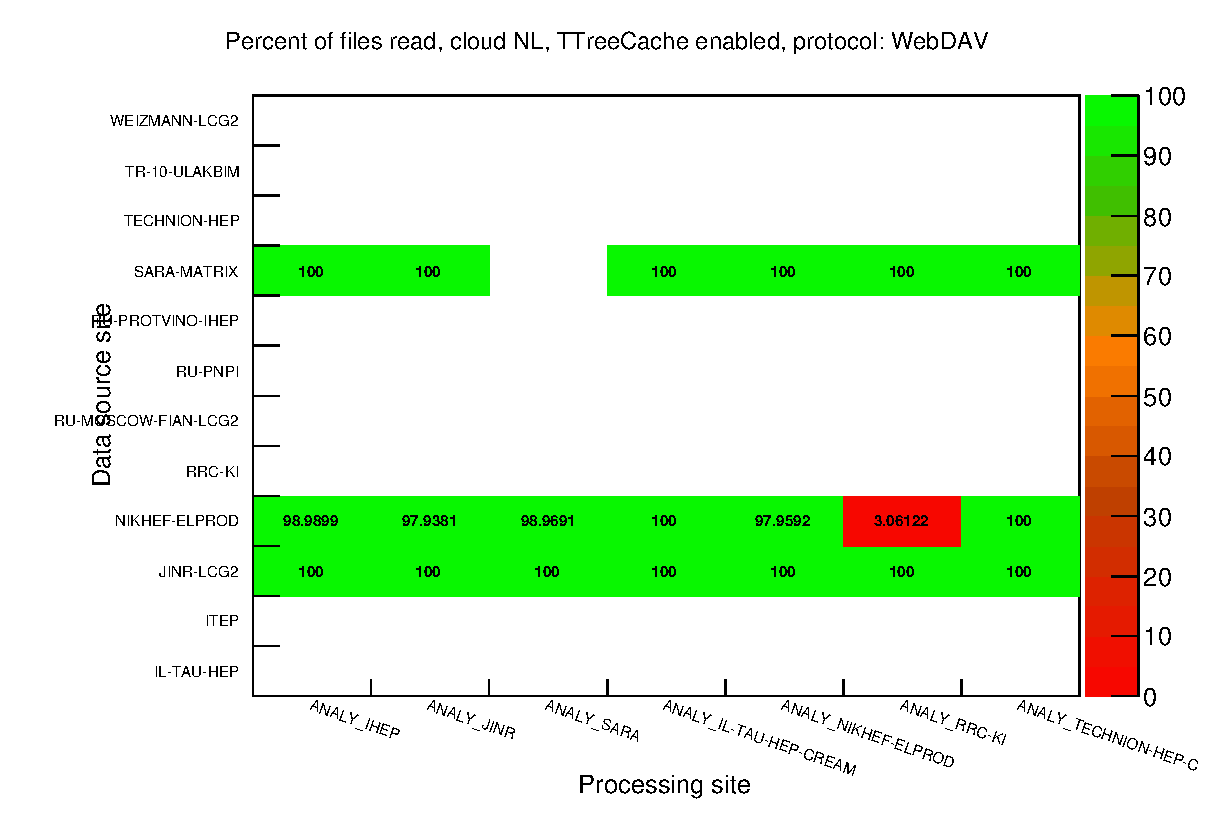
\includegraphics[width=\textwidth]{NL_tPerCentFile.eps}
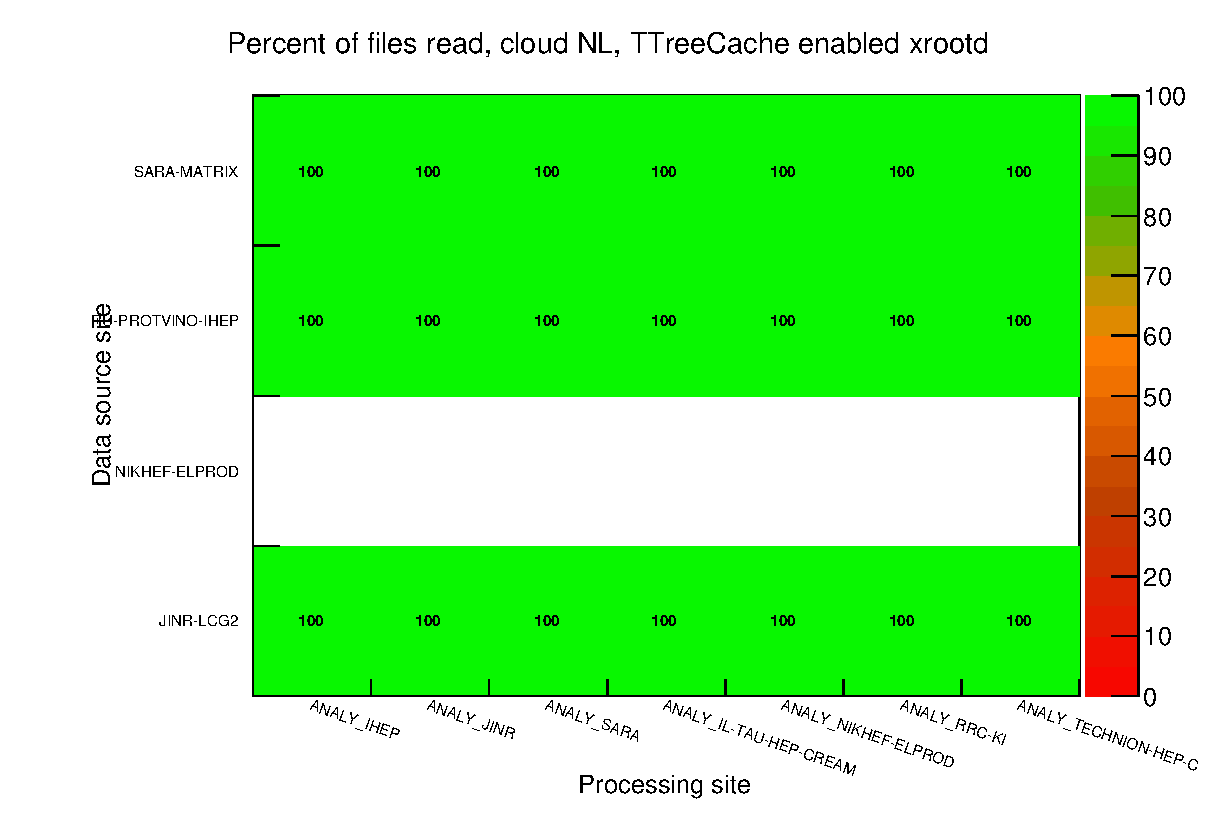
\includegraphics[width=\textwidth]{NL_xPerCentFile.eps}
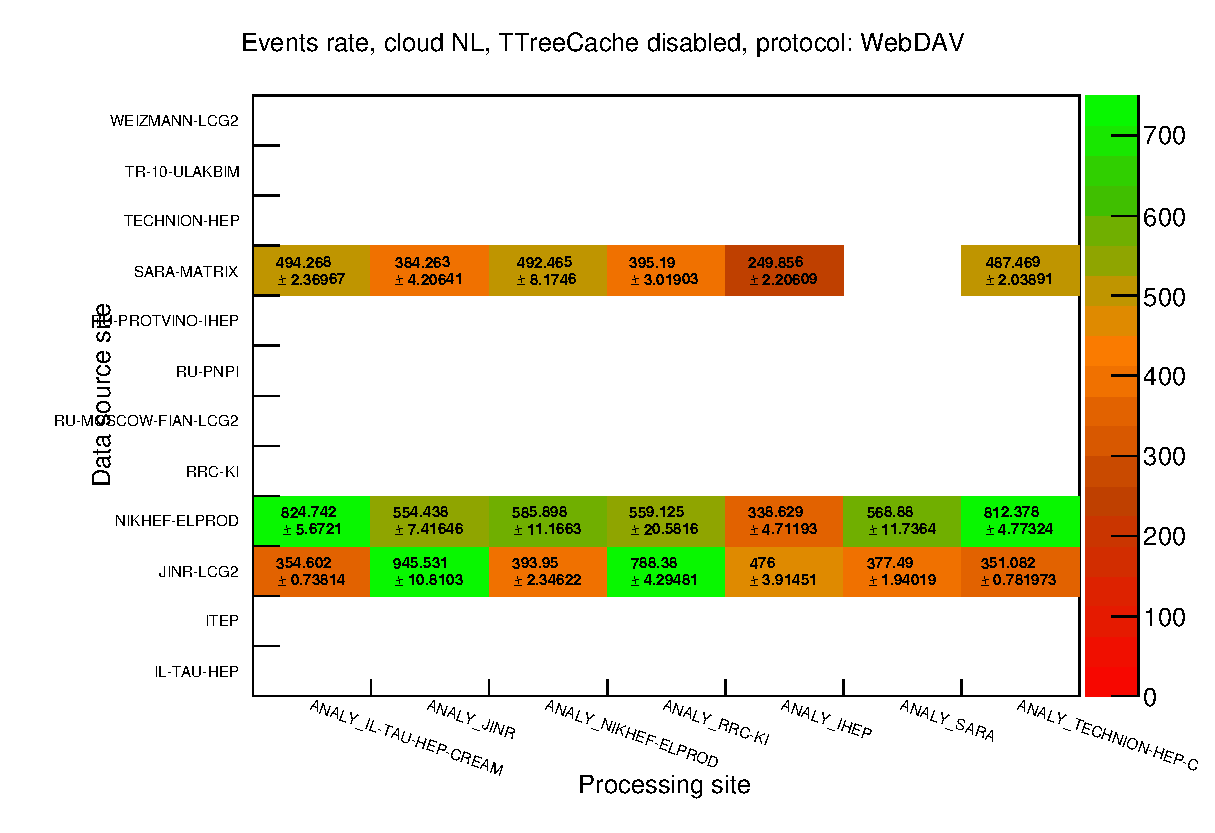
\includegraphics[width=\textwidth]{NL_EventsRate.eps}
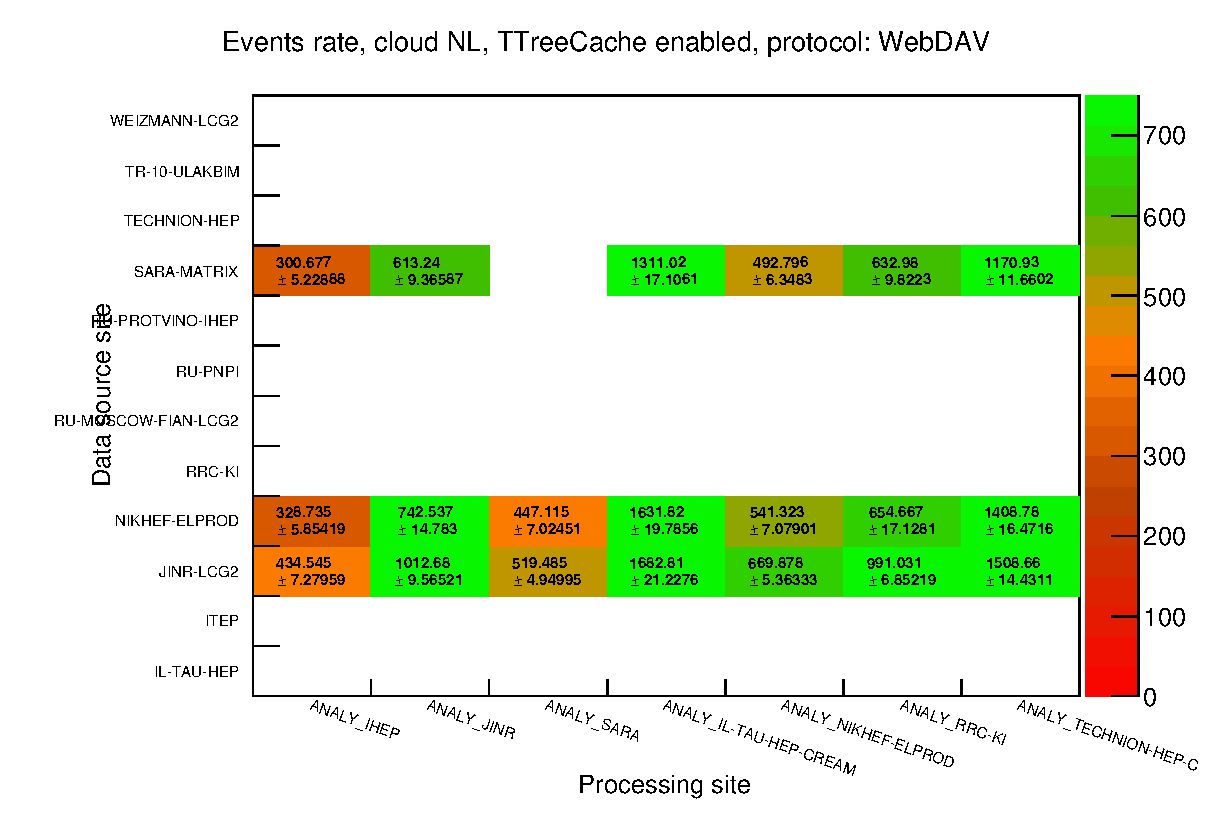
\includegraphics[width=\textwidth]{NL_tEventsRate.eps}
\includegraphics[width=\textwidth]{NL_xEventsRate.eps}
\includegraphics[width=\textwidth]{NL_xRatio.eps}
\vspace{1ex}\\

\subsection{Cloud UK}
\includegraphics[width=\textwidth]{UK_PerCentFile.eps}
\includegraphics[width=\textwidth]{UK_tPerCentFile.eps}
\includegraphics[width=\textwidth]{UK_xPerCentFile.eps}
\includegraphics[width=\textwidth]{UK_EventsRate.eps}
\includegraphics[width=\textwidth]{UK_tEventsRate.eps}
\includegraphics[width=\textwidth]{UK_xEventsRate.eps}
\includegraphics[width=\textwidth]{UK_xRatio.eps}
\vspace{1ex}\\

\subsection{Cloud US}
\includegraphics[width=\textwidth]{US_PerCentFile.eps}
\includegraphics[width=\textwidth]{US_tPerCentFile.eps}
\includegraphics[width=\textwidth]{US_xPerCentFile.eps}
\includegraphics[width=\textwidth]{US_EventsRate.eps}
\includegraphics[width=\textwidth]{US_tEventsRate.eps}
\includegraphics[width=\textwidth]{US_xEventsRate.eps}
\includegraphics[width=\textwidth]{US_xRatio.eps}
\vspace{1ex}\\


\section{The job on the queues}

Jobs with TTreeCache disabled 

\begin{longtable}{|c|c|}

	\hline

	Queue & Job Status\\\hline
	\endhead

	\hline
	\color{black}ANALY\_AUSTRALIA & \color{green}done \\
	\hline
	\color{black}ANALY\_MCGILL & \color{green}done \\
	\hline
	\color{black}ANALY\_SCINET & \color{green}done \\
	\hline
	\color{black}ANALY\_SFU & \color{green}done \\
	\hline
	\color{black}ANALY\_TRIUMF & \color{green}done \\
	\hline
	\color{black}ANALY\_VICTORIA & \color{green}done \\
	\hline
	\color{black}ANALY\_CSCS & \color{red}failed \\
	\hline
	\color{black}ANALY\_CYF & \color{green}done \\
	\hline
	\color{black}ANALY\_DESY-HH & \color{green}done \\
	\hline
	\color{black}ANALY\_DESY-ZN & \color{green}done \\
	\hline
	\color{black}ANALY\_FMPhI-UNIBA & \color{red}failed \\
	\hline
	\color{black}ANALY\_FREIBURG & \color{green}done \\
	\hline
	\color{black}ANALY\_FZK & \color{green}done \\
	\hline
	\color{black}ANALY\_FZU & \color{red}failed \\
	\hline
	\color{black}ANALY\_GOEGRID & \color{green}done \\
	\hline
	\color{black}ANALY\_HEPHY-UIBK & \color{green}done \\
	\hline
	\color{black}ANALY\_IEPSAS-Kosice & \color{green}done \\
	\hline
	\color{black}ANALY\_LRZ & \color{red}failed \\
	\hline
	\color{black}ANALY\_MPPMU & \color{green}done \\
	\hline
	\hline
	\color{black}ANALY\_wuppertalprod & \color{green}done \\
	\hline
	\color{black}ANALY\_PIC\_SL6 & \color{green}done \\
	\hline
	\color{black}ANALY\_UAM & \color{green}done \\
	\hline
	\color{black}ANALY\_UTFSM & \color{green}done \\
	\hline
	\color{black}ANALY\_IFAE & \color{green}done \\
	\hline
	\color{black}ANALY\_IFIC & \color{green}done \\
	\hline
	\color{black}ANALY\_NCG-INGRID-PT\_SL6 & \color{green}done \\
	\hline
	\color{black}ANALY\_BEIJING & \color{green}done \\
	\hline
	\color{black}ANALY\_CPPM & \color{green}done \\
	\hline
	\color{black}ANALY\_GRIF-IRFU & \color{green}done \\
	\hline
	\hline
	\color{black}ANALY\_GRIF-LPNHE & \color{green}done \\
	\hline
	\color{black}ANALY\_IN2P3-CC & \color{red}failed \\
	\hline
	\color{black}ANALY\_LAPP & \color{green}done \\
	\hline
	\color{black}ANALY\_LPC & \color{green}done \\
	\hline
	\color{black}ANALY\_LPSC & \color{green}done \\
	\hline
	\color{black}ANALY\_ROMANIA02 & \color{green}done \\
	\hline
	\color{black}ANALY\_ROMANIA07 & \color{green}done \\
	\hline
	\color{black}ANALY\_TOKYO & \color{red}failed \\
	\hline
	\color{black}ANALY\_INFN-FRASCATI & \color{green}done \\
	\hline
	\color{black}ANALY\_INFN-MILANO-ATLASC & \color{green}done \\
	\hline
	\color{black}ANALY\_INFN-NAPOLI & \color{green}done \\
	\hline
	\color{black}ANALY\_INFN-ROMA1 & \color{green}done \\
	\hline
	\color{black}ANALY\_INFN-T1 & \color{green}done \\
	\hline
	\hline
	\color{black}ANALY\_LUNARC & \color{green}done \\
	\hline
	\color{black}ANALY\_UNIBE-LHEP & \color{red}failed \\
	\hline
	\color{black}ANALY\_CERN\_CLOUD & \color{red}failed \\
	\hline
	\color{black}ANALY\_CERN\_SLC6 & \color{green}done \\
	\hline
	\color{black}ANALY\_IL-TAU-HEP-CREAM & \color{green}done \\
	\hline
	\color{black}ANALY\_JINR & \color{green}done \\
	\hline
	\color{black}ANALY\_NIKHEF-ELPROD & \color{green}done \\
	\hline
	\color{black}ANALY\_RRC-KI & \color{green}done \\
	\hline
	\color{black}ANALY\_IHEP & \color{green}done \\
	\hline
	\color{black}ANALY\_SARA & \color{green}done \\
	\hline
	\color{black}ANALY\_TECHNION-HEP-CREAM & \color{green}done \\
	\hline
	\color{black}ANALY\_TR-10-ULAKBIM & \color{red}failed \\
	\hline
	\color{black}ANALY\_WEIZMANN-CREAM & \color{green}done \\
	\hline
	\color{black}ANALY\_RALPP\_SL6 & \color{green}done \\
	\hline
	\color{black}ANALY\_RAL\_SL6 & \color{green}done \\
	\hline
	\color{black}ANALY\_BHAM\_SL6 & \color{green}done \\
	\hline
	\color{black}ANALY\_CAM\_SL6 & \color{green}done \\
	\hline
	\color{black}ANALY\_ECDF\_SL6 & \color{green}done \\
	\hline
	\color{black}ANALY\_GLASGOW\_SL6 & \color{green}done \\
	\hline
	\color{black}ANALY\_LANCS\_SL6 & \color{green}done \\
	\hline
	\color{black}ANALY\_LIV\_SL6 & \color{green}done \\
	\hline
	\color{black}ANALY\_MANC\_SL6 & \color{green}done \\
	\hline
	\color{black}ANALY\_OX\_SL6 & \color{green}done \\
	\hline
	\color{black}ANALY\_QMUL\_SL6 & \color{green}done \\
	\hline
	\color{black}ANALY\_RHUL\_SL6 & \color{green}done \\
	\hline
	\color{black}ANALY\_SHEF\_SL6 & \color{green}done \\
	\hline
	\color{black}ANALY\_UCL\_SL6 & \color{green}done \\
	\hline
	\color{black}ANALY\_AGLT2\_SL6 & \color{green}done \\
	\hline
	\color{black}ANALY\_BNL\_CLOUD & \color{green}done \\
	\hline
	\color{black}ANALY\_BU\_ATLAS\_Tier2\_SL6 & \color{green}done \\
	\hline
	\color{black}ANALY\_MWT2\_SL6 & \color{green}done \\
	\hline
	\color{black}ANALY\_OU\_OCHEP\_SWT2 & \color{red}failed \\
	\hline
	\color{black}ANALY\_SLAC & \color{green}done \\
	\hline
	\color{black}ANALY\_SWT2\_CPB & \color{green}done \\
	\hline
	\color{black}ANALY\_TAIWAN\_SL6 & \color{green}done \\
\hline

\end{longtable}
\includegraphics[width=\textwidth]{../PieChart/job/mcanvas.eps}
Jobs with TTreeCache enabled 

\begin{longtable}{|c|c|}

	\hline

	Queue & Job Status\\\hline
	\endhead

	\hline
	\color{black}ANALY\_AUSTRALIA & \color{green}done \\
	\hline
	\color{black}ANALY\_MCGILL & \color{green}done \\
	\hline
	\color{black}ANALY\_SCINET & \color{green}done \\
	\hline
	\color{black}ANALY\_SFU & \color{green}done \\
	\hline
	\color{black}ANALY\_TRIUMF & \color{green}done \\
	\hline
	\color{black}ANALY\_VICTORIA & \color{green}done \\
	\hline
	\color{black}ANALY\_CSCS & \color{red}failed \\
	\hline
	\color{black}ANALY\_CYF & \color{green}done \\
	\hline
	\color{black}ANALY\_DESY-HH & \color{green}done \\
	\hline
	\color{black}ANALY\_DESY-ZN & \color{green}done \\
	\hline
	\color{black}ANALY\_FMPhI-UNIBA & \color{red}failed \\
	\hline
	\color{black}ANALY\_FREIBURG & \color{green}done \\
	\hline
	\color{black}ANALY\_FZK & \color{green}done \\
	\hline
	\color{black}ANALY\_FZU & \color{red}failed \\
	\hline
	\color{black}ANALY\_GOEGRID & \color{green}done \\
	\hline
	\color{black}ANALY\_HEPHY-UIBK & \color{green}done \\
	\hline
	\color{black}ANALY\_IEPSAS-Kosice & \color{green}done \\
	\hline
	\color{black}ANALY\_LRZ & \color{red}failed \\
	\hline
	\color{black}ANALY\_MPPMU & \color{green}done \\
	\hline
	\hline
	\color{black}ANALY\_wuppertalprod & \color{green}done \\
	\hline
	\color{black}ANALY\_PIC\_SL6 & \color{green}done \\
	\hline
	\color{black}ANALY\_UAM & \color{green}done \\
	\hline
	\color{black}ANALY\_UTFSM & \color{green}done \\
	\hline
	\color{black}ANALY\_IFAE & \color{green}done \\
	\hline
	\color{black}ANALY\_IFIC & \color{green}done \\
	\hline
	\color{black}ANALY\_NCG-INGRID-PT\_SL6 & \color{green}done \\
	\hline
	\color{black}ANALY\_BEIJING & \color{green}done \\
	\hline
	\color{black}ANALY\_CPPM & \color{red}failed \\
	\hline
	\color{black}ANALY\_GRIF-IRFU & \color{green}done \\
	\hline
	\hline
	\color{black}ANALY\_GRIF-LPNHE & \color{green}done \\
	\hline
	\color{black}ANALY\_IN2P3-CC & \color{green}done \\
	\hline
	\color{black}ANALY\_LAPP & \color{green}done \\
	\hline
	\color{black}ANALY\_LPC & \color{green}done \\
	\hline
	\color{black}ANALY\_LPSC & \color{green}done \\
	\hline
	\color{black}ANALY\_ROMANIA02 & \color{green}done \\
	\hline
	\color{black}ANALY\_ROMANIA07 & \color{green}done \\
	\hline
	\color{black}ANALY\_TOKYO & \color{green}done \\
	\hline
	\color{black}ANALY\_INFN-FRASCATI & \color{green}done \\
	\hline
	\color{black}ANALY\_INFN-MILANO-ATLASC & \color{green}done \\
	\hline
	\color{black}ANALY\_INFN-NAPOLI & \color{green}done \\
	\hline
	\color{black}ANALY\_INFN-ROMA1 & \color{green}done \\
	\hline
	\color{black}ANALY\_INFN-T1 & \color{green}done \\
	\hline
	\hline
	\color{black}ANALY\_LUNARC & \color{green}done \\
	\hline
	\color{black}ANALY\_UNIBE-LHEP & \color{red}failed \\
	\hline
	\color{black}ANALY\_CERN\_CLOUD & \color{red}failed \\
	\hline
	\color{black}ANALY\_CERN\_SLC6 & \color{green}done \\
	\hline
	\color{black}ANALY\_IL-TAU-HEP-CREAM & \color{green}done \\
	\hline
	\color{black}ANALY\_JINR & \color{green}done \\
	\hline
	\color{black}ANALY\_NIKHEF-ELPROD & \color{green}done \\
	\hline
	\color{black}ANALY\_RRC-KI & \color{green}done \\
	\hline
	\color{black}ANALY\_IHEP & \color{green}done \\
	\hline
	\color{black}ANALY\_SARA & \color{green}done \\
	\hline
	\color{black}ANALY\_TECHNION-HEP-CREAM & \color{green}done \\
	\hline
	\color{black}ANALY\_TR-10-ULAKBIM & \color{red}failed \\
	\hline
	\color{black}ANALY\_WEIZMANN-CREAM & \color{green}done \\
	\hline
	\color{black}ANALY\_RALPP\_SL6 & \color{red}failed \\
	\hline
	\color{black}ANALY\_RAL\_SL6 & \color{red}failed \\
	\hline
	\color{black}ANALY\_BHAM\_SL6 & \color{red}failed \\
	\hline
	\color{black}ANALY\_CAM\_SL6 & \color{red}failed \\
	\hline
	\color{black}ANALY\_ECDF\_SL6 & \color{red}failed \\
	\hline
	\color{black}ANALY\_GLASGOW\_SL6 & \color{red}failed \\
	\hline
	\color{black}ANALY\_LANCS\_SL6 & \color{red}failed \\
	\hline
	\color{black}ANALY\_LIV\_SL6 & \color{red}failed \\
	\hline
	\color{black}ANALY\_MANC\_SL6 & \color{red}failed \\
	\hline
	\color{black}ANALY\_OX\_SL6 & \color{red}failed \\
	\hline
	\color{black}ANALY\_QMUL\_SL6 & \color{red}failed \\
	\hline
	\color{black}ANALY\_RHUL\_SL6 & \color{red}failed \\
	\hline
	\color{black}ANALY\_SHEF\_SL6 & \color{red}failed \\
	\hline
	\color{black}ANALY\_UCL\_SL6 & \color{green}done \\
	\hline
	\color{black}ANALY\_AGLT2\_SL6 & \color{green}done \\
	\hline
	\color{black}ANALY\_BNL\_CLOUD & \color{green}done \\
	\hline
	\color{black}ANALY\_BU\_ATLAS\_Tier2\_SL6 & \color{red}failed \\
	\hline
	\color{black}ANALY\_MWT2\_SL6 & \color{green}done \\
	\hline
	\color{black}ANALY\_OU\_OCHEP\_SWT2 & \color{red}failed \\
	\hline
	\color{black}ANALY\_SLAC & \color{green}done \\
	\hline
	\color{black}ANALY\_SWT2\_CPB & \color{red}failed \\
	\hline
	\color{black}ANALY\_TAIWAN\_SL6 & \color{green}done \\
\hline

\end{longtable}
\includegraphics[width=\textwidth]{../PieChart/job/tcanvas.eps}
Jobs with xrootd (TTreeCache enabled) 

\begin{longtable}{|c|c|}

	\hline

	Queue & Job Status\\\hline
	\endhead

	\hline
	\color{black}ANALY\_AUSTRALIA & \color{green}done \\
	\hline
	\color{black}ANALY\_MCGILL & \color{green}done \\
	\hline
	\color{black}ANALY\_SCINET & \color{green}done \\
	\hline
	\color{black}ANALY\_SFU & \color{green}done \\
	\hline
	\color{black}ANALY\_TRIUMF & \color{green}done \\
	\hline
	\color{black}ANALY\_VICTORIA & \color{green}done \\
	\hline
	\color{black}ANALY\_CSCS & \color{red}failed \\
	\hline
	\color{black}ANALY\_CYF & \color{green}done \\
	\hline
	\color{black}ANALY\_DESY-HH & \color{green}done \\
	\hline
	\color{black}ANALY\_DESY-ZN & \color{green}done \\
	\hline
	\color{black}ANALY\_FMPhI-UNIBA & \color{red}failed \\
	\hline
	\color{black}ANALY\_FREIBURG & \color{green}done \\
	\hline
	\color{black}ANALY\_FZK & \color{green}done \\
	\hline
	\color{black}ANALY\_FZU & \color{green}done \\
	\hline
	\color{black}ANALY\_GOEGRID & \color{green}done \\
	\hline
	\color{black}ANALY\_HEPHY-UIBK & \color{green}done \\
	\hline
	\color{black}ANALY\_IEPSAS-Kosice & \color{green}done \\
	\hline
	\color{black}ANALY\_LRZ & \color{red}failed \\
	\hline
	\color{black}ANALY\_MPPMU & \color{green}done \\
	\hline
	\hline
	\color{black}ANALY\_wuppertalprod & \color{green}done \\
	\hline
	\color{black}ANALY\_PIC\_SL6 & \color{green}done \\
	\hline
	\color{black}ANALY\_UAM & \color{green}done \\
	\hline
	\color{black}ANALY\_UTFSM & \color{green}done \\
	\hline
	\color{black}ANALY\_IFAE & \color{green}done \\
	\hline
	\color{black}ANALY\_IFIC & \color{green}done \\
	\hline
	\color{black}ANALY\_NCG-INGRID-PT\_SL6 & \color{green}done \\
	\hline
	\color{black}ANALY\_BEIJING & \color{green}done \\
	\hline
	\color{black}ANALY\_CPPM & \color{green}done \\
	\hline
	\color{black}ANALY\_GRIF-IRFU & \color{green}done \\
	\hline
	\hline
	\color{black}ANALY\_GRIF-LPNHE & \color{green}done \\
	\hline
	\color{black}ANALY\_IN2P3-CC & \color{green}done \\
	\hline
	\color{black}ANALY\_LAPP & \color{green}done \\
	\hline
	\color{black}ANALY\_LPC & \color{green}done \\
	\hline
	\color{black}ANALY\_LPSC & \color{green}done \\
	\hline
	\color{black}ANALY\_ROMANIA02 & \color{green}done \\
	\hline
	\color{black}ANALY\_ROMANIA07 & \color{green}done \\
	\hline
	\color{black}ANALY\_TOKYO & \color{green}done \\
	\hline
	\color{black}ANALY\_INFN-FRASCATI & \color{green}done \\
	\hline
	\color{black}ANALY\_INFN-MILANO-ATLASC & \color{green}done \\
	\hline
	\color{black}ANALY\_INFN-NAPOLI & \color{green}done \\
	\hline
	\color{black}ANALY\_INFN-ROMA1 & \color{green}done \\
	\hline
	\color{black}ANALY\_INFN-T1 & \color{green}done \\
	\hline
	\hline
	\color{black}ANALY\_LUNARC & \color{green}done \\
	\hline
	\color{black}ANALY\_UNIBE-LHEP & \color{red}failed \\
	\hline
	\color{black}ANALY\_CERN\_CLOUD & \color{red}failed \\
	\hline
	\color{black}ANALY\_CERN\_SLC6 & \color{green}done \\
	\hline
	\color{black}ANALY\_IL-TAU-HEP-CREAM & \color{green}done \\
	\hline
	\color{black}ANALY\_JINR & \color{green}done \\
	\hline
	\color{black}ANALY\_NIKHEF-ELPROD & \color{green}done \\
	\hline
	\color{black}ANALY\_RRC-KI & \color{green}done \\
	\hline
	\color{black}ANALY\_IHEP & \color{green}done \\
	\hline
	\color{black}ANALY\_SARA & \color{green}done \\
	\hline
	\color{black}ANALY\_TECHNION-HEP-CREAM & \color{green}done \\
	\hline
	\color{black}ANALY\_TR-10-ULAKBIM & \color{red}failed \\
	\hline
	\color{black}ANALY\_WEIZMANN-CREAM & \color{green}done \\
	\hline
	\color{black}ANALY\_RALPP\_SL6 & \color{green}done \\
	\hline
	\color{black}ANALY\_RAL\_SL6 & \color{green}done \\
	\hline
	\color{black}ANALY\_BHAM\_SL6 & \color{green}done \\
	\hline
	\color{black}ANALY\_CAM\_SL6 & \color{green}done \\
	\hline
	\color{black}ANALY\_ECDF\_SL6 & \color{green}done \\
	\hline
	\color{black}ANALY\_GLASGOW\_SL6 & \color{green}done \\
	\hline
	\color{black}ANALY\_LANCS\_SL6 & \color{green}done \\
	\hline
	\color{black}ANALY\_LIV\_SL6 & \color{green}done \\
	\hline
	\color{black}ANALY\_MANC\_SL6 & \color{green}done \\
	\hline
	\color{black}ANALY\_OX\_SL6 & \color{green}done \\
	\hline
	\color{black}ANALY\_QMUL\_SL6 & \color{green}done \\
	\hline
	\color{black}ANALY\_RHUL\_SL6 & \color{green}done \\
	\hline
	\color{black}ANALY\_SHEF\_SL6 & \color{green}done \\
	\hline
	\color{black}ANALY\_UCL\_SL6 & \color{green}done \\
	\hline
	\color{black}ANALY\_AGLT2\_SL6 & \color{green}done \\
	\hline
	\color{black}ANALY\_BNL\_CLOUD & \color{green}done \\
	\hline
	\color{black}ANALY\_BU\_ATLAS\_Tier2\_SL6 & \color{green}done \\
	\hline
	\color{black}ANALY\_MWT2\_SL6 & \color{green}done \\
	\hline
	\color{black}ANALY\_OU\_OCHEP\_SWT2 & \color{red}failed \\
	\hline
	\color{black}ANALY\_SLAC & \color{green}done \\
	\hline
	\color{black}ANALY\_SWT2\_CPB & \color{green}done \\
	\hline
	\color{black}ANALY\_TAIWAN\_SL6 & \color{green}done \\
\hline

\end{longtable}
\includegraphics[width=\textwidth]{../PieChart/job/xcanvas.eps}






\end{document}

%

% ****** End of file report.tex ******
